% 
% Modelo para Trabalhos Acadêmicos (tese de doutorado, dissertação de mestrado) utilizando a classe abntex2
%
% Modificações: 07/02/2024: Wagner O. Araujo, adequação do template para a IFG - Campus: Anápolis
% ------------------------------------------------------------------------
% ------------------------------------------------------------------------

\documentclass[
	% -- opções da classe memoir --
	12pt,				% tamanho da fonte
	%openright,			% capítulos começam em pág ímpar (insere página vazia caso preciso)
	oneside,			% para impressão no anverso. Oposto a twoside
	a4paper,			% tamanho do papel. 
	% -- opções da classe abntex2 --
	chapter=TITLE,		% títulos de capítulos convertidos em letras maiúsculas
	%section=TITLE,		% títulos de seções convertidos em letras maiúsculas
	%subsection=TITLE,	% títulos de subseções convertidos em letras maiúsculas
	%subsubsection=TITLE,% títulos de subsubseções convertidos em letras maiúsculas
	% -- opções do pacote babel --
	english,			% idioma adicional para hifenização
	%french,			% idioma adicional para hifenização
	%spanish,			% idioma adicional para hifenização
	brazil				% o último idioma é o principal do documento
	]{abntex2}
\usepackage{tabularx}
\usepackage{array}
\usepackage{setup/ufscthesisA4-alf}
\usepackage{multirow}
\usepackage{enumitem}  % Para [label=\alph*)]
\usepackage[table,xcdraw]{xcolor}
\usepackage[htt]{hyphenat} %A opção [htt] avisa ao LaTeX que todos os comandos \texttt do documento passam a aceitar hifenização automática.
%\usepackage[utf8]{inputenc}
%\usepackage[latin1]{inputenc}
%\usepackage[T1]{fontenc}
%\usepackage{lmodern}
\usepackage{microtype}
\usepackage[brazil]{babel}
%\usepackage[portuguese]{babel}
\usepackage{float}
\usepackage{caption}
\usepackage{threeparttable} % Adicione ao preâmbulo
\usepackage{longtable}%para tabelas que ultrapassam uma pagina
\usepackage{booktabs}
\usepackage{siunitx}   % Para o comando \num e formatação de números
\usepackage{blindtext}
%-----------------------------------
\usepackage{readarray} % Pacote para lidar com matrizes
%-----------------------------------
\usepackage{siunitx}
\usepackage{amssymb}
%\usepackage{subfigure}
\usepackage{subcaption}
\usepackage{amsmath}
\usepackage{setspace}
%\usepackage{geometry}
\usepackage{verbatim}
\usepackage{fancyvrb}
\RequirePackage[vlined,titlenumbered,algo2e,ruled,portugues]{setup/algorithm2e}
%--------------------------------------------
\usepackage{fvextra}   % adiciona breaklines, breakanywhere etc. - para o codigo no apendice
%--------------------------------------------
%\usepackage{algorithm}

\usepackage{float}%para colocar a figura na pagina

\usepackage{algpseudocode}
%--------------------------
%---Pacotes graficos
\usepackage{pgfplots}

%\usetikzlibrary{patterns}
\usetikzlibrary{calc}
%\usepackage{graphicx}
\usepackage{tgheros}
\usepackage{xcolor}
\usepackage{url}%foi utilizado para apresentar a url colorida no texto
%----------------------------
%pacote para desenho
\usepackage{pstricks}
\usepackage{tikz}
\usetikzlibrary{shapes.geometric, arrows.meta, positioning, calc}
\usepackage{pgfplots}%pacote para graficos
\usepackage{pgfplotstable}
\pgfplotsset{compat=1.18}
\usepackage{times}%utilizando fonte times new roman
%\usepackage{filecontents}% ativando um warnings
\usepackage{pdfpages}%Inserir arquivos em pdf
\usepackage[bottom]{footmisc} % Garante que a nota fique sempre no pé da página

\usepackage[brazilian,hyperpageref]{backref}% para citações aparecerem nas referencias ex.: Citado 4 vezes nas páginas 19, 20, 21 e 22.

\usepackage{listings}
\renewcommand{\lstlistingname}{Figura}
%\usepackage{svg}

% ---
% Filtering and Mapping Bibliographies
% ---
% Pacotes de citações
% ---
%\usepackage{csquotes}

%\usepackage[backend = biber, style = abnt]{biblatex}
% FIXME Se desejar estilo numérico de citações,  comente a linha acima e descomente a linha a seguir.

% \usepackage[backend = biber, style = numeric-comp]{biblatex}

%Para alterar para o estilo alfabetico lembre-se alterar \bibliographystyle{abntex2-alf}
%\usepackage[alf]{abntex2cite}

%Para alterar para o estilo numerico lembre-se alterar \bibliographystyle{abntex2-num}
%\usepackage[num]{abntex2cite}% Citações padrão ABNT (numerico) numerico
%\usepackage[alf]{abntex2cite} % Citações padrão ABNT (alfa) autor ano
\usepackage[num, abnt-doi=doi]{abntex2cite} %ou \usepackage[alf, abnt-doi=doi]{abntex2cite}%não funcionou o DOI
%\usepackage[num, abnt-doi=expand]{abntex2cite}%não funcionou o DOI

\usepackage{silence}%Silenciando todos os warnings
\WarningsOff
%\ErrorsOff   % não recomendo


%\usepackage{abntex2}
%\usepackage{abntex2-options}
%-------------------------------------------------------
% CÓDIGO PARA JUSTIFICAR AS REFERÊNCIAS
%-------------------------------------------------------
% Redefine o ambiente de lista de referências para usar justificação completa.
%\renewcommand{\abntextwobibliography}{\justifying}
%-------------------------------------------------------


\setlength\bibitemsep{\baselineskip}
%\DeclareFieldFormat{url}{Disponível~em:\addspace\url{#1}}
%\NewBibliographyString{sineloco}
%\NewBibliographyString{sinenomine}
%\DefineBibliographyStrings{brazil}{%
%	sineloco     = {\mkbibemph{S\adddot l\adddot}},
%	sinenomine   = {\mkbibemph{s\adddot n\adddot}},
%	andothers    = {\mkbibemph{et\addabbrvspace %al\adddot}},
%	in			 = {\mkbibemph{In:}}
%}

%------- Pacote biblatex
% Seus arquivos de referências para o pacote biblatex
%\addbibresource{references} 

%Alteração NBR 10520
%\renewcommand*{\mkbibnamefamily}[1]{#1}%

% ---
%\DeclareSourcemap{
%	\maps[datatype=bibtex]{
%		% remove fields that are always useless
%		\map{
%			\step[fieldset=abstract, null]
%			\step[fieldset=pagetotal, null]
%		}
% remove URLs for types that are primarily printed
%		\map{
%			\pernottype{software}
%			\pernottype{online}
%			\pernottype{report}
%			\pernottype{techreport}
%			\pernottype{standard}
%			\pernottype{manual}
%			\pernottype{misc}
%			\step[fieldset=url, null]
%			\step[fieldset=urldate, null]
%		}
%		\map{
%			\pertype{inproceedings}
%			% remove mostly redundant conference information
%			\step[fieldset=venue, null]
%			\step[fieldset=eventdate, null]
%			\step[fieldset=eventtitle, null]
%			% do not show ISBN for proceedings
%			\step[fieldset=isbn, null]
%			% Citavi bug
%			\step[fieldset=volume, null]
%		}
%	}
%}
% ---
\floatstyle{ruled}   %%% tipos: plain, boxed, ruled
\newfloat{codigo}{tbp}{lop}%[section] %%% captions with section number
\floatname{codigo}{C\'odigo}

%--------------------------------------------------------------
%---Para a folha de aprovação - consulte o arquivo /pre/pre.tex
%   Avaliadores internos e externos
%--------------------------------------------------------------
\newcommand{\avaliadorinterno}{Luiz Fernando Loja}
\newcommand{\tituloavaliadorinterno}{Dr.}
\newcommand{\avalinterno}{Avaliadora Interna}
\newcommand{\siglainterno}{IFG}
\newcommand{\entidadeinterna}{Instituto Federal de Goiás}

\newcommand{\avaliadorexterno}{Maria de Oliveira Vaz dos Santos}
\newcommand{\tituloavaliadorexterno}{Ma.}
\newcommand{\avalexterno}{Avaliadora Interna}
\newcommand{\siglaexterno}{IFG}
\newcommand{\entidadeexterna}{Instituto Federal de Goiás}

%---Fim para a folha de aprovação------------------------------

%Para fonte das figuras, tabelas e quadros
\newcommand{\oautor}{Wagner Oliveira de Araujo.}
%\def\oautor{Wagner Oliveira de Araujo.}

\newcommand{\tituloprincipal}{Migração de sistemas legados de análise química: de Java desktop para python web}
%\def\tituloprincipal{Migração de sistemas legados de análise química: de Java desktop para python web}

% --------------------------------------------------------------
% Informações de dados para CAPA e FOLHA DE ROSTO
% --------------------------------------------------------------
\newcommand{\nome}{Wagner Oliveira de}
\newcommand{\sobrenome}{Araujo}
% FIXME Substituir 'Nome completo do autor' pelo seu nome.
\autor{\nome~\sobrenome% \\ Nome completo do autor(a) 2 \\ Nome completo do autor(a) 3 \\ Nome completo do autor(a) 4}
}
% FIXME Substituir 'Título do trabalho' pelo título da trabalho.
\titulo{\MakeUppercase{\tituloprincipal}}
% FIXME Substituir 'Subtítulo (se houver)' pelo subtítulo da trabalho.  
% Caso não tenha substítulo, comente a linha a seguir.
%\subtitulo{Subtítulo (se houver)}%Retirado
% FIXME Substituir 'XXXXXX' pelo nome do seu
% orientador.
\newcommand{\nomorient}{Alexandre Bellezi}
\newcommand{\sobrenomorient}{Jose}
\orientador{ Prof.\textsuperscript{o} \nomorient~\sobrenomorient, Me.}
%\orientador{Kátia Cilene Costa Fernandes, Prof\textsuperscript{a}. Dr\textsuperscript{a}.}
% FIXME Se for orientado por uma mulher, comente a linha acima e descomente a linha a seguir.
% \orientador[Orientadora]{Nome da orientadora, Dra.}
% FIXME Substituir 'XXXXXX' pelo nome do seu
% coorientador. Caso não tenha coorientador, comente a linha a seguir.
\newcommand{\nomcoorient}{Eder Silva de}
\newcommand{\sobrenomcoorient}{Brito}
\coorientador{Prof.\textsuperscript{o} \nomcoorient~\sobrenomcoorient, Dr.}
% FIXME Se for coorientado por uma mulher, comente a linha acima e descomente a linha a seguir.
% \coorientador[Coorientadora]{XXXXXX, Dra.}
% FIXME Substituir 'XXXXXX' pelo nome do Coordenador do 
% programa/curso.
% \coordenador{Prof. Fulano de Tal, Me.}
% FIXME Se for coordenadora mulher, comente a linha acima e descomente a linha a seguir.
\coordenador[Coordenador]{Prof.\textsuperscript{o} Hugo Vinicius Leão e Silva, Dr.}
% FIXME Substituir '[ano da entrega]' pelo ano (ano) em que seu trabalho foi defendido.
\ano{2026}

% FIXME Substituir '[dia] de [mês] de [ano]' pela data em que ocorreu sua defesa.
\data{20 de novembro de \imprimirano}
% FIXME Substituir '[Cidade da defesa]' pela cidade em que ocorreu sua defesa.
\local{Anápolis}
\instituicaosigla{IFG}
\instituicao{Instituto Federal de Educação, Ciência e Tecnologia de Goiás}
\def\campus{Campus~\local}%Nao foi utilizada na ficha catalografica
% FIXME Substituir 'Dissertação/Tese' pelo tipo de trabalho (Tese, Dissertação). 
\def\numeroromano{II}%Numero I ou II para TCC
\tipotrabalho{Trabalho de Conclusão de Curso \numeroromano}
% FIXME Substituir '[licenciado/bacharel] em [nome do título obtido]' pela grau adequado.
\def\disciplina{TCC~\numeroromano}
\formacao{bacharel}
% FIXME Substituir '[licenciado/bacharel]' pelo nivel adequado.
\nivel{bacharel}
% FIXME Substituir 'Curso de Graduação em [XXXXXXXX]' pela curso adequado.
\programa{Bacharelado em Ciência da Computação}
% FIXME Substituir 'Campus XXXXXX ou Centro de XXXXXX' pelo campus ou centro adequado.
%\centro{Campus [XXXXXX] ou Centro de [XXXXXX]}

% ----------------------------------------
% Preenchimento da mancha folha de rosto
% ----------------------------------------
\preambulo
{%
\imprimirtipotrabalho~do~\imprimirprograma~do~\imprimircentro~\imprimirinstituicao~--~\campus~para~a~aprovação~da~disciplina~de~\disciplina.
}
% ---

% ---------------------------------------
% Arquivos de definição
% ---------------------------------------
\def\spf{Servi\c{c}o P\'ublico Federal}

\def\setor{Campus: An\'apolis}

%-----Ficha catalografica
\def\ano{2026}%foi utilizado na folha de aprovação
\def\sigla{IFG}
\def\curso{Bacharelado Ciência da Computação}%Nao esta funcionando para a ficha catalografica
\def\palavrachaveum{Técnicas de reamostragem}
\def\palavrachavedois{Validação de Modelos}
\def\palavrachavetres{\textit{Bagging}}
\def\palavrachavequatro{\textit{Subagging}}
\def\palavrachavecinco{Quimiometria}
\def\nomeorient{Sérgio Daniel Carvalho}%Foi substituido no arquivo principal
\def\sobrenomeorient{Canuto}%Foi substituido no arquivo principal
%------------------------------------------------------
% Dados para a ficha catalografica
%------------------------------------------------------
\def\sigorient{orien}
\def\sigcoorient{corien}
\def\tcc{Trabalho de Conclusão de Curso}
\def\cdu{CDD 006.31}
\def\codnome{A118m}
\def\cip{Dados Internacionais de Catalogação na Publição (CIP)}
\def\bibliotecario{Matheus Rocha Piacenti}
\def\cbr{CRB1/2992}
%-----FIM - Ficha catalografica

%-----TERMO DE AUTORIZAÇÃO PARA DISPONIBILIZAÇÃO
\def\titulo{\tituloprincipal} 
\def\biblioteca{SISTEMA INTEGRADO DE BIBLIOTECAS}
\def\campus{Campus Anápolis}%funciona para capa,contra-capa,ficha-catalografica
\def\alunonome{Wagner Oliveira de}%Foi substituido no arquivo principal
\def\alunosobre{Araujo}%Foi substituido no arquivo principal
\def\matricula{20231060140013}
\def\diaata{8}
\def\mesata{julho}
\def\entidade{Instituto Federal de Educa\c{c}\~ao, Ci\^encia e Tecnologia de Goi\'as}
\def\todaydia{%
\ifnum \day < 10 0\fi%
\number\day
}
\def\todayano{%
\number\year}
%---------------------------------
%-----ATA DE APROVAÇÃO
\def\ministerio{MINISTÉRIO DA EDUCAÇÃO}
\def\secretaria{SECRETARIA DE EDUCAÇÃO PROFISSIONAL E TECNOLÓGICA}
\def\instituto{INSTITUTO FEDERAL DE EDUCAÇÃO, CIÊNCIA E TECNOLOGIA}
\def\reitoria{PRÓ-REITORIA DE PESQUISA E PÓS-GRADUAÇÃO}
\def\termo{\textbf{TERMO DE AUTORIZAÇÃO PARA DISPONIBILIZAÇÃO\\ NO REPOSITÓRIO DIGITAL DO IFG--ReDi IFG}}
\def\termodois{Com base do disposto na Lei Federal nº 9.610/98, AUTORIZO o~\entidade, a disponibilizar gratuitamente o documento no Repositório Digital (ReDi~\sigla), sem ressarcimento de direitos autorais, conforme permiss\~ao assinada abaixo, em formato digital para fins de leitura, download e impressão, a título de divulgação de produção técnico-científica no IFG.}
\def\declaracao{DECLARAÇÃO DE DISTRIBUIÇÃO NÃO-EXCLUSIVA}
\def\termotres{~obteve autorização de quaisquer materiais inclusos no documento do qual não detém os direitos de autor(a), para conceder ao \entidade~os direitos requeridos e que este material cujos direitos autorais são de terceiros, estão claramente identificados e reconhecidos no texto ou conteúdo do documento entregue;}

%Dados para a ATA
\def\diaata{8}
\def\mesata{julho}
\def\hinicial{14}\def\minicial{00}
\def\hfinal{15}\def\mfinal{45}
\def\notanumerico{9,2}\def\notaextenso{nove v\'irgula dois}

\def\curso{Ci\^encia da Computa\c{c}\~ao}%esta funcinando na ficha-catalografica
\def\orientadora{\nomorient~\sobrenomorient}

\def\nomeconvum{Maria T\^amara}%Ata e outros
\def\sobrenomeconvum{de Moraes Guimar\~aes Silva}%Ata e outros

\def\membroum{\nomeconvum~\sobrenomeconvum}%Ata
\def\nomeconvdois{Camilla}%Folha de aprovação

\def\nomeconvdois{Camilla}%Folha de aprovação
\def\sobrenomeconvdois{Rodrigues Borges}%Folha de aprovação
\def\membrodois{\nomeconvdois~\sobrenomeconvdois}%Ata
\def\asseletronica{(\textbf{assinado eletronicamente})}

\usepackage{tablefootnote} % Nota de rodape para tebelas

% ----------------------------------------
% Configurações de aparência do PDF final
% ----------------------------------------
% alterando o aspecto da cor azul
\definecolor{blue}{RGB}{41,5,195}
% informações do PDF
% --- CONFIGURAÇÃO ÚNICA DE HYPERREF E METADADOS ---
\usepackage{hyperref} % Carrega o pacote sem opções primeiro para evitar conflitos
\usepackage{hyperxmp} % Carrega o suporte a metadados avançados logo depois

\expandafter\def\expandafter\UrlBreaks\expandafter{\UrlBreaks\do\-\do\/} % Força quebras no hífen e na barra

% ----------------------------------------
% Preenchimento dos Metadados no pdf
% ----------------------------------------
\makeatletter
\hypersetup{
    pdftitle={\@title}, 
    pdfauthor={\@author},
    pdfauthortitle={\@author},
    pdfsubject={\imprimirpreambulo},
    pdfkeywords={\palavrachaveum, \palavrachavedois, \palavrachavetres, \palavrachavequatro, \palavrachavecinco}, 
    pdfcreator={LaTeX with abnTeX2},
    pdfcaptionwriter={\@author},
    pdfcopyright={Copyright (c) \ano, \@author},
    pdflicenseurl={https://repositorio.ifg.edu.br/},
    colorlinks=true,       		% false: boxed links; true: colored links
    linkcolor=black,%blue,      % color of internal links
    citecolor=black,%blue,      % color of links to bibliography
    filecolor=black,%magenta,   % color of file links
    urlcolor=black,%blue,
}
\makeatother
% ---Fim Metadados no pdf

% ---------------------------------------------------------------
% compila a lista de abreviaturas e siglas e a lista de símbolos
% Para habilitar utilize o diretorio (pre) e habilite 
% ---------------------------------------------------------------
% Declaração das siglas
% Para aparecer é necessário o comando \gls{RLM}
% Observe que a sigla \gls{RLM} no texto escreve o {Regressão Linear Múltipla} e a {RLM} no texto com parenteses.
\siglalista{LASSO}{\textit{Least Absolute Shrinkage and Selection Operator}}
\siglalista{MAE}{\textit{Mean Absolute Error}}
\siglalista{PLS}{\textit{Partial Least Squares}}
\siglalista{RLM}{Regressão Linear Múltipla}
\siglalista{RMSEP}{\textit{Root-Mean-Square Error of Prediction}}
\newacronym[sort=RMSEPCV]{RMSEPCV}{$\text{RMSEP}_{\text{CV}}$}{\textit{Root-Mean-Square Error of Prediction in Cross-Validation}}
\siglalista{R²}{Coeficiente de Determinação}

%----Incluidas
\siglalista{AWT}{\textit{Abstract Window Toolkit}}
\siglalista{EJML}{\textit{Efficient Java Matrix Library}}
\siglalista{JVM}{\textit{Java Virtual Machine}}
\siglalista{MVC}{\textit{Model-View-Controller}}
\siglalista{MVP}{\textit{Minimum Viable Product}}
\siglalista{WCAG}{\textit{Web Content Accessibility Guidelines}}
\siglalista{MQO}{Método dos Mínimos Quadrados Ordinários}
\siglalista{SQR}{Soma dos Quadrados dos Resíduos}
\siglalista{UML}{\textit{Unified Modeling Language}}
\siglalista{SVD}{\textit{Singular Value Decomposition}}

\siglalista{AJAX}{\textit{Asynchronous JavaScript and XML}}
\siglalista{IDE}{\textit{Integrated Development Environment}}
\siglalista{MoSCoW}{\textit{Must, Should, Could, Won't have}}
\siglalista{JAVA SE}{\textit{Java Platform, Standard Edition}}


%----------------------------------------------------------------------------------------------------
% Declaração dos símbolos % Para aparecer é necessário o comando \gls{chave} no texto % IMPORTANTE: Descrições devem ser simples, evitando fórmulas matemáticas complexas % IMPORTANTE: Use chaves duplas {{...}} quando a descrição contiver vírgulas 
% ===== CONJUNTOS E ESTRUTURAS BÁSICAS =====

\simbololista{R}{\ensuremath{\mathbb{R}}}{Conjunto dos números reais}
\simbololista{A}{\ensuremath{A}}{Subconjunto genérico da reta real}
% ===== VETORES E MATRIZES DE DADOS =====
 \simbololista{x}{\ensuremath{\mathbf{x}}}{Vetor de dados de dimensão 1 por J} 
\simbololista{x^{i}}{\ensuremath{\mathbf{x}^i}}{Vetor de dados para a i-ésima amostra} 
\simbololista{x2}{\ensuremath{x}}{Variável independente (resposta instrumental em um canal analítico)} 
\simbololista{x_n}{\ensuremath{x_n}}{n-ésima variável independente (resposta instrumental no n-ésimo canal analítico)} 
\simbololista{x_i}{\ensuremath{x_i}}{Resposta instrumental em um canal analítico para a i-ésima amostra} 
\simbololista{x_n^i}{\ensuremath{x_n^i}}{Resposta instrumental no n-ésimo canal analítico para a i-ésima amostra} 
\simbololista{x_cal}{\ensuremath{\mathbf{x}_{cal}}}{Vetor de respostas instrumentais em um canal analítico para as M amostras de calibração}

 % ===== VARIÁVEIS DEPENDENTES ===== 
\simbololista{y}{\ensuremath{y}}{Variável dependente (concentração do analito)} 
\simbololista{y^i}{\ensuremath{y^i}}{Concentração do analito para a i-ésima amostra} 
\simbololista{Ycal}{\ensuremath{\mathbf{Y}_{cal}}}{Vetor de concentrações do analito para as M amostras de calibração} 


% ===== MATRIZES DE CALIBRAÇÃO E TESTE ===== 
\simbololista{Xcal}{\ensuremath{\mathbf{X}_{cal}}}{Matriz de respostas instrumentais em J canais analíticos para as M amostras de calibração} 
\simbololista{X_cal^+}{\ensuremath{\mathbf{X}_{cal}^+}}{Pseudo-inversa da matriz de calibração} 
\simbololista{Xteste}{\ensuremath{\mathbf{X}_{teste}}}{{Matriz de respostas instrumentais teste para os elementos Mn, Mo, Cr, Ni e Fe}} \simbololista{yteste}{\ensuremath{\mathbf{y}_{teste}}}{{Vetor de respostas instrumentais teste para os elementos Mn, Mo, Cr, Ni e Fe}} 

% ===== ERROS ===== 
\simbololista{e}{\ensuremath{e}}{Erro obtido com a predição} 

% ===== AMOSTRAS BOOTSTRAP ===== 
\simbololista{X^*n}{\ensuremath{\mathbf{X}^{*n}}}{n-ésima amostra \textit{bootstrap}} 
\simbololista{x^*}{\ensuremath{x^*}}{Amostra \textit{bootstrap} individual} 
\simbololista{gamma}{\ensuremath{\gamma}}{Função estatística aplicada às amostras \textit{bootstrap}} 
\simbololista{s(gamma)}{\ensuremath{s(\gamma)}}{Aplicação da função gama às amostras \textit{bootstrap}} 
\simbololista{m}{\ensuremath{m}}{Número de replicações \textit{bootstrap}} 

% ===== POPULAÇÃO E AMOSTRAGEM ===== 
\simbololista{j_n}{\ensuremath{j_n}}{n-ésimo índice da sequência de números inteiros selecionados aleatoriamente} 
\simbololista{u}{\ensuremath{\mathbf{u}}}{Amostra aleatória formada por n unidades selecionadas} 
\simbololista{u_n}{\ensuremath{u_n}}{n-ésima unidade da amostra aleatória} 
\simbololista{u_i}{\ensuremath{u_i}}{i-ésima unidade da amostra aleatória} 
\simbololista{v}{\ensuremath{\mathbf{v}}}{População finita de referência} 
\simbololista{v_n}{\ensuremath{v_n}}{n-ésimo elemento da população \textbf{v}} 
\simbololista{v_i}{\ensuremath{v_i}}{i-ésimo elemento da população \textbf{v}} 
\simbololista{x_al}{\ensuremath{\mathbf{x}_{al}}}{Vetor de observações de uma amostra aleatória} 
\simbololista{x_al_i}{\ensuremath{x_{al_i}}}{i-ésima observação da amostra aleatória} 
\simbololista{x_al2}{\ensuremath{x_{al}}}{Variável aleatória escalar (resultado de um experimento aleatório)} 
\simbololista{y_al}{\ensuremath{y_{al}}}{Variável aleatória y genérica} 
\simbololista{z_al}{\ensuremath{z_{al}}}{Variável aleatória z genérica} 
\simbololista{y_cal2}{\ensuremath{y_{cal}}}{Variável aleatória de calibração} 
\simbololista{z_cal}{\ensuremath{z_{cal}}}{Variável aleatória auxiliar de calibração} 
\simbololista{bar_x}{\ensuremath{\overline{x}}}{Média amostral de x} 

% ===== VARIÁVEIS ALEATÓRIAS DA POPULAÇÃO ===== 
\simbololista{X}{\ensuremath{\mathbf{X}}}{Vetor de variáveis aleatórias da população} 
\simbololista{X_i}{\ensuremath{X_i}}{\textit{i-ésima} variável aleatória da população} 
\simbololista{X_n}{\ensuremath{X_n}}{\textit{n-ésima} variável aleatória da população} 

% ===== FREQUÊNCIAS E PROBABILIDADES ===== 
\simbololista{f_k}{\ensuremath{f_k}}{k-ésima frequência probabilística} 
\simbololista{f}{\ensuremath{\mathbf{f}}}{Vetor de frequências probabilísticas} 
\simbololista{hat_f}{\ensuremath{\widehat{\mathbf{f}}}}{Estimativa do vetor de frequências probabilísticas} 
\simbololista{d}{\ensuremath{\mathbf{d}}}{Função de distribuição de probabilidade} 
\simbololista{hat_d}{\ensuremath{\widehat{\mathbf{d}}}}{Função de distribuição empírica} 

% ===== DISTRIBUIÇÕES ===== 
\simbololista{BI(n,p)}{\ensuremath{\text{BI}(n,p)}}{Distribuição binomial de tamanho n e probabilidade de sucesso p} 
\simbololista{N(mu,sigma)}{\ensuremath{N(\mu,\sigma^2)}}{Distribuição normal com média $\mu$ e variância $\sigma$ ao quadrado} 
\simbololista{Pr}{\ensuremath{\Pr}}{Operador de probabilidade} 
\simbololista{binom}{\ensuremath{\binom{n}{k}}}{Coeficiente binomial (n escolhe k)} 

% ===== PARÂMETROS ESTATÍSTICOS ===== 
\simbololista{mu}{\ensuremath{\mu}}{Média populacional} 
\simbololista{mu_x}{\ensuremath{\mu_x}}{Média da variável aleatória x} 
\simbololista{sigma^2}{\ensuremath{\sigma^2}}{Variância populacional} 
\simbololista{sigma_x^2}{\ensuremath{\sigma_x^2}}{Variância da variável aleatória x} 
\simbololista{sigma}{\ensuremath{\sigma}}{Desvio padrão populacional} 
\simbololista{p}{\ensuremath{p}}{Probabilidade de sucesso (parâmetro da distribuição binomial)} 
\simbololista{n_param}{\ensuremath{n}}{Tamanho da amostra ou parâmetro de distribuição} 
\simbololista{k}{\ensuremath{k}}{Índice ou contador em somatórios e distribuições} 

% ===== EXPECTATIVAS ===== 
\simbololista{E(x)}{\ensuremath{E(x)}}{Valor esperado (expectativa) de uma variável aleatória x} 
\simbololista{E_f(x)}{\ensuremath{E_{\mathbf{f}}(x)}}{Expectativa de x sob o vetor de frequências f} 
\simbololista{E_d(x)}{\ensuremath{E_{\mathbf{d}}(x)}}{Expectativa de x sob a função de distribuição de probabilidade d} 
\simbololista{E_hat_d(x)}{\ensuremath{E_{\widehat{\mathbf{d}}}(x)}}{Expectativa de x sob a função de distribuição empírica} 

% ===== FUNÇÕES EXEMPLARES ===== 
\simbololista{g(y_cal)}{\ensuremath{g(y_{cal})}}{Função g aplicada sobre y de calibração} 
\simbololista{h(z_cal)}{\ensuremath{h(z_{cal})}}{Função h aplicada sobre z de calibração} 
\simbololista{t(d)}{\ensuremath{t(\mathbf{d})}}{Função ou método avaliativo aplicado à distribuição de probabilidade d} 

% ===== PRINCÍPIO PLUG-IN E ESTIMATIVAS ===== 
\simbololista{theta}{\ensuremath{\theta}}{Parâmetro de interesse a ser estimado} 
\simbololista{theta_td}{\ensuremath{\theta = t(\mathbf{d})}}{Estimativa do parâmetro theta pelo princípio plug-in} 
\simbololista{hat_theta}{\ensuremath{\widehat{\theta}}}{Estimativa do parâmetro $\theta$} 
\simbololista{hat_theta^*}{\ensuremath{\widehat{\theta}^*}}{Estimativa \textit{bootstrap} do parâmetro $\theta$} 
\simbololista{hat_theta_bag^*}{\ensuremath{\widehat{\theta}_{bag}^*}}{Estimativa \textit{plug-in} do método \textit{bagging}} 
\simbololista{hat_theta_subag^*}{\ensuremath{\widehat{\theta}_{subag}^*}}{Estimativa \textit{plug-in} do método \textit{subagging}} 
\simbololista{t(gamma)}{\ensuremath{t(\gamma)}}{Função avaliativa aplicada à função estatística $\gamma$}
\simbololista{gamma_plug}{\ensuremath{\gamma}}{Função avaliativa no princípio \textit{plug-in}}

% ===== ERROS PADRÃO ===== 
\simbololista{se}{\ensuremath{se}}{Erro padrão (standard error)} 
\simbololista{hat_se}{\ensuremath{\widehat{se}}}{Erro padrão estimado (\textit{estimated standard error})} 
\simbololista{se_d}{\ensuremath{se_{\mathbf{d}}}}{Erro padrão sob a distribuição de probabilidade d} 
\simbololista{se_hat_d}{\ensuremath{se_{\widehat{\mathbf{d}}}}}{Erro padrão sob a distribuição empírica} 
\simbololista{se_m}{\ensuremath{se_m}}{Erro padrão calculado com m replicações \textit{bootstrap}} 
\simbololista{hat_se_m}{\ensuremath{\widehat{se}_m}}{Estimativa do erro padrão com m replicações \textit{bootstrap}} 
\simbololista{se_infty}{\ensuremath{se_\infty}}{Erro padrão ideal (limite quando m tende ao infinito)} 
\simbololista{hat_se_infty}{\ensuremath{\widehat{se}_\infty}}{Estimativa do erro padrão ideal (com infinitas replicações \textit{bootstrap})} 

% ===== COEFICIENTES DE VARIAÇÃO ===== 
\simbololista{cv}{\ensuremath{cv}}{Coeficiente de variação} 
\simbololista{cv(hat_se_m)}{\ensuremath{cv(\widehat{se}_{m})}}{Coeficiente de variação do erro padrão estimado com m replicações} \simbololista{cv(hat_se_infty)}{\ensuremath{cv(\widehat{se}_{\infty})}}{Coeficiente de variação do erro padrão ideal} 

% ===== PARÂMETROS AUXILIARES ===== 
\simbololista{Delta}{\ensuremath{\Delta}}{Parâmetro que mede o tamanho da distribuição empírica estimada usando amostras \textit{bootstrap}}


% compila a lista de abreviaturas e siglas e a lista de símbolos
\makenoidxglossaries 
% ---

% --------------------------------------
% compila o indice
% --------------------------------------
\makeindex
% --------------------------------------

\usepackage{filecontents}

%Definição de cores
% Definir cores exatas da imagem
\definecolor{verde}{RGB}{0,180,0}
\definecolor{vermelho}{RGB}{255,0,0}
\definecolor{azul}{RGB}{0,0,255}
\definecolor{magenta}{RGB}{255,0,255}
\definecolor{ciano}{RGB}{0,200,200}

% --Dados para tabela em formato .cvs
%-----------------------------------------
% Configuração para usar vírgula como separador decimal
\sisetup{output-decimal-marker = {,}}
% 1. Configura o separador como ponto e vírgula
\readarraysepchar{;}
% 2. Carrega o arquivo para uma "matriz" chamada \dados
% O [6] indica que seu arquivo tem 6 colunas
\readdef{r_bagging.csv}\bagging
\readarray\bagging\dados[-,6]

%--------------------------
\readdef{r_bagging2.csv}\rbagging
\readarray\rbagging\rdados[-,6]

%--------------------------
\readdef{rmsep5080.csv}\rmsep
\readarray\rmsep\rmsepdados[-,7]

%--------------------------
\readdef{rmsepsuperior.csv}\rmsepsup
\readarray\rmsepsup\rmsepmaior[-,4]

%R dados \num{\rdados[4,2]} até \num{\rdados[4,6]}
% --Fim dados para tabela em formato .cvs

% Configurações do texto do backref
\renewcommand*{\backrefalt}[4]{
	\ifcase #1 % Caso 0: Nenhuma citação
		Nenhuma citação no texto.
	\or % Caso 1: Citado apenas uma vez
		Citado na página #2.
	\else % Caso n: Citado mais de uma vez
		Citado #1 vezes nas páginas #2.
	\fi
}

%-------------------------------------------
\makeatletter
\@ifpackageloaded{url}{%
  \def\UrlLeft{}
  \def\UrlRight{}
  \urlstyle{same}
}{}
\makeatother

%-------------------------------------------
\interfootnotelinepenalty=10000 %Isso impede totalmente que qualquer nota de rodapé seja dividida entre duas páginas.


\newcommand{\testes}{75,25}
\newcommand{\feminino}{\textsuperscript{a}}
\newcommand{\masculino}{\textsuperscript{o}}

% --------------------------------------------------------------------------
% Início do documento
% --------------------------------------------------------------------------
\begin{document}

% Seleciona o idioma do documento (conforme pacotes do babel)
%\selectlanguage{english}
\selectlanguage{brazil}

% Retira espaço extra obsoleto entre as frases.
\frenchspacing 

% Espaçamento 1.5 entre linhas
\OnehalfSpacing

% Corrige justificação
%\sloppy

% ----------------------------------------------------------
% ELEMENTOS PRÉ-TEXTUAIS
% ----------------------------------------------------------
\pretextual %a macro \pretextual é acionado automaticamente no início de \begin{document}
% ----------------------------------------------------------
% Capa, folha de rosto, ficha catalográfica, errata, 
% folha de aprovação,Dedicatória, agradecimentos, epígrafe,
% resumos, listas
% ----------------------------------------------------------
% ---
% Capa
% ---
\imprimircapa
% ---

% ---
% Folha de rosto
% (o * indica que haverá a ficha catalográfica)
% ---
\imprimirfolhaderosto
% ---

% ---
% Ficha Catalografica em pdf e código
% 
% ---

%\begin{fichacatalografica}
%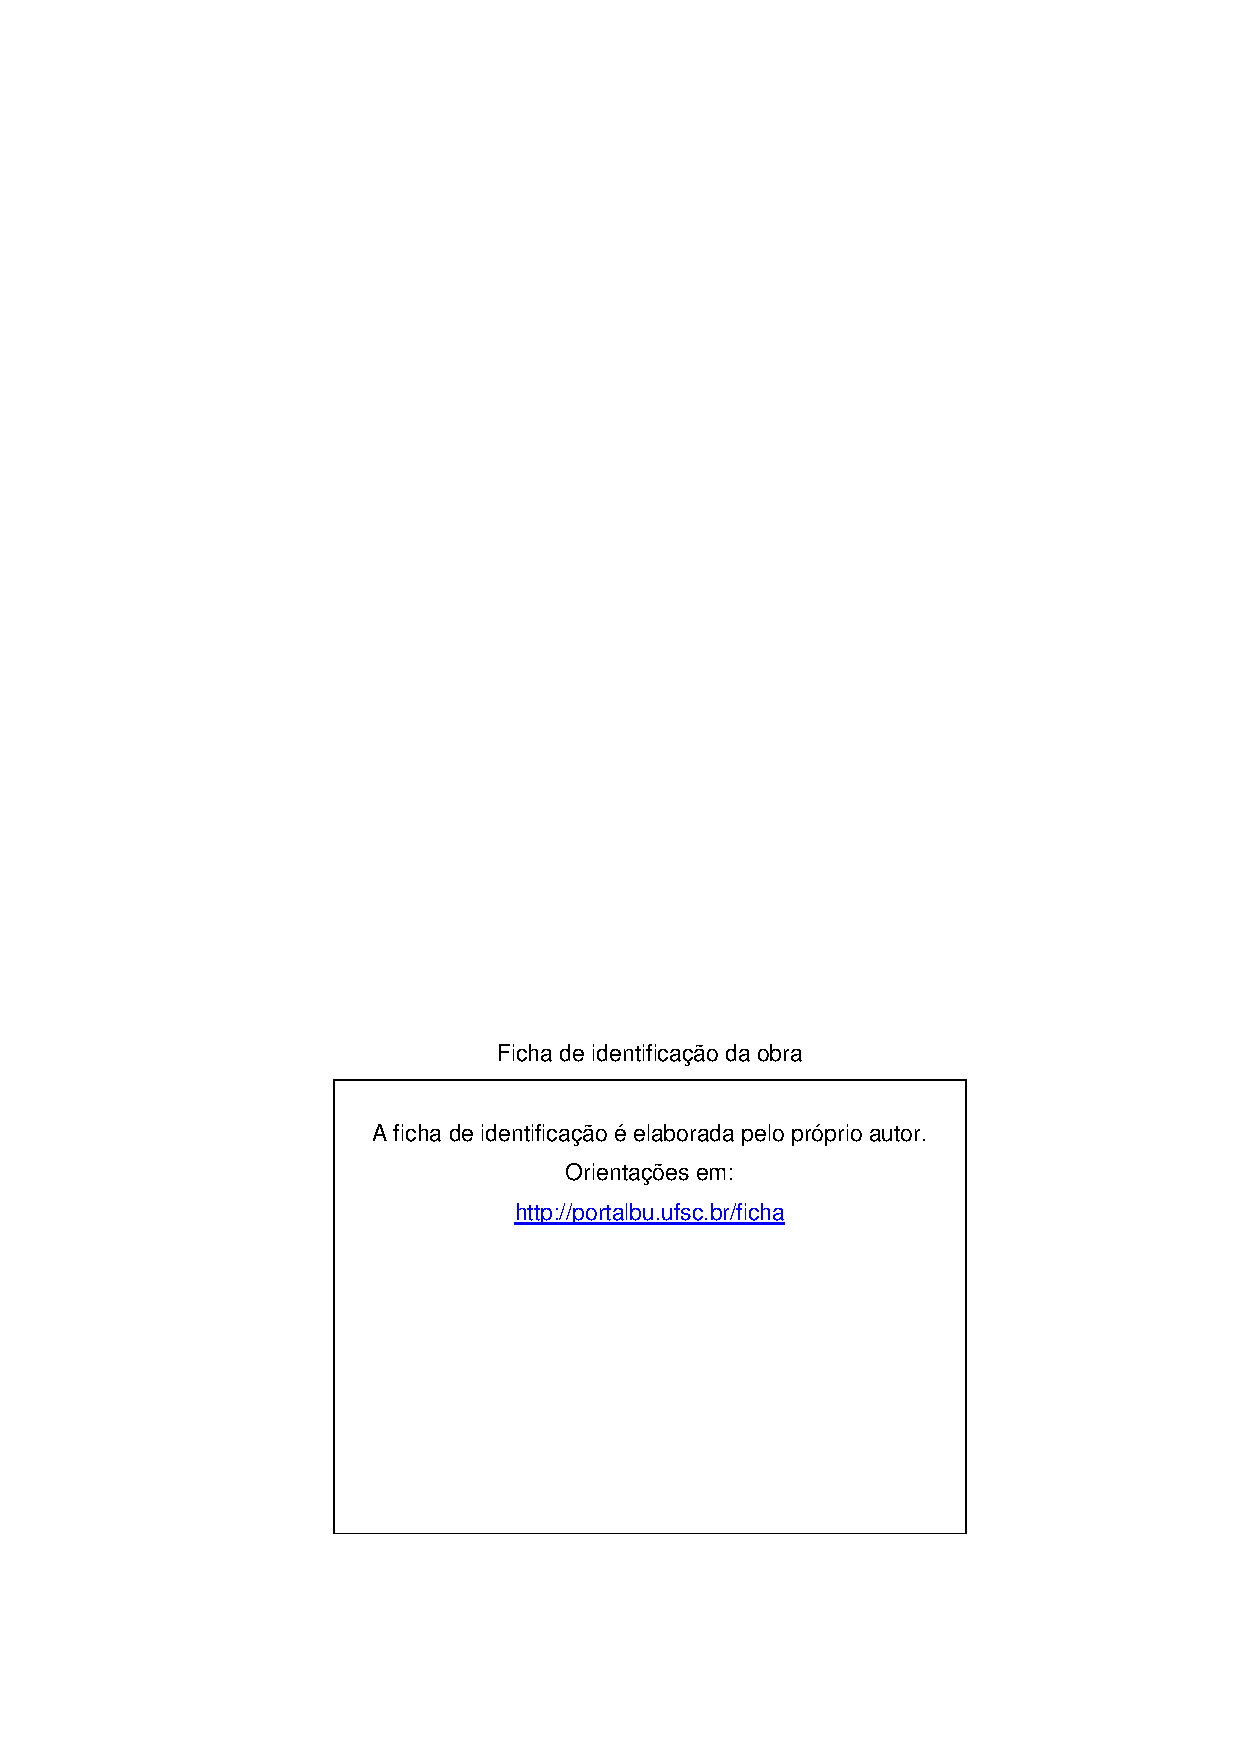
\includepdf{pre/Ficha_Catalografica.pdf}
%\end{fichacatalografica}

%Utilize este arquivo de ficha catalografica
%\begin{fichacatalografica}
\vspace*{12cm} % Posi��o vertical
%\hrule % Linha horizontal

\begin{center} % Minipage Centralizado
\small{\textbf{\cip}}
\framebox[120mm]{%Inicio da caixa
\begin{minipage}{105mm} % Largura [c]{12.5cm}
\begin{flushleft}
\codnome
\end{flushleft}
\MakeUppercase{\sobrenome},~\nome
%\tituloprincipal %\imprimirtitulo

\hspace{0.5cm} \tituloprincipal. / \nome~\sobrenome~ --~ %\imprimirautor
\imprimirlocal:~\sigla,~\imprimirano.\\

\hspace{0.5cm} \pageref{LastPage} p. : il.~color.~;~30 cm.\\

\hspace{0.5cm} \imprimirorientadorRotulo:~ \imprimirorientador.\\

\hspace{0.5cm} \imprimircoorientadorRotulo:~ \imprimircoorientador.\\

\hspace{0.5cm}
\parbox[t]{\textwidth}{\tcc~--~\imprimirinstituicao,~\campus~--~\imprimirprograma,~\imprimirano.}\\

\hspace{0.5cm}
1. \palavrachaveum.
2. \palavrachavedois.
3. \palavrachavetres.
4. \palavrachavequatro.
5. \palavrachavecinco.
I. \MakeUppercase{\sobrenomorient},~\nomorient~\sigorient..
II. \MakeUppercase{\sobrenomcoorient},~\nomcoorient~\sigcoorient..
%II. Universidade xxx.
%III. Faculdade de xxx.
III. T\'itulo.\\

%\hspace{7.75cm} \cdu\\
\begin{flushright}
    						\cdu
\end{flushright}%
%\hspace{8.75cm}
\end{minipage}
}%Fim caixa
\par
\vspace{0.1cm}
Ficha catalogr\'afica elaborada pelo bibliotec\'ario~\bibliotecario~\cbr
\par
Biblioteca Clarice Lispector
\par
\imprimirinstituicao
\par
\campus%Campus: An\'apolis

\end{center}

%\hrule
\end{fichacatalografica}%Retirando ficha catalografica

%----------------------------------------------


% ---
% Inserir folha de aprovação
% ---
%\includepdf[pages={1-2}]{arquivo.pdf}%utilizando duas paginas
%\includepdf[pages={5}, fitpaper=true]{Flauberth__Duarte_TCC.pdf}.
%\begin{folhadeaprovacao}
	\OnehalfSpacing
	\centering
	\imprimirautor\\%
	\vspace*{10pt}		
	\textbf{\imprimirtitulo}%
	\ifnotempty{\imprimirsubtitulo}{~\imprimirsubtitulo}\\%
	%		\vspace*{31.5pt}%3\baselineskip
	\vspace*{\baselineskip}
	%\begin{minipage}{\textwidth}
	% ~do~\imprimirprograma~do~\imprimircentro~da~\imprimirinstituicao~para~a~obtencao~do~t�tulo~de~\imprimirformacao.
	Este~\imprimirtipotrabalho~foi julgado adequado para obten\c{c}\~ao do T\'itulo de ''\imprimirformacao'' e aprovado em sua forma final pelo~\imprimirprograma. \\
		\vspace*{\baselineskip}
	\imprimirlocal, \imprimirdata. \\
	\vspace*{2\baselineskip}
	\assinatura{\OnehalfSpacing\imprimircoordenador \\ \imprimircoordenadorRotulo~do Curso}
	\vspace*{2\baselineskip}
	\textbf{Banca Examinadora:} \\
	\vspace*{\baselineskip}
	\assinatura{\OnehalfSpacing\imprimirorientador \\ \imprimirorientadorRotulo}
	%\end{minipage}%
%	\vspace*{\baselineskip}
%	\assinatura{Prof.\avaliadorinterno, \tituloavaliadorinterno\\ %Nao esta funcionando, ou seja, n�o faz altera�ao
%	Avaliador(\textsuperscript{o}) \\
%	Institui\c{c}\~ao xxxx}

%	\vspace*{\baselineskip}
%	\assinatura{Prof\textsuperscript{a}. \avaliadorexterno, Dr\textsuperscript{a}.\\%Nao esta funcionando, ou seja, n�o faz altera�ao
%	Avaliador(\textsuperscript{a}) \\
%	Institui\c{c}\~ao xxxx}


\end{folhadeaprovacao}
% ---%Retirando 


%---------------------------------------------------
\begin{folhaaprovacao}
    % As assinaturas dos avaliadores entram aqui (as outras já são automáticas)
    \vspace*{\baselineskip}
    \assinatura{Prof.\masculino~\avaliadorinterno, \tituloavaliadorinterno\\
    \avalinterno \\
    \entidadeinterna~(\siglainterno)}

    \vspace*{\baselineskip}
    \assinatura{Prof.\feminino~\avaliadorexterno, \tituloavaliadorexterno\\
    \avalexterno \\
    \entidadeexterna~(\siglaexterno)}
\end{folhaaprovacao}


%---------------------------------------------------

% ---
% Inserir folha de ata da seção pública de tcc
% ---
%\includepdf[pages={5}, fitpaper=true]{folhaDeAta.pdf}.
%% Altera o espa�amento para 1.5 apenas nesta p�gina
%\renewcommand{\baselinestretch}{1.5}\selectfont
%\linespread{0.90}%0.87
\linespread{0.87}\selectfont

%--------Cabe�alho do documento
\noindent\begin{minipage}[c][1.5cm][c]{3.5cm}
%\includegraphics[height=1.5cm]{./figuras/logoEvangelica.eps}

\includegraphics[width=1.5 \textwidth]{./outros/fig/IFGAnapolisHor2.png}
\end{minipage}\quad\quad\quad\qquad
\begin{minipage}{12cm}%10cm
\scriptsize\textbf{\ministerio}\\%\sc
\textbf{\secretaria}\\
\textbf{\instituto}\\
\textbf{\reitoria}\\
\end{minipage}
\vspace{1cm}
%---------------------------------------------------------------------------------------


\begin{center}
	\textbf{ATA N\textsuperscript{o} 20/\imprimirano}\\
	\footnotesize{\MakeUppercase{\textbf{Ata da sess\~ao p\'ublica de apresenta\c{c}\~ao do \imprimirtipotrabalho}}}
\end{center}
\vspace{1.0cm}
\noindent Aos~0\diaata~dias do m\^es de~\mesata~do ano de dois mil e vinte e cinco, \'as~\hinicial~horas, por meio de webconfer\^encia utilizando Google Meet, foi realizada a sess\~ao p\'ublica de apresenta\c{c}\~ao do \imprimirtipotrabalho~do Graduando~\textbf{\alunonome~\alunosobre}~(matr\'icula~\matricula) do~\imprimirprograma. A banca foi composta pelos seguintes membros:~\orientadora,~\membroum,~\membrodois, sob a presid\^encia da primeira. O \imprimirtipotrabalho~tem como t\'itulo ``\textbf{\titulo}'', sob orienta\c{c}\~ao da Prof\textsuperscript{a}~\orientadora. Ap\'os a apresenta\c{c}\~ao do \imprimirtipotrabalho, tendo sido o autor arguido pela Banca Examinadora, a nota obtida foi~\notanumerico~(\notaextenso).
\\
\\
\noindent Encerra-se a presente sess\~ao \'as~\hfinal~horas~e~\mfinal~minutos. Eu Prof\textsuperscript{a}.~\orientadora, dato e assino a presente ata que segue assinada por todos os membros da Banca e pelo graduando.
\vspace{1.0cm}
\small{
\begin{center}
\begin{tabular}{c}
\multicolumn{1}{c}{\asseletronica} \\ 
\multicolumn{1}{c}{Prof\textsuperscript{a}~\orientadora} \\ 
\multicolumn{1}{c}{} \\ 
\asseletronica \\ 
\multicolumn{1}{c}{Prof\textsuperscript{a}~\membroum~} \\ 
\multicolumn{1}{c}{~} \\ 
\asseletronica\\
%\includegraphics[width=0.30 \textwidth]{./outros/fig/AssDaniel.jpg} \\ %\hrulefill comando para linha
\multicolumn{1}{c}{Prof\textsuperscript{a}~\membrodois~} \\ 
\multicolumn{1}{c}{~} \\ 

\includegraphics[width=0.25 \textwidth]{./outros/fig/minhaAssinatura2.png} \\
\multicolumn{1}{c}{\textbf{\alunonome~\alunosobre}} \\
\multicolumn{1}{c}{(Graduando)} \\
\multicolumn{1}{c}{~} \\ 
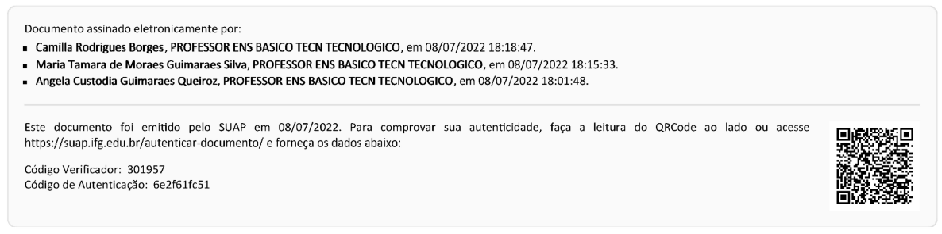
\includegraphics[width=0.97 \textwidth]{./outros/fig/QR_CODE_V2.pdf}
\\
\end{tabular}
\end{center}
}

% Restaura o espa�amento original para as pr�ximas p�ginas
%\renewcommand{\baselinestretch}{1.3}\selectfont
\linespread{1.3}\selectfont

\newpage%Retirando 

%---------------------------------------------------
\begin{comment}%Retire este comentario para aparecer a ata
%---------------------------------------------------
\begin{atareuniao}
\noindent Aos~\diaata~dias do mês de~\mesata~do ano de dois mil e vinte e cinco, às~\hinicial~horas, por meio de webconferência utilizando Google Meet, foi realizada a sessão pública de apresentação do \imprimirtipotrabalho~do Graduando~\textbf{\alunonome~\alunosobre}~(matrícula~\matricula) do~\imprimirprograma. A banca foi composta pelos seguintes membros:~\orientadora,~\avaliadorinterno,~\avaliadorexterno, sob a presidência da primeira. O \imprimirtipotrabalho~tem como título ``\textbf{\titulo}'', sob orientação da Prof\textsuperscript{a}~\orientadora. Após a apresentação do \imprimirtipotrabalho, tendo sido o autor arguido pela Banca Examinadora, a nota obtida foi~\notanumerico~(\notaextenso).

\vspace{0.5cm}
\noindent Encerra-se a presente sessão às~\hfinal~horas~e~\mfinal~minutos. Eu Prof\textsuperscript{a}.~\orientadora, dato e assino a presente ata que segue assinada por todos os membros da Banca e pelo graduando.

\vspace{0.1cm}
\vspace{-0.1cm} % Espaço negativo para "puxar" a tabela para cima
{\footnotesize 
\begin{center}
    % Ajusta o respiro global da tabela
    \renewcommand{\arraystretch}{0.8} 
    \begin{tabular}{c}
        \asseletronica \\[0.2cm] % <--- Adiciona 0.2cm de espaço APENAS aqui
        Prof\textsuperscript{a}~\orientadora \\[0.4cm] % Espaço maior entre pessoas
        
        \asseletronica \\[0.2cm]
        Prof\textsuperscript{a}~\avaliadorinterno \\[0.4cm] 
        
        \asseletronica \\[0.2cm]
        Prof\textsuperscript{a}~\avaliadorexterno \\[0.4cm] 
        
        
\includegraphics[width=0.20\textwidth]{./outros/fig/minhaAssinatura2.png} \\[0.1cm]
        \textbf{\alunonome~\alunosobre} \\
        (Graduando) \\[0.3cm] 
        
        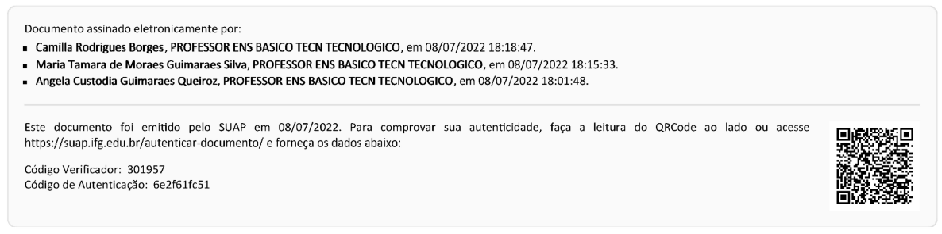
\includegraphics[width=0.79\textwidth]{./outros/fig/QR_CODE_V2.pdf}
    \end{tabular}
\end{center}
}
\end{atareuniao}
%---------------------------------------------------
\end{comment}
%---------------------------------------------------

% --------------------------------------------------
% Inserir folha de autorização para disponibilização
% --------------------------------------------------
%\linespread{0.87}\selectfont
%--------Cabe�alho do documento
\noindent\begin{minipage}[c][1.5cm][c]{3.5cm}

\includegraphics[width=1.5 \textwidth]{./outros/fig/IFGAnapolisHor2.png}
\end{minipage}\quad\quad\quad\qquad
\begin{minipage}{12cm}%10cm
\scriptsize\textbf{\ministerio}\\
\textbf{\secretaria}\\
\textbf{\instituto}\\
\textbf{\MakeTextUppercase{\campus}}\\
\textbf{\biblioteca}\\
\end{minipage}
%\vspace{-0.1cm}
\small{
\begin{center}
	\termo
\end{center}

\termodois

\noindent \textbf{Identifica\c{c}\~ao de Produ\c{c}\~ao T\'ecnico-Cient\'ifica}

\begin{tabular}{lllll}
\lbrack ~~\rbrack & Tese &  & \lbrack ~~\rbrack & Artigo Cient\'ifico \\ 
\lbrack ~~\rbrack & Disserta\c{c}\~ao &  & \lbrack ~~\rbrack & Cap\'itulo de Livro \\ 
\lbrack ~~\rbrack & Monografia -- Especializa\c{c}\~ao &  & \lbrack ~~\rbrack & Livro \\ 
\lbrack X\rbrack & TCC -- Gradua\c{c}\~ao &  & \lbrack ~~\rbrack & Trabalho Apresentado em Evento \\ 
\lbrack ~~\rbrack & Produto T\'ecnico e Educacional -- Tipo: & \multicolumn{3}{l}{\hrulefill} \\ 
\end{tabular}

\quad

\noindent Nome Completo do Autor:~\textbf{\alunonome~\alunosobre}

\noindent Matr\'icula:~\textbf{\matricula}

\noindent T\'ituto do Trabalho:~\textbf{\tituloprincipal}

\noindent \textbf{Autoriza\c{c}\~ao -- Marque uma das op\c{c}\~oes}

\begin{enumerate}
	\item (X) Autorizo disponibilizar meu trabalho no Reposit\'orio Digital do IFG (acesso aberto);
	\item (~) Autorizo disponibilizar meu trabalho no Reposit\'orio Digital do IFG somente ap\'os a data 20/10/20 (Embargo);
	\item (~) N\~ao autorizo disponibilizar meu trabalho no Reposit\'orio Digital do IFG (acesso restrito)
\end{enumerate}

\noindent Ao indicar a op\c{c}\~ao \textbf{2 ou 3}, marque a justificativa:
\begin{description}
	\item[(~~)] O documento est\'a sujeito a registro de patente.
	\item[(~~)] O documento pode vir a ser publicado como livro, cap\'itulo de livro ou artigo.
	\item[(~~)] Outra justificativa: \hrulefill
\end{description}

\begin{center}
	\textbf{\declaracao}
\end{center}

\noindent O(A) referido(a) autor(a) declara que:

\textbf{(i)}~o documento \'e seu trabalho original, det\'em os direitos autorais de produ\c{c}\~ao t\'ecnico-cient\'ifica e n\~ao infringe os direitos de qualquer outro pessoa ou entidade;

\textbf{(ii)}~\termotres

\textbf{(iii)}~cumpriu quaisquer obriga\c{c}\~oes exigidas por contrato ou acordo, caso o documento entregue seja baseado em trabalho finaciado ou apoiado por outra institui\c{c}\~ao que n\~ao o \entidade.

%\todaydia
\begin{flushright}
An\'apolis, {\diaata~de~\mesata}~de~{\todayano}
\end{flushright}

\begin{center}
\begin{tabular}{c}

\includegraphics[width=0.19 \textwidth]{./outros/fig/minhaAssinatura2.png} \\ 
\multicolumn{1}{c}{~\alunonome \alunosobre} \\ 
%\multicolumn{1}{c}{\hrulefill} \\ 
\end{tabular}
\end{center}
}%Fim \small

\linespread{1.3}\selectfont
%Retirando 
%\includepdf[pages={5}, fitpaper=true]{folhaTermo.pdf}.
%---------------------------------------------------
\begin{comment}% Descomente para aparecer O Termo de Autorização da biblioteca

\linespread{0.87}\selectfont
%--------Cabeçalho do documento
\noindent\begin{minipage}[c][1.5cm][c]{3.5cm}

\includegraphics[width=1.5 \textwidth]{./outros/fig/IFGAnapolisHor2.png}
\end{minipage}\quad\quad\quad\qquad
\begin{minipage}{12cm}%10cm
\scriptsize\textbf{\ministerio}\\
\textbf{\secretaria}\\
\textbf{\instituto}\\
\textbf{\MakeTextUppercase{\campus}}\\
\textbf{\biblioteca}\\
\end{minipage}
%\vspace{-0.1cm}
\small{
\begin{center}
	\termo
\end{center}

\termodois

\noindent \textbf{Identifica\c{c}\~ao de Produ\c{c}\~ao T\'ecnico-Cient\'ifica}

\begin{tabular}{lllll}
\lbrack ~~\rbrack & Tese &  & \lbrack ~~\rbrack & Artigo Cient\'ifico \\ 
\lbrack ~~\rbrack & Disserta\c{c}\~ao &  & \lbrack ~~\rbrack & Cap\'itulo de Livro \\ 
\lbrack ~~\rbrack & Monografia -- Especializa\c{c}\~ao &  & \lbrack ~~\rbrack & Livro \\ 
\lbrack X\rbrack & TCC -- Gradua\c{c}\~ao &  & \lbrack ~~\rbrack & Trabalho Apresentado em Evento \\ 
\lbrack ~~\rbrack & Produto T\'ecnico e Educacional -- Tipo: & \multicolumn{3}{l}{\hrulefill} \\ 
\end{tabular}

\quad

\noindent Nome Completo do Autor:~\textbf{\alunonome~\alunosobre}

\noindent Matr\'icula:~\textbf{\matricula}

\noindent T\'ituto do Trabalho:~\textbf{\tituloprincipal}

\noindent \textbf{Autoriza\c{c}\~ao -- Marque uma das op\c{c}\~oes}

\begin{enumerate}
	\item (X) Autorizo disponibilizar meu trabalho no Reposit\'orio Digital do IFG (acesso aberto);
	\item (~) Autorizo disponibilizar meu trabalho no Reposit\'orio Digital do IFG somente ap\'os a data 20/10/20 (Embargo);
	\item (~) N\~ao autorizo disponibilizar meu trabalho no Reposit\'orio Digital do IFG (acesso restrito)
\end{enumerate}

\noindent Ao indicar a op\c{c}\~ao \textbf{2 ou 3}, marque a justificativa:
\begin{description}
	\item[(~~)] O documento est\'a sujeito a registro de patente.
	\item[(~~)] O documento pode vir a ser publicado como livro, cap\'itulo de livro ou artigo.
	\item[(~~)] Outra justificativa: \hrulefill
\end{description}

\begin{center}
	\textbf{\declaracao}
\end{center}

\noindent O(A) referido(a) autor(a) declara que:

\textbf{(i)}~o documento \'e seu trabalho original, det\'em os direitos autorais de produ\c{c}\~ao t\'ecnico-cient\'ifica e n\~ao infringe os direitos de qualquer outro pessoa ou entidade;

\textbf{(ii)}~\termotres

\textbf{(iii)}~cumpriu quaisquer obriga\c{c}\~oes exigidas por contrato ou acordo, caso o documento entregue seja baseado em trabalho finaciado ou apoiado por outra institui\c{c}\~ao que n\~ao o \entidade.

%\todaydia
\begin{flushright}
An\'apolis, {\diaata~de~\mesata}~de~{\todayano}
\end{flushright}

\begin{center}
\begin{tabular}{c}

\includegraphics[width=0.19 \textwidth]{./outros/fig/minhaAssinatura2.png} \\ 
\multicolumn{1}{c}{~\alunonome \alunosobre} \\ 
%\multicolumn{1}{c}{\hrulefill} \\ 
\end{tabular}
\end{center}
}%Fim \small

\linespread{1.3}\selectfont

\end{comment}
%---------------------------------------------------


% ---
% Dedicatória
% ---
%\begin{dedicatoria}
%	\vspace*{\fill}
%	\noindent
%	\begin{adjustwidth*}{}{5.5cm}     
%		Este trabalho é dedicado aos meus colegas de %classe e aos meus queridos pais.
%	\end{adjustwidth*}
%\end{dedicatoria}
% ---

% ---
% Agradecimentos
% ---
%\begin{agradecimentos}
%	Inserir os agradecimentos aos colaboradores à %execução do trabalho. 
%\end{agradecimentos}
% ---

% ---
% Epígrafe
% ---
\begin{epigrafe}
    \null\vfill % Cria o ponto no topo e empurra o conteúdo para baixo
		\vspace{3cm}
    \begin{flushright}
        \textit{Se você for receptivo e humilde, a matemática o conduzirá pela mão. Repetidas vezes, quando estive perdido sem saber como prosseguir, bastou-me esperar até sentir que a matemática me guiava pela mão. Ela me conduziu por um caminho inesperado, um caminho onde novas perspectivas se abrem, um caminho que leva a um território novo, onde é possível estabelecer uma base de operações, a partir da qual se pode observar os arredores e planejar o progresso futuro.} \\
        \vspace{0.3cm}
        (Paul Dirac)
    \end{flushright}
    \vspace*{0.5cm} % Garante uma margem mínima do fim da folha (ajuste se quiser mais baixo)
\end{epigrafe}



% ---

% ---
% RESUMOS
% ---

% resumo em português
\setlength{\absparsep}{18pt} % ajusta o espaçamento dos parágrafos do resumo
\begin{resumo}
\SingleSpacing
%Os resultados revelam que não existe uma técnica universalmente superior: o RLM-\textit{subagging} apresentou melhor desempenho para Mn e Ni, o RLM-\textit{bagging} mostrou-se superior para Fe, enquanto a RLM clássica demonstrou desempenho superior para Mo e Cr. O comportamento diferenciado entre os analitos é atribuído à complexidade espectral de cada elemento: o Fe, por apresentar maior densidade de linhas espectrais com potencial de autoabsorção e sobreposições com outros elementos da matriz, beneficia-se da agregação de múltiplos modelos. Em contrapartida, Mn, Mo, Cr e Ni têm sua relação espectral-concentração suficientemente capturada pela RLM clássica ou pelo RLM-\textit{subagging}, sem ganho adicional com o RLM-\textit{bagging}. Todos os modelos apresentaram R$^2$ superior a 0,9815, evidenciando elevada capacidade preditiva. Quanto à eficiência computacional, o RLM-\textit{subagging} mostrou-se em média 3,0 vezes mais rápido que o RLM-\textit{bagging}, configurando-se como alternativa equilibrada entre precisão e eficiência em aplicações quimiométricas sujeitas a restrições temporais.

A calibração multivariada é essencial para determinar a composição elementar de aço-ligas a partir de dados espectrométricos. Este trabalho investigou, em caráter exploratório, a aplicação das técnicas de reamostragem \textit{bootstrap}, \textit{bagging} e \textit{subagging} incorporadas à Regressão Linear Múltipla (RLM) para a estimativa quantitativa dos elementos Manganês (Mn), Molibdênio (Mo), Cromo (Cr), Níquel (Ni) e Ferro (Fe). Paralelamente, conduziu-se a modernização de um sistema legado monolítico em Java \textit{Desktop} para uma aplicação \textit{Web} em Python e Streamlit, adotando arquitetura desacoplada em três módulos de responsabilidade única. A validação do sistema reescrito e a fidelidade a lógica matemática original foram asseguradas por uma suíte de 92 testes automatizados desenvolvida com \texttt{pytest}, englobando 21 testes unitários, 60 testes de caixa-preta baseados nos arquivos do sistema legado e 11 testes de carga e estresse com matrizes de alta dimensão. Os resultados experimentais demonstraram que a eficiência das técnicas de \textit{ensemble} varia conforme o analito: a RLM clássica obteve menor \textit{Root-Mean-Square Error of Prediction} (RMSEP) para o Molibdênio e o Cromo; o RLM-\textit{bagging} obteve menor erro para o Ferro; e o RLM-\textit{subagging} apresentou melhor desempenho para o Manganês e o Níquel (neste último, com desempenho numericamente equivalente ao da RLM clássica, com diferença de 0,25\% no (RMSEP). Em termos de eficiência computacional, o RLM-\textit{subagging} reduziu o tempo de processamento em relação ao RLM-\textit{bagging} em quatro dos cinco analitos. A suíte de testes confirmou a equivalência numérica estrita para os métodos determinísticos e a estabilidade da aplicação sob exigência computacional elevada, comprovando a viabilidade da modernização arquitetural sem perda de acurácia científica.

\textbf{Palavras-chave}: \palavrachaveum. \palavrachavedois. \palavrachavetres. \palavrachavequatro. \palavrachavecinco.
\end{resumo}

% resumo em inglês
\begin{resumo}[Abstract]
\SingleSpacing
\begin{otherlanguage*}{english}
%---------------------------------------------------
%The results reveal that no universally superior technique exists: RLM-\textit{subagging} achieved the best performance for Mn and Ni, RLM-\textit{bagging} proved superior for Fe, while classical MLR demonstrated superior performance for Mo and Cr. The differentiated behavior among analytes is attributed to the spectral complexity of each element: Fe, due to its higher density of spectral lines with self-absorption potential and overlaps with other matrix elements, benefits from the aggregation of multiple models. In contrast, Mn, Mo, Cr and Ni have their spectral-concentration relationship sufficiently captured by classical MLR or MLR-\textit{subagging}, with no additional gain from MLR-\textit{bagging}. All models presented R$^2$ values above 0.9815, evidencing high predictive capacity. Regarding computational efficiency, MLR-\textit{subagging} proved on average 3.0 times faster than MLR-\textit{bagging}, establishing itself as a balanced alternative between accuracy and efficiency in chemometric applications subject to time constraints.
%------------------------

Multivariate calibration is essential for determining the elemental composition of alloy steels from spectrometric data. This study explored the application of bootstrap resampling, bagging, and subagging techniques incorporated into Multiple Linear Regression (MLR) for the quantitative estimation of Manganese (Mn), Molybdenum (Mo), Chromium (Cr), Nickel (Ni), and Iron (Fe). Concurrently, a legacy monolithic Java Desktop system was modernized into a Python and Streamlit Web application, adopting a decoupled architecture structured into three single-responsibility modules. The validation of the rewritten system and its fidelity to the original algorithmic core were ensured by a suite of 92 automated tests developed with pytest, encompassing 21 unit tests, 60 black-box tests based on legacy system outputs, and 11 load and stress tests with high-dimensional matrices. Experimental results demonstrated that the efficiency of ensemble techniques varies depending on the analyte: classical MLR achieved a lower Root-Mean-Square Error of Prediction (RMSEP) for Molybdenum and Chromium; MLR-bagging yielded the lowest error for Iron; and MLR-subagging exhibited superior performance for Manganese and Nickel (in the latter, with performance numerically equivalent to classical MLR, showing a 0.25\% difference in RMSEP). In terms of computational efficiency, MLR-subagging reduced processing time compared to MLR-bagging across four of the five analytes. The test suite confirmed strict numerical equivalence for deterministic methods and application stability under high computational demand, proving the feasibility of architectural modernization without loss of scientific accuracy.%


%------------------------

\textbf{Keywords}: Resampling. Multivariate Calibration. Bagging. Subagging. Chemometrics.
\end{otherlanguage*}
\end{resumo}

%% resumo em francês 
%\begin{resumo}[Résumé]
% \begin{otherlanguage*}{french}
%    Il s'agit d'un résumé en français.
% 
%   \textbf{Mots-clés}: latex. abntex. publication de textes.
% \end{otherlanguage*}
%\end{resumo}
%
%% resumo em espanhol
%\begin{resumo}[Resumen]
% \begin{otherlanguage*}{spanish}
%   Este es el resumen en español.
%  
%   \textbf{Palabras clave}: latex. abntex. publicación de textos.
% \end{otherlanguage*}
%\end{resumo}
%% ---

{%hidelinks
	\hypersetup{hidelinks}
	% ---
	% inserir lista de ilustrações
	% ---
	\pdfbookmark[0]{\listfigurename}{lof}
	\listoffigures* %Retirado
	\cleardoublepage
	% ---
	
	% ---
	% inserir lista de quadros
	% ---
	\pdfbookmark[0]{\listofquadrosname}{loq}
	\listofquadros* %Retirado
	\cleardoublepage
	% ---
	
	% ---
	% inserir lista de tabelas
	% ---
	\pdfbookmark[0]{\listtablename}{lot}
	\listoftables* %Retirando
	\cleardoublepage
	% ---
	
	% ---
	% inserir lista de abreviaturas e siglas (devem ser declarados no preambulo)
	% ---

\imprimirlistadesiglas %Retirando
%\cleardoublepage
	% ---
	
	% ---
	% inserir lista de símbolos (devem ser declarados no preambulo)
	% ---
\imprimirlistadesimbolos %Retirando
%\cleardoublepage
	% ---
	
	% ---
	% inserir o sumario
	% ---
	\pdfbookmark[0]{\contentsname}{toc}
	\tableofcontents*
	\cleardoublepage
	
}%hidelinks
% ---
%------utilizado
%% ---
% Capa
% ---
\imprimircapa
% ---

% ---
% Folha de rosto
% (o * indica que haverá a ficha catalográfica)
% ---
\imprimirfolhaderosto
% ---

% ---
% Ficha Catalografica em pdf e código
% 
% ---

%\begin{fichacatalografica}
%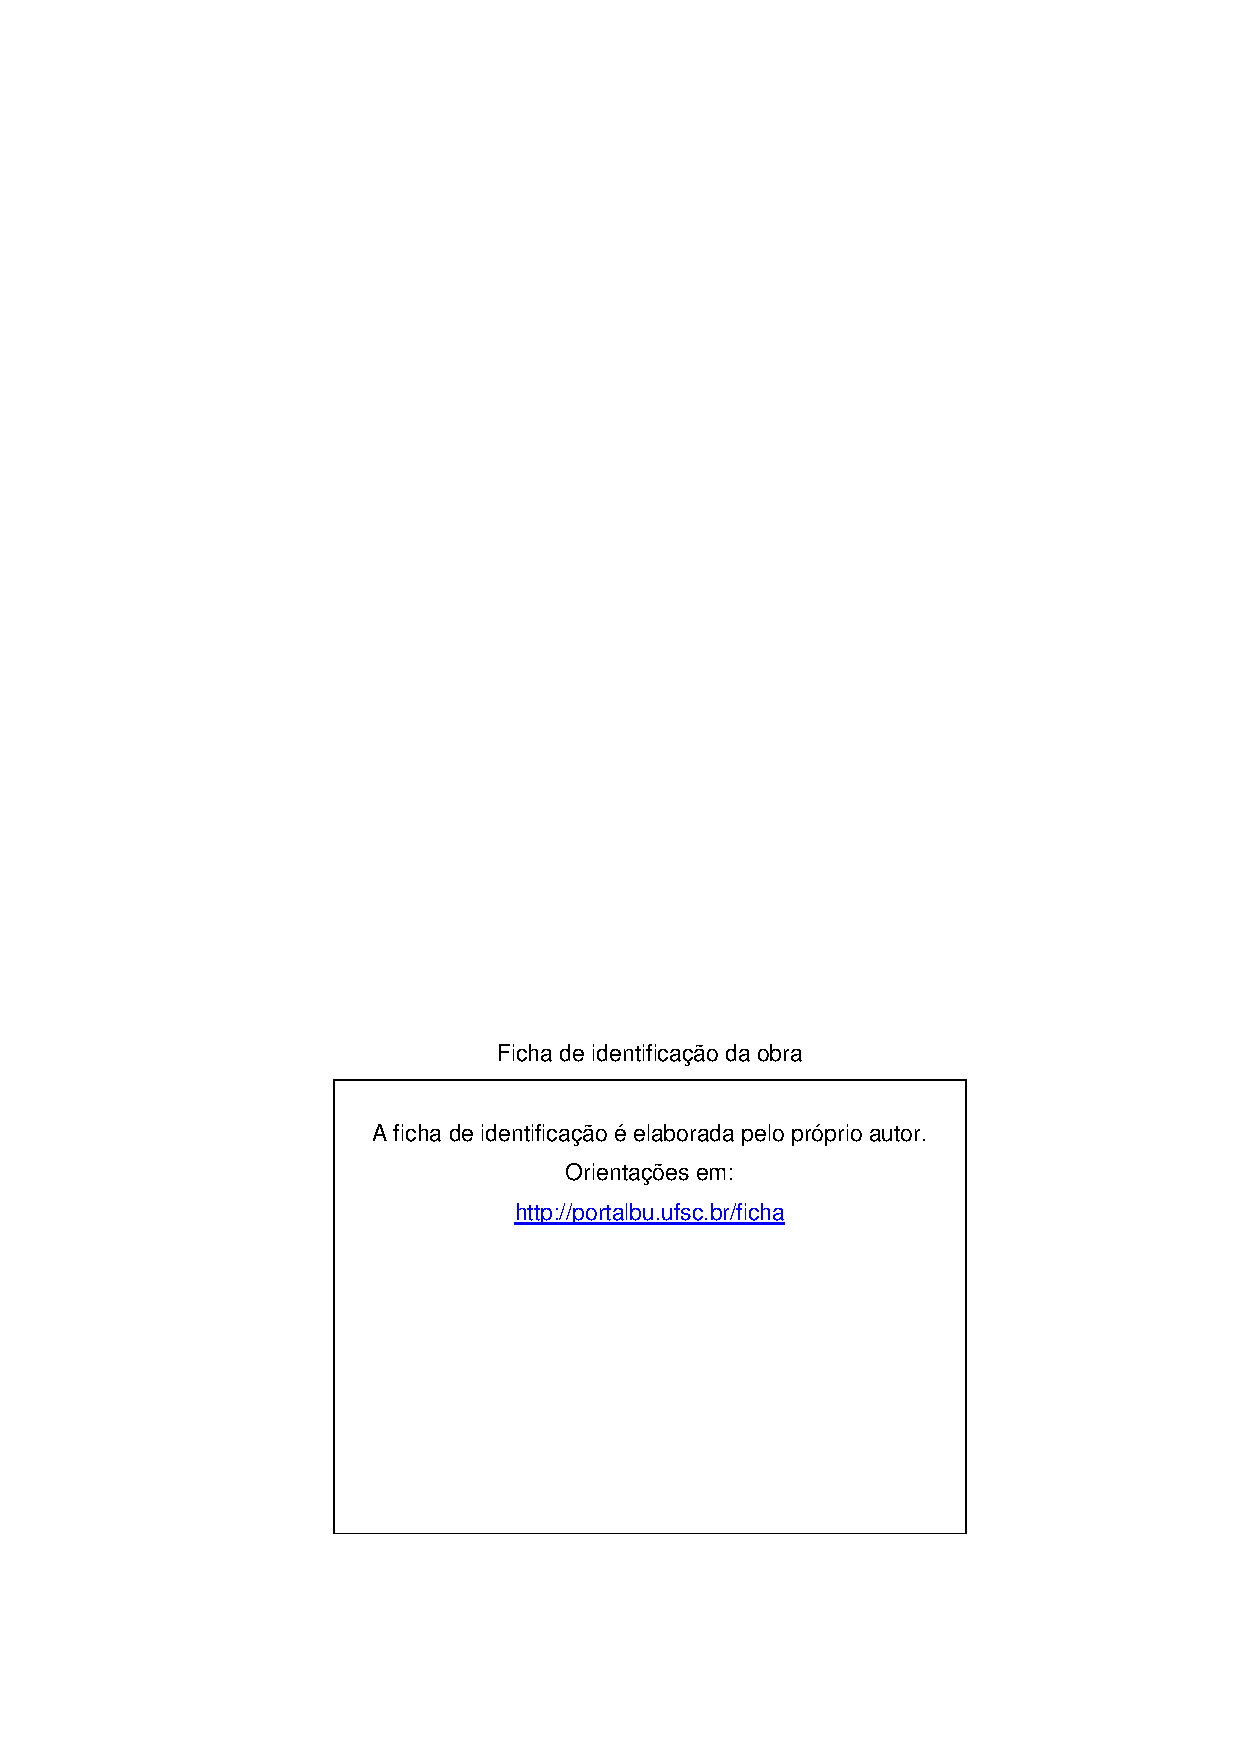
\includepdf{pre/Ficha_Catalografica.pdf}
%\end{fichacatalografica}

%Utilize este arquivo de ficha catalografica
%\begin{fichacatalografica}
\vspace*{12cm} % Posi��o vertical
%\hrule % Linha horizontal

\begin{center} % Minipage Centralizado
\small{\textbf{\cip}}
\framebox[120mm]{%Inicio da caixa
\begin{minipage}{105mm} % Largura [c]{12.5cm}
\begin{flushleft}
\codnome
\end{flushleft}
\MakeUppercase{\sobrenome},~\nome
%\tituloprincipal %\imprimirtitulo

\hspace{0.5cm} \tituloprincipal. / \nome~\sobrenome~ --~ %\imprimirautor
\imprimirlocal:~\sigla,~\imprimirano.\\

\hspace{0.5cm} \pageref{LastPage} p. : il.~color.~;~30 cm.\\

\hspace{0.5cm} \imprimirorientadorRotulo:~ \imprimirorientador.\\

\hspace{0.5cm} \imprimircoorientadorRotulo:~ \imprimircoorientador.\\

\hspace{0.5cm}
\parbox[t]{\textwidth}{\tcc~--~\imprimirinstituicao,~\campus~--~\imprimirprograma,~\imprimirano.}\\

\hspace{0.5cm}
1. \palavrachaveum.
2. \palavrachavedois.
3. \palavrachavetres.
4. \palavrachavequatro.
5. \palavrachavecinco.
I. \MakeUppercase{\sobrenomorient},~\nomorient~\sigorient..
II. \MakeUppercase{\sobrenomcoorient},~\nomcoorient~\sigcoorient..
%II. Universidade xxx.
%III. Faculdade de xxx.
III. T\'itulo.\\

%\hspace{7.75cm} \cdu\\
\begin{flushright}
    						\cdu
\end{flushright}%
%\hspace{8.75cm}
\end{minipage}
}%Fim caixa
\par
\vspace{0.1cm}
Ficha catalogr\'afica elaborada pelo bibliotec\'ario~\bibliotecario~\cbr
\par
Biblioteca Clarice Lispector
\par
\imprimirinstituicao
\par
\campus%Campus: An\'apolis

\end{center}

%\hrule
\end{fichacatalografica}%Retirando ficha catalografica

%----------------------------------------------


% ---
% Inserir folha de aprovação
% ---
%\includepdf[pages={1-2}]{arquivo.pdf}%utilizando duas paginas
%\includepdf[pages={5}, fitpaper=true]{Flauberth__Duarte_TCC.pdf}.
%\begin{folhadeaprovacao}
	\OnehalfSpacing
	\centering
	\imprimirautor\\%
	\vspace*{10pt}		
	\textbf{\imprimirtitulo}%
	\ifnotempty{\imprimirsubtitulo}{~\imprimirsubtitulo}\\%
	%		\vspace*{31.5pt}%3\baselineskip
	\vspace*{\baselineskip}
	%\begin{minipage}{\textwidth}
	% ~do~\imprimirprograma~do~\imprimircentro~da~\imprimirinstituicao~para~a~obtencao~do~t�tulo~de~\imprimirformacao.
	Este~\imprimirtipotrabalho~foi julgado adequado para obten\c{c}\~ao do T\'itulo de ''\imprimirformacao'' e aprovado em sua forma final pelo~\imprimirprograma. \\
		\vspace*{\baselineskip}
	\imprimirlocal, \imprimirdata. \\
	\vspace*{2\baselineskip}
	\assinatura{\OnehalfSpacing\imprimircoordenador \\ \imprimircoordenadorRotulo~do Curso}
	\vspace*{2\baselineskip}
	\textbf{Banca Examinadora:} \\
	\vspace*{\baselineskip}
	\assinatura{\OnehalfSpacing\imprimirorientador \\ \imprimirorientadorRotulo}
	%\end{minipage}%
%	\vspace*{\baselineskip}
%	\assinatura{Prof.\avaliadorinterno, \tituloavaliadorinterno\\ %Nao esta funcionando, ou seja, n�o faz altera�ao
%	Avaliador(\textsuperscript{o}) \\
%	Institui\c{c}\~ao xxxx}

%	\vspace*{\baselineskip}
%	\assinatura{Prof\textsuperscript{a}. \avaliadorexterno, Dr\textsuperscript{a}.\\%Nao esta funcionando, ou seja, n�o faz altera�ao
%	Avaliador(\textsuperscript{a}) \\
%	Institui\c{c}\~ao xxxx}


\end{folhadeaprovacao}
% ---%Retirando 


%---------------------------------------------------
\begin{folhaaprovacao}
    % As assinaturas dos avaliadores entram aqui (as outras já são automáticas)
    \vspace*{\baselineskip}
    \assinatura{Prof.\masculino~\avaliadorinterno, \tituloavaliadorinterno\\
    \avalinterno \\
    \entidadeinterna~(\siglainterno)}

    \vspace*{\baselineskip}
    \assinatura{Prof.\feminino~\avaliadorexterno, \tituloavaliadorexterno\\
    \avalexterno \\
    \entidadeexterna~(\siglaexterno)}
\end{folhaaprovacao}


%---------------------------------------------------

% ---
% Inserir folha de ata da seção pública de tcc
% ---
%\includepdf[pages={5}, fitpaper=true]{folhaDeAta.pdf}.
%% Altera o espa�amento para 1.5 apenas nesta p�gina
%\renewcommand{\baselinestretch}{1.5}\selectfont
%\linespread{0.90}%0.87
\linespread{0.87}\selectfont

%--------Cabe�alho do documento
\noindent\begin{minipage}[c][1.5cm][c]{3.5cm}
%\includegraphics[height=1.5cm]{./figuras/logoEvangelica.eps}

\includegraphics[width=1.5 \textwidth]{./outros/fig/IFGAnapolisHor2.png}
\end{minipage}\quad\quad\quad\qquad
\begin{minipage}{12cm}%10cm
\scriptsize\textbf{\ministerio}\\%\sc
\textbf{\secretaria}\\
\textbf{\instituto}\\
\textbf{\reitoria}\\
\end{minipage}
\vspace{1cm}
%---------------------------------------------------------------------------------------


\begin{center}
	\textbf{ATA N\textsuperscript{o} 20/\imprimirano}\\
	\footnotesize{\MakeUppercase{\textbf{Ata da sess\~ao p\'ublica de apresenta\c{c}\~ao do \imprimirtipotrabalho}}}
\end{center}
\vspace{1.0cm}
\noindent Aos~0\diaata~dias do m\^es de~\mesata~do ano de dois mil e vinte e cinco, \'as~\hinicial~horas, por meio de webconfer\^encia utilizando Google Meet, foi realizada a sess\~ao p\'ublica de apresenta\c{c}\~ao do \imprimirtipotrabalho~do Graduando~\textbf{\alunonome~\alunosobre}~(matr\'icula~\matricula) do~\imprimirprograma. A banca foi composta pelos seguintes membros:~\orientadora,~\membroum,~\membrodois, sob a presid\^encia da primeira. O \imprimirtipotrabalho~tem como t\'itulo ``\textbf{\titulo}'', sob orienta\c{c}\~ao da Prof\textsuperscript{a}~\orientadora. Ap\'os a apresenta\c{c}\~ao do \imprimirtipotrabalho, tendo sido o autor arguido pela Banca Examinadora, a nota obtida foi~\notanumerico~(\notaextenso).
\\
\\
\noindent Encerra-se a presente sess\~ao \'as~\hfinal~horas~e~\mfinal~minutos. Eu Prof\textsuperscript{a}.~\orientadora, dato e assino a presente ata que segue assinada por todos os membros da Banca e pelo graduando.
\vspace{1.0cm}
\small{
\begin{center}
\begin{tabular}{c}
\multicolumn{1}{c}{\asseletronica} \\ 
\multicolumn{1}{c}{Prof\textsuperscript{a}~\orientadora} \\ 
\multicolumn{1}{c}{} \\ 
\asseletronica \\ 
\multicolumn{1}{c}{Prof\textsuperscript{a}~\membroum~} \\ 
\multicolumn{1}{c}{~} \\ 
\asseletronica\\
%\includegraphics[width=0.30 \textwidth]{./outros/fig/AssDaniel.jpg} \\ %\hrulefill comando para linha
\multicolumn{1}{c}{Prof\textsuperscript{a}~\membrodois~} \\ 
\multicolumn{1}{c}{~} \\ 

\includegraphics[width=0.25 \textwidth]{./outros/fig/minhaAssinatura2.png} \\
\multicolumn{1}{c}{\textbf{\alunonome~\alunosobre}} \\
\multicolumn{1}{c}{(Graduando)} \\
\multicolumn{1}{c}{~} \\ 
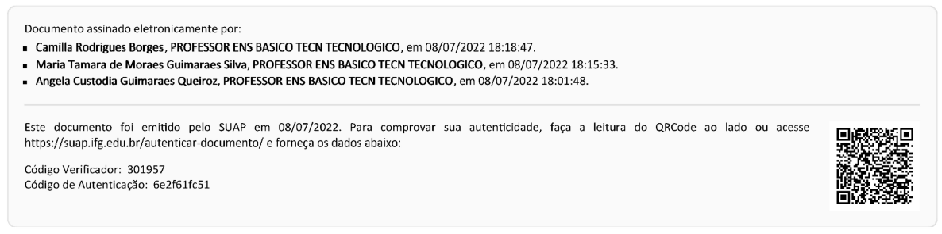
\includegraphics[width=0.97 \textwidth]{./outros/fig/QR_CODE_V2.pdf}
\\
\end{tabular}
\end{center}
}

% Restaura o espa�amento original para as pr�ximas p�ginas
%\renewcommand{\baselinestretch}{1.3}\selectfont
\linespread{1.3}\selectfont

\newpage%Retirando 

%---------------------------------------------------
\begin{comment}%Retire este comentario para aparecer a ata
%---------------------------------------------------
\begin{atareuniao}
\noindent Aos~\diaata~dias do mês de~\mesata~do ano de dois mil e vinte e cinco, às~\hinicial~horas, por meio de webconferência utilizando Google Meet, foi realizada a sessão pública de apresentação do \imprimirtipotrabalho~do Graduando~\textbf{\alunonome~\alunosobre}~(matrícula~\matricula) do~\imprimirprograma. A banca foi composta pelos seguintes membros:~\orientadora,~\avaliadorinterno,~\avaliadorexterno, sob a presidência da primeira. O \imprimirtipotrabalho~tem como título ``\textbf{\titulo}'', sob orientação da Prof\textsuperscript{a}~\orientadora. Após a apresentação do \imprimirtipotrabalho, tendo sido o autor arguido pela Banca Examinadora, a nota obtida foi~\notanumerico~(\notaextenso).

\vspace{0.5cm}
\noindent Encerra-se a presente sessão às~\hfinal~horas~e~\mfinal~minutos. Eu Prof\textsuperscript{a}.~\orientadora, dato e assino a presente ata que segue assinada por todos os membros da Banca e pelo graduando.

\vspace{0.1cm}
\vspace{-0.1cm} % Espaço negativo para "puxar" a tabela para cima
{\footnotesize 
\begin{center}
    % Ajusta o respiro global da tabela
    \renewcommand{\arraystretch}{0.8} 
    \begin{tabular}{c}
        \asseletronica \\[0.2cm] % <--- Adiciona 0.2cm de espaço APENAS aqui
        Prof\textsuperscript{a}~\orientadora \\[0.4cm] % Espaço maior entre pessoas
        
        \asseletronica \\[0.2cm]
        Prof\textsuperscript{a}~\avaliadorinterno \\[0.4cm] 
        
        \asseletronica \\[0.2cm]
        Prof\textsuperscript{a}~\avaliadorexterno \\[0.4cm] 
        
        
\includegraphics[width=0.20\textwidth]{./outros/fig/minhaAssinatura2.png} \\[0.1cm]
        \textbf{\alunonome~\alunosobre} \\
        (Graduando) \\[0.3cm] 
        
        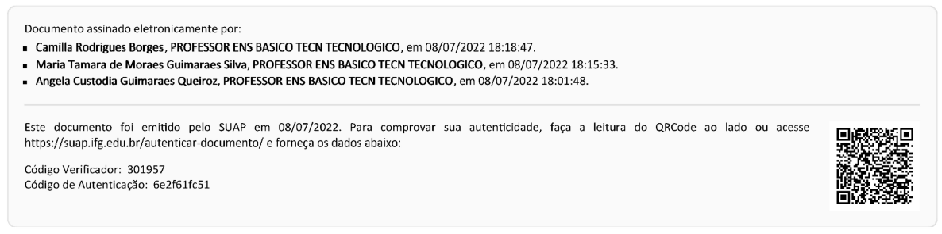
\includegraphics[width=0.79\textwidth]{./outros/fig/QR_CODE_V2.pdf}
    \end{tabular}
\end{center}
}
\end{atareuniao}
%---------------------------------------------------
\end{comment}
%---------------------------------------------------

% --------------------------------------------------
% Inserir folha de autorização para disponibilização
% --------------------------------------------------
%\linespread{0.87}\selectfont
%--------Cabe�alho do documento
\noindent\begin{minipage}[c][1.5cm][c]{3.5cm}

\includegraphics[width=1.5 \textwidth]{./outros/fig/IFGAnapolisHor2.png}
\end{minipage}\quad\quad\quad\qquad
\begin{minipage}{12cm}%10cm
\scriptsize\textbf{\ministerio}\\
\textbf{\secretaria}\\
\textbf{\instituto}\\
\textbf{\MakeTextUppercase{\campus}}\\
\textbf{\biblioteca}\\
\end{minipage}
%\vspace{-0.1cm}
\small{
\begin{center}
	\termo
\end{center}

\termodois

\noindent \textbf{Identifica\c{c}\~ao de Produ\c{c}\~ao T\'ecnico-Cient\'ifica}

\begin{tabular}{lllll}
\lbrack ~~\rbrack & Tese &  & \lbrack ~~\rbrack & Artigo Cient\'ifico \\ 
\lbrack ~~\rbrack & Disserta\c{c}\~ao &  & \lbrack ~~\rbrack & Cap\'itulo de Livro \\ 
\lbrack ~~\rbrack & Monografia -- Especializa\c{c}\~ao &  & \lbrack ~~\rbrack & Livro \\ 
\lbrack X\rbrack & TCC -- Gradua\c{c}\~ao &  & \lbrack ~~\rbrack & Trabalho Apresentado em Evento \\ 
\lbrack ~~\rbrack & Produto T\'ecnico e Educacional -- Tipo: & \multicolumn{3}{l}{\hrulefill} \\ 
\end{tabular}

\quad

\noindent Nome Completo do Autor:~\textbf{\alunonome~\alunosobre}

\noindent Matr\'icula:~\textbf{\matricula}

\noindent T\'ituto do Trabalho:~\textbf{\tituloprincipal}

\noindent \textbf{Autoriza\c{c}\~ao -- Marque uma das op\c{c}\~oes}

\begin{enumerate}
	\item (X) Autorizo disponibilizar meu trabalho no Reposit\'orio Digital do IFG (acesso aberto);
	\item (~) Autorizo disponibilizar meu trabalho no Reposit\'orio Digital do IFG somente ap\'os a data 20/10/20 (Embargo);
	\item (~) N\~ao autorizo disponibilizar meu trabalho no Reposit\'orio Digital do IFG (acesso restrito)
\end{enumerate}

\noindent Ao indicar a op\c{c}\~ao \textbf{2 ou 3}, marque a justificativa:
\begin{description}
	\item[(~~)] O documento est\'a sujeito a registro de patente.
	\item[(~~)] O documento pode vir a ser publicado como livro, cap\'itulo de livro ou artigo.
	\item[(~~)] Outra justificativa: \hrulefill
\end{description}

\begin{center}
	\textbf{\declaracao}
\end{center}

\noindent O(A) referido(a) autor(a) declara que:

\textbf{(i)}~o documento \'e seu trabalho original, det\'em os direitos autorais de produ\c{c}\~ao t\'ecnico-cient\'ifica e n\~ao infringe os direitos de qualquer outro pessoa ou entidade;

\textbf{(ii)}~\termotres

\textbf{(iii)}~cumpriu quaisquer obriga\c{c}\~oes exigidas por contrato ou acordo, caso o documento entregue seja baseado em trabalho finaciado ou apoiado por outra institui\c{c}\~ao que n\~ao o \entidade.

%\todaydia
\begin{flushright}
An\'apolis, {\diaata~de~\mesata}~de~{\todayano}
\end{flushright}

\begin{center}
\begin{tabular}{c}

\includegraphics[width=0.19 \textwidth]{./outros/fig/minhaAssinatura2.png} \\ 
\multicolumn{1}{c}{~\alunonome \alunosobre} \\ 
%\multicolumn{1}{c}{\hrulefill} \\ 
\end{tabular}
\end{center}
}%Fim \small

\linespread{1.3}\selectfont
%Retirando 
%\includepdf[pages={5}, fitpaper=true]{folhaTermo.pdf}.
%---------------------------------------------------
\begin{comment}% Descomente para aparecer O Termo de Autorização da biblioteca

\linespread{0.87}\selectfont
%--------Cabeçalho do documento
\noindent\begin{minipage}[c][1.5cm][c]{3.5cm}

\includegraphics[width=1.5 \textwidth]{./outros/fig/IFGAnapolisHor2.png}
\end{minipage}\quad\quad\quad\qquad
\begin{minipage}{12cm}%10cm
\scriptsize\textbf{\ministerio}\\
\textbf{\secretaria}\\
\textbf{\instituto}\\
\textbf{\MakeTextUppercase{\campus}}\\
\textbf{\biblioteca}\\
\end{minipage}
%\vspace{-0.1cm}
\small{
\begin{center}
	\termo
\end{center}

\termodois

\noindent \textbf{Identifica\c{c}\~ao de Produ\c{c}\~ao T\'ecnico-Cient\'ifica}

\begin{tabular}{lllll}
\lbrack ~~\rbrack & Tese &  & \lbrack ~~\rbrack & Artigo Cient\'ifico \\ 
\lbrack ~~\rbrack & Disserta\c{c}\~ao &  & \lbrack ~~\rbrack & Cap\'itulo de Livro \\ 
\lbrack ~~\rbrack & Monografia -- Especializa\c{c}\~ao &  & \lbrack ~~\rbrack & Livro \\ 
\lbrack X\rbrack & TCC -- Gradua\c{c}\~ao &  & \lbrack ~~\rbrack & Trabalho Apresentado em Evento \\ 
\lbrack ~~\rbrack & Produto T\'ecnico e Educacional -- Tipo: & \multicolumn{3}{l}{\hrulefill} \\ 
\end{tabular}

\quad

\noindent Nome Completo do Autor:~\textbf{\alunonome~\alunosobre}

\noindent Matr\'icula:~\textbf{\matricula}

\noindent T\'ituto do Trabalho:~\textbf{\tituloprincipal}

\noindent \textbf{Autoriza\c{c}\~ao -- Marque uma das op\c{c}\~oes}

\begin{enumerate}
	\item (X) Autorizo disponibilizar meu trabalho no Reposit\'orio Digital do IFG (acesso aberto);
	\item (~) Autorizo disponibilizar meu trabalho no Reposit\'orio Digital do IFG somente ap\'os a data 20/10/20 (Embargo);
	\item (~) N\~ao autorizo disponibilizar meu trabalho no Reposit\'orio Digital do IFG (acesso restrito)
\end{enumerate}

\noindent Ao indicar a op\c{c}\~ao \textbf{2 ou 3}, marque a justificativa:
\begin{description}
	\item[(~~)] O documento est\'a sujeito a registro de patente.
	\item[(~~)] O documento pode vir a ser publicado como livro, cap\'itulo de livro ou artigo.
	\item[(~~)] Outra justificativa: \hrulefill
\end{description}

\begin{center}
	\textbf{\declaracao}
\end{center}

\noindent O(A) referido(a) autor(a) declara que:

\textbf{(i)}~o documento \'e seu trabalho original, det\'em os direitos autorais de produ\c{c}\~ao t\'ecnico-cient\'ifica e n\~ao infringe os direitos de qualquer outro pessoa ou entidade;

\textbf{(ii)}~\termotres

\textbf{(iii)}~cumpriu quaisquer obriga\c{c}\~oes exigidas por contrato ou acordo, caso o documento entregue seja baseado em trabalho finaciado ou apoiado por outra institui\c{c}\~ao que n\~ao o \entidade.

%\todaydia
\begin{flushright}
An\'apolis, {\diaata~de~\mesata}~de~{\todayano}
\end{flushright}

\begin{center}
\begin{tabular}{c}

\includegraphics[width=0.19 \textwidth]{./outros/fig/minhaAssinatura2.png} \\ 
\multicolumn{1}{c}{~\alunonome \alunosobre} \\ 
%\multicolumn{1}{c}{\hrulefill} \\ 
\end{tabular}
\end{center}
}%Fim \small

\linespread{1.3}\selectfont

\end{comment}
%---------------------------------------------------


% ---
% Dedicatória
% ---
%\begin{dedicatoria}
%	\vspace*{\fill}
%	\noindent
%	\begin{adjustwidth*}{}{5.5cm}     
%		Este trabalho é dedicado aos meus colegas de %classe e aos meus queridos pais.
%	\end{adjustwidth*}
%\end{dedicatoria}
% ---

% ---
% Agradecimentos
% ---
%\begin{agradecimentos}
%	Inserir os agradecimentos aos colaboradores à %execução do trabalho. 
%\end{agradecimentos}
% ---

% ---
% Epígrafe
% ---
\begin{epigrafe}
    \null\vfill % Cria o ponto no topo e empurra o conteúdo para baixo
		\vspace{3cm}
    \begin{flushright}
        \textit{Se você for receptivo e humilde, a matemática o conduzirá pela mão. Repetidas vezes, quando estive perdido sem saber como prosseguir, bastou-me esperar até sentir que a matemática me guiava pela mão. Ela me conduziu por um caminho inesperado, um caminho onde novas perspectivas se abrem, um caminho que leva a um território novo, onde é possível estabelecer uma base de operações, a partir da qual se pode observar os arredores e planejar o progresso futuro.} \\
        \vspace{0.3cm}
        (Paul Dirac)
    \end{flushright}
    \vspace*{0.5cm} % Garante uma margem mínima do fim da folha (ajuste se quiser mais baixo)
\end{epigrafe}



% ---

% ---
% RESUMOS
% ---

% resumo em português
\setlength{\absparsep}{18pt} % ajusta o espaçamento dos parágrafos do resumo
\begin{resumo}
\SingleSpacing
%Os resultados revelam que não existe uma técnica universalmente superior: o RLM-\textit{subagging} apresentou melhor desempenho para Mn e Ni, o RLM-\textit{bagging} mostrou-se superior para Fe, enquanto a RLM clássica demonstrou desempenho superior para Mo e Cr. O comportamento diferenciado entre os analitos é atribuído à complexidade espectral de cada elemento: o Fe, por apresentar maior densidade de linhas espectrais com potencial de autoabsorção e sobreposições com outros elementos da matriz, beneficia-se da agregação de múltiplos modelos. Em contrapartida, Mn, Mo, Cr e Ni têm sua relação espectral-concentração suficientemente capturada pela RLM clássica ou pelo RLM-\textit{subagging}, sem ganho adicional com o RLM-\textit{bagging}. Todos os modelos apresentaram R$^2$ superior a 0,9815, evidenciando elevada capacidade preditiva. Quanto à eficiência computacional, o RLM-\textit{subagging} mostrou-se em média 3,0 vezes mais rápido que o RLM-\textit{bagging}, configurando-se como alternativa equilibrada entre precisão e eficiência em aplicações quimiométricas sujeitas a restrições temporais.

A calibração multivariada é essencial para determinar a composição elementar de aço-ligas a partir de dados espectrométricos. Este trabalho investigou, em caráter exploratório, a aplicação das técnicas de reamostragem \textit{bootstrap}, \textit{bagging} e \textit{subagging} incorporadas à Regressão Linear Múltipla (RLM) para a estimativa quantitativa dos elementos Manganês (Mn), Molibdênio (Mo), Cromo (Cr), Níquel (Ni) e Ferro (Fe). Paralelamente, conduziu-se a modernização de um sistema legado monolítico em Java \textit{Desktop} para uma aplicação \textit{Web} em Python e Streamlit, adotando arquitetura desacoplada em três módulos de responsabilidade única. A validação do sistema reescrito e a fidelidade a lógica matemática original foram asseguradas por uma suíte de 92 testes automatizados desenvolvida com \texttt{pytest}, englobando 21 testes unitários, 60 testes de caixa-preta baseados nos arquivos do sistema legado e 11 testes de carga e estresse com matrizes de alta dimensão. Os resultados experimentais demonstraram que a eficiência das técnicas de \textit{ensemble} varia conforme o analito: a RLM clássica obteve menor \textit{Root-Mean-Square Error of Prediction} (RMSEP) para o Molibdênio e o Cromo; o RLM-\textit{bagging} obteve menor erro para o Ferro; e o RLM-\textit{subagging} apresentou melhor desempenho para o Manganês e o Níquel (neste último, com desempenho numericamente equivalente ao da RLM clássica, com diferença de 0,25\% no (RMSEP). Em termos de eficiência computacional, o RLM-\textit{subagging} reduziu o tempo de processamento em relação ao RLM-\textit{bagging} em quatro dos cinco analitos. A suíte de testes confirmou a equivalência numérica estrita para os métodos determinísticos e a estabilidade da aplicação sob exigência computacional elevada, comprovando a viabilidade da modernização arquitetural sem perda de acurácia científica.

\textbf{Palavras-chave}: \palavrachaveum. \palavrachavedois. \palavrachavetres. \palavrachavequatro. \palavrachavecinco.
\end{resumo}

% resumo em inglês
\begin{resumo}[Abstract]
\SingleSpacing
\begin{otherlanguage*}{english}
%---------------------------------------------------
%The results reveal that no universally superior technique exists: RLM-\textit{subagging} achieved the best performance for Mn and Ni, RLM-\textit{bagging} proved superior for Fe, while classical MLR demonstrated superior performance for Mo and Cr. The differentiated behavior among analytes is attributed to the spectral complexity of each element: Fe, due to its higher density of spectral lines with self-absorption potential and overlaps with other matrix elements, benefits from the aggregation of multiple models. In contrast, Mn, Mo, Cr and Ni have their spectral-concentration relationship sufficiently captured by classical MLR or MLR-\textit{subagging}, with no additional gain from MLR-\textit{bagging}. All models presented R$^2$ values above 0.9815, evidencing high predictive capacity. Regarding computational efficiency, MLR-\textit{subagging} proved on average 3.0 times faster than MLR-\textit{bagging}, establishing itself as a balanced alternative between accuracy and efficiency in chemometric applications subject to time constraints.
%------------------------

Multivariate calibration is essential for determining the elemental composition of alloy steels from spectrometric data. This study explored the application of bootstrap resampling, bagging, and subagging techniques incorporated into Multiple Linear Regression (MLR) for the quantitative estimation of Manganese (Mn), Molybdenum (Mo), Chromium (Cr), Nickel (Ni), and Iron (Fe). Concurrently, a legacy monolithic Java Desktop system was modernized into a Python and Streamlit Web application, adopting a decoupled architecture structured into three single-responsibility modules. The validation of the rewritten system and its fidelity to the original algorithmic core were ensured by a suite of 92 automated tests developed with pytest, encompassing 21 unit tests, 60 black-box tests based on legacy system outputs, and 11 load and stress tests with high-dimensional matrices. Experimental results demonstrated that the efficiency of ensemble techniques varies depending on the analyte: classical MLR achieved a lower Root-Mean-Square Error of Prediction (RMSEP) for Molybdenum and Chromium; MLR-bagging yielded the lowest error for Iron; and MLR-subagging exhibited superior performance for Manganese and Nickel (in the latter, with performance numerically equivalent to classical MLR, showing a 0.25\% difference in RMSEP). In terms of computational efficiency, MLR-subagging reduced processing time compared to MLR-bagging across four of the five analytes. The test suite confirmed strict numerical equivalence for deterministic methods and application stability under high computational demand, proving the feasibility of architectural modernization without loss of scientific accuracy.%


%------------------------

\textbf{Keywords}: Resampling. Multivariate Calibration. Bagging. Subagging. Chemometrics.
\end{otherlanguage*}
\end{resumo}

%% resumo em francês 
%\begin{resumo}[Résumé]
% \begin{otherlanguage*}{french}
%    Il s'agit d'un résumé en français.
% 
%   \textbf{Mots-clés}: latex. abntex. publication de textes.
% \end{otherlanguage*}
%\end{resumo}
%
%% resumo em espanhol
%\begin{resumo}[Resumen]
% \begin{otherlanguage*}{spanish}
%   Este es el resumen en español.
%  
%   \textbf{Palabras clave}: latex. abntex. publicación de textos.
% \end{otherlanguage*}
%\end{resumo}
%% ---

{%hidelinks
	\hypersetup{hidelinks}
	% ---
	% inserir lista de ilustrações
	% ---
	\pdfbookmark[0]{\listfigurename}{lof}
	\listoffigures* %Retirado
	\cleardoublepage
	% ---
	
	% ---
	% inserir lista de quadros
	% ---
	\pdfbookmark[0]{\listofquadrosname}{loq}
	\listofquadros* %Retirado
	\cleardoublepage
	% ---
	
	% ---
	% inserir lista de tabelas
	% ---
	\pdfbookmark[0]{\listtablename}{lot}
	\listoftables* %Retirando
	\cleardoublepage
	% ---
	
	% ---
	% inserir lista de abreviaturas e siglas (devem ser declarados no preambulo)
	% ---

\imprimirlistadesiglas %Retirando
%\cleardoublepage
	% ---
	
	% ---
	% inserir lista de símbolos (devem ser declarados no preambulo)
	% ---
\imprimirlistadesimbolos %Retirando
%\cleardoublepage
	% ---
	
	% ---
	% inserir o sumario
	% ---
	\pdfbookmark[0]{\contentsname}{toc}
	\tableofcontents*
	\cleardoublepage
	
}%hidelinks
% ---
%Este include provoca erro de compilação
% ---

% ----------------------------------------------------------
% ELEMENTOS TEXTUAIS
% ----------------------------------------------------------
\textual

\setcounter{table}{0}% Este comando foi colocado para forçar a contagem das tabelas apartir de 1,2 e etc
% ---
% 1 - Introdução
% ---
\chapter{Introdução}
\label{cha:introducao}
\index{Introdução}

A calibração multivariada desempenha um papel fundamental em diversas áreas da análise química e industrial, permitindo a estimação de concentrações a partir de dados instrumentais multivariados. No contexto específico da análise de aço-ligas, a determinação precisa da composição elementar (Mn, Cr, Mo, Ni, Fe) é crucial para garantir a qualidade e as propriedades desejadas do material. No entanto, a complexidade dos dados multivariados provenientes de métodos instrumentais de análise exige o uso de técnicas de calibração multivariada para obter estimativas com erro de predição quantificável (RMSEP, MAE, R$^2$).

Este estudo investiga, em caráter exploratório, a aplicação de técnicas de reamostragem (\textit{bootstrap}), \textit{bagging} e \textit{subagging} na Regressão Linear Múltipla (RLM) para a calibração multivariada de amostras de aço-ligas. A pesquisa busca preencher a lacuna de conhecimento sobre a aplicação dessas técnicas de \textit{ensemble} nesse contexto específico, fornecendo subsídios empíricos exploratórios para a quimiometria e exemplificando a modernização de sistemas computacionais de apoio à análise de aço-ligas~\cite{SKOOG:1997,HARDLE:2007,TIMM:2002}.

Como otimizar a calibração multivariada de amostras de aço-ligas para obter previsões mais precisas dos elementos Mn, Cr, Mo, Ni e Fe, considerando a complexidade inerente à análise de dados multivariados, a necessidade de alta precisão e a exigência de uma arquitetura de \textit{software} modular e verificável por testes automatizados para sustentar essa análise?

Este estudo contribui em dois eixos: (a) a aplicação de \textit{bagging} e \textit{subagging} à calibração de aço-ligas; (b) a migração de um sistema legado verificada por testes automatizados. Essa estratégia evidencia, de forma reprodutível, como preservar a corretude de um núcleo algorítmico crítico durante a reescrita completa de uma arquitetura de \textit{software}.

A originalidade da pesquisa é dupla. No eixo quimiométrico, reside na aplicação de técnicas de \textit{bagging} e \textit{subagging}, ainda pouco exploradas na análise de aço-ligas.

No eixo de engenharia de \textit{software}, reside na condução de uma reescrita \textit{black-box} em três estágios (\textit{Desktop} Java, \textit{Web} Vaadin/Spring, Python/Streamlit), com arquitetura final desacoplada em três módulos de responsabilidade única e validação por 92 testes automatizados, que verificam a equivalência numérica do núcleo determinístico (RLM) e a consistência estatística dos métodos estocásticos entre o sistema legado e o sistema reescrito.

Dado o conjunto amostral reduzido — característica inerente à aquisição dos dados espectrométricos utilizados —, os resultados devem ser interpretados como evidências preliminares do comportamento dessas técnicas nesse domínio, e não como afirmações definitivas de superioridade geral de um método sobre outro.

Analisar e comparar o desempenho das técnicas de \textit{bagging} e \textit{subagging} aplicadas à Regressão Linear Múltipla (RLM) na calibração multivariada de dados de amostras de aço-ligas, investigando, em caráter exploratório, tanto o comportamento preditivo quanto a eficiência computacional de cada abordagem, a partir de uma arquitetura de \textit{software} desenvolvida de forma incremental e validada a cada etapa da migração.

Esta pesquisa tem como objetivos específicos:
\begin{description}
 \item[a)] Aplicar as técnicas de reamostragem \textit{bootstrap}, \textit{bagging} e \textit{subagging} na calibração de dados espectrométricos de amostras de aço-ligas, empregando a Regressão Linear Múltipla (RLM) como modelo base, visando a estruturação de um fluxo analítico reprodutível e padronizado~\cite{Canty2001,rathnayake2022}.

 \item[b)] Realizar uma comparação sistemática entre os algoritmos RLM clássica, RLM-\textit{bagging} e RLM-\textit{subagging}, por meio da avaliação criteriosa da acurácia preditiva e da eficiência computacional de cada abordagem na análise quantitativa dos elementos Mn, Cr, Mo, Ni e Fe.

 \item[c)] Reaproveitar, em Java (JavaSE-17), o sistema \textit{Desktop} de calibração multivariada com RLM-\textit{bagging} e RLM-\textit{subagging} — desenvolvido na disciplina de Programação Orientada a Objetos, com arquitetura monolítica (em um único arquivo), biblioteca \gls{EJML}\footnote{A biblioteca \textit{Efficient Java Matrix Library} (EJML) é uma biblioteca de álgebra linear de alto desempenho para Java, projetada para manipulação eficiente de matrizes densas e esparsas.} e interface gráfica Swing/AWT —, refinando suas estruturas de dados e tratando inconsistências nas métricas de avaliação do algoritmo para servir como referência de validação e base de código legada.

 \item[d)] Desenvolver e disponibilizar um protótipo \textit{Web} reescrito em Python 3.12 e Streamlit, adotando arquitetura modular desacoplada em três módulos de responsabilidade única (\texttt{app.py}, \texttt{components.py} e \texttt{models.py}), que automatize o fluxo analítico de calibração multivariada por RLM, RLM-\textit{bagging} e RLM-\textit{subagging}, permitindo o carregamento de matrizes de calibração e teste, a configuração de hiperparâmetros, a execução de validação cruzada 5-\textit{fold} por \textit{grid search} e a geração automática de relatórios com métricas preditivas (RMSEP, MAE, R$^2$) e gráficos interativos Plotly.

 \item[e)] Garantir a equivalência comportamental e a qualidade do \textit{software} reescrito por meio da especificação de requisitos formais e da implementação de uma suíte de 92 testes automatizados com \texttt{pytest}, abrangendo testes unitários, testes de caixa-preta baseados em saídas do sistema legado e testes de estresse com matrizes sintetizadas de alta dimensão.
\end{description}

Esse protocolo funciona como validador de equivalência entre o sistema legado e o sistema reescrito em dois níveis: equivalência numérica estrita para a RLM determinística e consistência estatística, dentro de tolerâncias explícitas, para o \textit{bagging} e o \textit{subagging}, cujas sequências pseudoaleatórias diferem entre as duas linguagens.

Este trabalho está organizado da seguinte forma. A Seção~\ref{cha:tecboot} apresenta a revisão da literatura sobre a Regressão Linear Múltipla (RLM), a técnica de reamostragem \textit{bootstrap} e os conceitos de distribuição empírica e princípio \textit{plug-in}, essenciais à compreensão das abordagens investigadas. A Seção~\ref{sec:teclarea} descreve as técnicas de \textit{bagging} e \textit{subagging}, incluindo fundamentos teóricos e algoritmos.
% ---

% ---
% 2 - Seção 2(Desenvolvimento)
% ---
%------------------------------------------
\chapter{Revisão da literatura}\label{cap:desenvolvimento}
\label{cha:tecboot}
% -----------------------------------------
Esta seção apresenta a Regressão Linear Múltipla (RLM) e a técnica \textit{bootstrap}. Adicionalmente, são abordados conceitos como a teoria da probabilidade, distribuição empírica, princípio \textit{plug-in} e técnicas clássicas de reamostragem, fundamentais para a compreensão.
\begin{comment}
%-------------------------------------------------------
\section{Regressão Linear Múltipla}
%-------------------------------------------------------
A RLM é empregada quando é necessário estabelecer uma relação envolvendo mais de uma variável independente (\textit{\gls{x2}})
\begin{equation}
    \gls{y} = x_1b_1 + x_2b_2 +\ldots+ x_nb_n
\end{equation}
\begin{equation}
    b_j \in \gls{R}, \quad j = 1,2,\ldots,n
\end{equation}
ou, na forma matricial,
\begin{equation}
    y = [x_1 \quad x_2 \quad \ldots \quad \gls{x_n}]\left[\begin{array}{c}
b_1\\b_2\\\vdots \\b_n
\end{array}\right] \triangleq \textbf{xb}
\end{equation}

O procedimento de estimação é denominado regressão linear múltipla~\cite{KRAMER:1998,MARTENS:1989,Filzmoser2021,Schielzeth2020,revelas2024,paleologo2020,Dar2024,rathnayake2022}. Dispondo de dados de calibração
\begin{equation}
    \{(x^i,\gls{y^i}), \quad i = 1,2,\ldots,M \}
\end{equation}
ou, na forma matricial
\begin{equation}
X_{cal} =
\left[\begin{array}{c}
x^1\\x^2\\\vdots \\x^M
\end{array}\right]
\quad y_{cal} =
\left[\begin{array}{c}
y^1\\y^2\\\vdots \\y^M
\end{array}\right]
\end{equation}
onde a melhor estimativa no sentido de mínimos quadrados para o vetor de coeficientes \textbf{b} é dada pela pseudo-inversa de Moore-Penrose~\cite{DRAPER:1998,TIMM:2002}:
\begin{equation}
    \widehat{\textbf{b}} = \gls{X_cal^+} \textbf{y}_{cal}\triangleq (\textbf{X}_{cal}^{\textbf{T}} \textbf{X}_{cal})^{-1} \textbf{X}_{cal}^{\textbf{T}} \textbf{y}_{cal}
\end{equation}

Segundo Alin e Serneels~\cite{Alin2017} e Filzmoser e Nordhausen~\cite{Filzmoser2013}, métodos robustos se tornam necessários quando há violação das premissas da regressão linear múltipla.


As premissas de normalidade dos resíduos devem ser verificadas em modelos de calibração. Testes robustos de normalidade, especialmente apropriados para dados quimiométricos - que frequentemente apresentam estruturas complexas - são discutidos em estudos anteriores~\cite{Alin2017,Filzmoser2013}.
\end{comment}


\section{Regressão Linear Múltipla}

A RLM é uma técnica estatística empregada para modelar a relação linear entre uma variável dependente (resposta) ($\gls{y}$) e duas ou mais variáveis independentes (preditoras) ($\mathbf{X}$). O modelo, que inclui um termo de intercepto ($\beta_0$) e um termo de erro ($\varepsilon$), é formalizado como:
\begin{equation}
    \label{eq:rlm-modelo}
    \gls{y} = \beta_0 + x_1\beta_1 + x_2\beta_2 +\ldots+ x_n\beta_n + \varepsilon
\end{equation}
onde $\beta_j \in \mathbb{R}$ representa o coeficiente angular de cada preditor $x_j$, para $j = 1,2,\ldots,n$.

Dispondo de um conjunto de $M$ dados de calibração $\{(x^i,\gls{y^i}), \quad i = 1,2,\ldots,M \}$, o modelo pode ser expresso na forma matricial:
\begin{equation}
    \mathbf{y} = \mathbf{X}\mathbf{\beta} + \mathbf{\varepsilon}
\end{equation}
onde o vetor de resposta $\mathbf{y}$ e a matriz de calibração $\mathbf{X}$ (incluindo a coluna de uns para o intercepto) são definidos por:
\begin{equation}
    \mathbf{X} =
    \left[\begin{array}{ccccc}
    1 & x_{1}^1 & x_{2}^1 & \ldots & x_{n}^1 \\
    1 & x_{1}^2 & x_{2}^2 & \ldots & x_{n}^2 \\
    \vdots & \vdots & \vdots & \ddots & \vdots \\
    1 & x_{1}^M & x_{2}^M & \ldots & x_{n}^M
    \end{array}\right]
    \quad \mathbf{y} =
    \left[\begin{array}{c}
    y^1\\y^2\\\vdots \\y^M
    \end{array}\right]
\end{equation}
O vetor de coeficientes populacionais é $\mathbf{\beta} = [\beta_0, \beta_1, \ldots, \beta_n]^{\textbf{T}}$.

\subsection{Estimação dos Coeficientes}
O procedimento de estimação é conhecido como \gls{MQO}. O MQO busca o vetor de coeficientes estimados $\widehat{\mathbf{\beta}}$ que minimiza a \gls{SQR}.

A melhor estimativa $\widehat{\mathbf{\beta}}$ no sentido de mínimos quadrados é dada pela solução da pseudo-inversa de Moore-Penrose \cite{DRAPER:1998,TIMM:2002}:
\begin{equation}
    \label{eq:rlm-pseudo}
    \widehat{\mathbf{\beta}} = \mathbf{X}^+ \mathbf{y} \triangleq (\mathbf{X}^{\textbf{T}} \mathbf{X})^{-1} \mathbf{X}^{\textbf{T}} \mathbf{y}
\end{equation}
onde $\mathbf{X}^{+}$ é a pseudo-inversa da matriz $\mathbf{X}$.


\subsection{Premissas e Métodos Robustos}
A validade das estimativas obtidas pelo MQO depende do cumprimento das premissas clássicas da regressão linear. Em dados espectrais, a colinearidade entre variáveis e a presença de outliers violam com frequência esses pressupostos~\cite{Alin2017,Filzmoser2013}.

Métodos robustos tornam-se indispensáveis quando há violação das premissas da regressão linear múltipla, especialmente na presença de \textit{outliers} \cite{Alin2017,Filzmoser2013}. A verificação da normalidade dos resíduos, em particular, é crucial e discutida em detalhes em estudos anteriores \cite{Alin2017,Filzmoser2013}.


% ----------------------------------------------------
\section{A Técnica de \textit{Bootstrap}}
% ----------------------------------------------------
%A inferência estatística estabelece propriedades para a população \textbf{X} a partir da análise de uma amostra aleatória dessa população~\cite{DRAPER:1998,JOHNSON:2001,CHATTERJEE:2006}. O método \textit{bootstrap} é um procedimento computacional que fornece a medida do nível de precisão da inferência estatística, como por exemplo, média, desvio padrão e erro padrão~\cite{yeon2023,alfons2022,wan2023,du2024,jensen2024}. A ideia básica do \textit{bootstrap} é inferir estatisticamente as propriedades de interesse a partir da análise de amostras aleatórias extraídas da população original sem a necessidade de conhecer a distribuição de dados a priori, o que constitui significativa vantagem sobre outras técnicas~\cite{HARDLE:2007,TIMM:2002}.

A inferência estatística estabelece propriedades para a população \textbf{X} a partir da análise
de uma amostra aleatória dessa população~\cite{DRAPER:1998,JOHNSON:2001,CHATTERJEE:2006}. O método \textit{bootstrap} é um procedimento computacional que fornece a medida do nível de precisão da inferência estatística, como por exemplo, média, desvio padrão e erro padrão~\cite{yeon2023,alfons2022,wan2023,du2024,jensen2024}.

A ideia básica do \textit{bootstrap} é inferir estatisticamente as propriedades de interesse a partir da análise de amostras aleatórias extraídas da população original sem a necessidade de conhecer a distribuição de dados a priori, o que dispensa a suposição prévia de uma distribuição paramétrica dos dados~\cite{HARDLE:2007,TIMM:2002}.

Quando o parâmetro populacional de interesse é desconhecido, procura-se estimá-lo por
reamostragem aleatória. Inicialmente, considera-se a \textbf{população} 
$\mathbf{x} = [x_1, x_2, \ldots, x_N]$. A partir dela, seleciona-se uma 
\textbf{amostra} $\mathbf{X} = [x_1, x_2, \ldots, x_n]$, formada por $n$ elementos 
independentes retirados da população. 

%Para avaliar a variabilidade das estimativas, aplica-se o método de \textbf{\textit{bootstrap}}, que consiste em gerar $m$ \textbf{reamostras} $\mathbf{X}^{*1}, \mathbf{X}^{*2}, \ldots, \mathbf{X}^{*m}$, obtidas por sorteio com reposição a partir da amostra original. Formalmente, cada reamostra é definida como \[ \mathbf{X}^{*i} \sim \text{\textit{Bootstrap}}(\mathbf{X}), \quad i = 1,2,\ldots,m,\] onde $\text{\textit{Bootstrap}}(\mathbf{X})$ denota a distribuição empírica gerada pela amostra. Em seguida, calcula-se uma estatística $s(\mathbf{X}^{*i})$ para cada reamostra, gerando uma distribuição empírica das estimativas. Esse processo é ilustrado na Figura~\ref{fig:bootstrap}.

Para avaliar a variabilidade das estimativas, aplica-se o método de \textbf{\textit{bootstrap}}, que consiste em gerar $m$ \textbf{reamostras} 
$\mathbf{X}^{*1}, \mathbf{X}^{*2}, \ldots, \mathbf{X}^{*m}$, obtidas por sorteio com reposição a partir da amostra original. Formalmente, cada reamostra é definida como
\[
\mathbf{X}^{*i} \sim \text{\textit{Bootstrap}}(\mathbf{X}), \quad i = 1,2,\ldots,m,
\]
onde $\text{\textit{Bootstrap}}(\mathbf{X})$ denota a distribuição empírica gerada pela amostra.

Em seguida, calcula-se uma estatística $s(\mathbf{X}^{*i})$ para cada reamostra, 
gerando uma distribuição empírica das estimativas. Esse processo é ilustrado 
na Figura~\ref{fig:bootstrap}.

\begin{figure}[H]
    \centering
		\caption{Exemplo do método \textit{bootstrap}.}
		\resizebox{0.70\textwidth}{!}{
    \begin{tikzpicture}[
        box/.style={rectangle, draw, minimum width=2.5cm, minimum height=1cm, align=center},
        arrow/.style={-Stealth, thick}
    ]
    
    % Nodo População
    \node[box] (Pop) at (0,2) {$\mathbf{x} = [x_1, x_2, \dots, x_N]$ \\ População};
    
    % Nodo Amostra
    \node[box] (X) at (0,0) {$\mathbf{X} = [x_1, x_2, \dots, x_n]$ \\ Amostra};
    
    % Nodos de Reamostras
    \node[box] (X1) at (-3,-2) {$\mathbf{X}^{*1}$};
    \node[box] (X2) at (0,-2) {$\mathbf{X}^{*2}$};
    \node[box, dotted] (dots) at (3,-2) {$\dots$};
    \node[box] (Xm) at (6,-2) {$\mathbf{X}^{*m}$};
    
    % Nodos de Estatísticas
    \node[box] (sX1) at (-3,-4) {$s(\mathbf{X}^{*1})$};
    \node[box] (sX2) at (0,-4) {$s(\mathbf{X}^{*2})$};
    \node[box, dotted] (sdots) at (3,-4) {$\dots$};
    \node[box] (sXm) at (6,-4) {$s(\mathbf{X}^{*m})$};
    
    % Setas População -> Amostra
    \draw[arrow] (Pop) -- (X) node[midway, right] {Amostragem};
    
    % Setas Amostra -> Reamostras
    \draw[arrow] (X) -- (X1) node[midway, above left] {Reamostras};
    \draw[arrow] (X) -- (X2);
    \draw[arrow] (X) -- (dots);
    \draw[arrow] (X) -- (Xm) node[midway, above right] {Reamostras};
    
    % Setas Reamostras -> Estatísticas
    \draw[arrow] (X1) -- (sX1) node[midway, left] {Estatísticas};
    \draw[arrow] (X2) -- (sX2);
    \draw[arrow] (dots) -- (sdots);
    \draw[arrow] (Xm) -- (sXm) node[midway, right] {Estatísticas};
    
    \end{tikzpicture}
		}
\label{fig:bootstrap}
\legend{\footnotesize Fonte:~\oautor}
\end{figure}

%A Figura~\ref{fig:bootstrap} ilustra o procedimento de \textit{bootstrap} em quatro etapas. O primeiro passo (primeiro retângulo) representa a população completa, denotada por $\mathbf{x} = [x_1, x_2, \dots, x_N]$, da qual é extraída uma amostra através do processo de amostragem. O segundo passo (segundo retângulo) corresponde ao conjunto de dados observados, denotado por $\mathbf{X} = [x_1, x_2, \dots, x_n]$. O terceiro passo (terceiro conjunto de retângulos) corresponde à extração de amostras \textit{bootstrap}, obtidas por reamostragem com reposição a partir de $\mathbf{X}$. O quarto passo (quarto conjunto de retângulos) mostra as replicações \textit{bootstrap}, nas quais uma função estatística $s(\gls{gamma})$ é recalculada $m$ vezes, sendo $m$ o número total de replicações.

A Figura~\ref{fig:bootstrap} ilustra o procedimento de \textit{bootstrap} em quatro etapas. O primeiro passo (primeiro retângulo) representa a população completa, denotada por $\mathbf{x} = [x_1, x_2, \dots, x_N]$, da qual é extraída uma amostra através do processo de amostragem. O segundo passo (segundo retângulo) corresponde ao conjunto de dados observados, denotado por $\mathbf{X} = [x_1, x_2, \dots, x_n]$.

O terceiro passo (terceiro conjunto de retângulos) corresponde à extração de amostras \textit{bootstrap}, obtidas por reamostragem com reposição a partir de $\mathbf{X}$. O quarto passo (quarto conjunto de retângulos) mostra as replicações \textit{bootstrap}, nas quais uma função estatística $s(\gls{gamma})$ é recalculada $m$ vezes, sendo $m$ o número total de replicações.

Nas seções subsequentes, são discutidos conceitos fundamentais relacionados a amostras aleatórias e probabilísticas, bem como a distribuição empírica e o princípio \textit{plug-in}. A apresentação desses tópicos tem como objetivo fornecer a base teórica necessária para a compreensão dos procedimentos de inferência estatística realizados a partir de amostras \textit{bootstrap}.

%------------------------------------------------
\subsection{\textit{Bootstrap}}
\label{sec:boot}
\index{A Técnica de \textit{Bootstrap}!\textit{Bootstrap}}
%-----------------------------------------------
Uma amostra aleatória $\gls{x_al} = [x_{al1},\ldots, x_{aln}]$ é extraída da distribuição de probabilidade \textbf{D}. O parâmetro de interesse $\theta = \gls{t(d)}$ é desconhecido e será estimado com base na amostra observada $\gls{x_al}$, resultando no estimador $\widehat{\theta} = t(\gls{x_al})$.

%-----------------------------------------------
\subsection{Estimativa \textit{Bootstrap}}
\label{sec:estboot}
\index{A Técnica de \textit{Bootstrap}!Estimativa \textit{Bootstrap}}
%-----------------------------------------------
O método \textit{bootstrap} necessita inicialmente das amostras \textit{bootstrap} para depois aplicar as replicações \textit{bootstrap}, como foi visto na Figura~\ref{fig:bootstrap}. Suponha a distribuição empírica $\widehat{\textbf{d}}$, com probabilidade $\frac{1}{n}$ em cada valor de $x_i$, tendo $i = 1, 2,\ldots, n$. A amostra \textit{bootstrap} é definida como sendo a amostra aleatória de tamanho $n$ extraída de $\widehat{\textbf{d}}$, representada por $\gls{x^*} =[x_1^*, x_2^*,\ldots, x_n^*]$~\cite{EFRON:1994}. As amostras \textit{bootstrap} são obtidas por reamostragem com reposição, podendo haver repetições dos elementos da amostra original $[x_1, x_2,\ldots, x_n]$.

As replicações \textit{bootstrap} são representadas por
\begin{equation}
    \widehat{\theta} = s(\gls{x^*}),
\end{equation}
onde $s(\gls{gamma})$ é a função estatística a ser aplicada sobre as amostras \textit{bootstrap}. Por exemplo, se $s(x)$ for a média amostral $\overline{x}$, então $s(\gls{x^*})$ é a média da amostra \textit{bootstrap}
\begin{equation}
    \overline{x^*} = \frac{1}{n} \sum_{i=1}^{n} x_i^*.
\end{equation}

\medskip
%--------------------------------------------------
\begin{minipage}{0.80\textwidth}
\begin{algorithm2e}[H]
 \dontprintsemicolon %\dontprintsemicolon
 \linesnumbered%\linesnumbered
 %%\nocaptionofalgo
 \SetLine
 \BlankLine
 \Entrada{Amostra original $x = (x_1, x_2, \ldots, x_n)$, estatística de interesse $\theta = s(x)$, número de replicações \textit{bootstrap} $m$}
 \Saida{Estimativa \textit{bootstrap} \gls{hat_theta^*}, erro padrão \textit{bootstrap}, intervalo de confiança \textit{bootstrap}}
 \BlankLine
\Inicio{
  Selecione a quantidade de amostras independentes ~$m$,~\{$x^{*1},x^{*2},\ldots,x^{*m}$\}, tendo tamanho
 $m$ e podendo haver repetições de  $x$.\;
Avaliar a replicação \textit{bootstrap} para amostra \textit{bootstrap}, $\widehat{\theta}^*(b)= s(x^{*b})$ $\quad$ $b = 1,2,\ldots ,m$. \;}
\caption{Estimativa das replicações \textit{bootstrap}. \label{alg:bootstrap}}
\end{algorithm2e}
\legend{\footnotesize Fonte:~\oautor}
\end{minipage}

O Algoritmo~\ref{alg:bootstrap} \cite{EFRON:1993} mostra a descrição do procedimento para
utilizar a estimativa \textit{bootstrap}, replicando o estimador $\widehat{\theta} = s(x)$ a partir dos dados $x$ observados.

%-------------------------------------------------
\subsection{O Número de Replicações \textit{Bootstrap} \textit{m}}
\label{sec:numreplboot}
\index{A Técnica de \textit{Bootstrap}!O Número de Replicações \textit{Bootstrap} $m$}
%-------------------------------------------------
A estimativa \textit{bootstrap} ideal é obtida através de uma boa escolha do número de replicações
$\gls{m} = \infty$, com o $\gls{hat_se}_{\infty}$ igual à estimativa \textit{plug-in} $se_{\widehat{\textbf{d}}}(\widehat{\theta}^*)$~\cite{EFRON:1993}.
O número de replicações \textit{bootstrap} influencia diretamente o tempo computacional
gasto ao processar as replicações, principalmente se a função $s(x)$ do estimador $\widehat{\theta} = s(x)$ for muito
complexa. Portanto, se não for possível obter infinitas replicações, deve-se utilizar o maior número possível de replicações.

%---------------------------------------------------------------------------------------------------------

%É necessário que estimadores apresentem bom comportamento: baixo erro de predição e pequeno desvio padrão. A estimativa \textit{bootstrap} para o erro padrão geralmente apresenta erro de predição relativamente pequeno. A estimativa \textit{bootstrap} ideal $\widehat{se}_{\infty}$ possui baixa variabilidade entre estimativas com erro de predição quase nulo de $se_{\widehat{\textbf{d}}}(\widehat{\theta^*})$, pelo menos em um sentido assintótico. Esta propriedade decorre do fato de que $\widehat{se}_m$ é a estimativa \textit{plug-in} de $se_{\widehat{\textbf{d}}}(\widehat{\theta^*})$. Não é difícil mostrar que $\widehat{se}_m$ sempre possui desvio padrão maior que $\widehat{se}_{\infty}$~\cite{EFRON:1993}. A questão que se coloca é: \textbf{o quanto maior}?

É necessário que estimadores apresentem bom comportamento: baixo erro de predição e pequeno desvio padrão. A estimativa \textit{bootstrap} para o erro padrão geralmente apresenta erro de predição relativamente pequeno. A estimativa \textit{bootstrap} ideal $\widehat{se}_{\infty}$ possui baixa variabilidade entre estimativas com erro de predição quase nulo de $se_{\widehat{\textbf{d}}}(\widehat{\theta^*})$, pelo menos em um sentido assintótico.

Esta propriedade decorre do fato de que $\widehat{se}_m$ é a estimativa \textit{plug-in} de $se_{\widehat{\textbf{d}}}(\widehat{\theta^*})$. Não é difícil mostrar que $\widehat{se}_m$ sempre possui desvio padrão maior que $\widehat{se}_{\infty}$~\cite{EFRON:1993}. A questão que se coloca é: \textbf{o quanto maior}?

%--------------------------------------------------------------------------------------------------

Uma resposta aproximada, porém satisfatória, pode ser encontrada utilizando o coeficiente de variação de $\widehat{se}_{m}$ em relação à sua expectativa. O aumento da variabilidade decorrente da interrupção do processo após $m$ replicações \textit{bootstrap}, em vez de permitir que $m$ tenda ao infinito, resulta em um aumento do coeficiente de variação:
\begin{equation}
    cv(\widehat{se}_{m}) = \sqrt{[cv(\widehat{se}_\infty)]^2 + \frac{E(\Delta) + 2}{4m}}.
\label{eq:2.19}
\end{equation}

O parâmetro \gls{Delta} mede o tamanho da distribuição de $\widehat{\theta}^*$: $\Delta$ é zero para a distribuição normal; na prática, $\Delta$ geralmente é maior que 10. O coeficiente de variação na Equação~(\ref{eq:2.19}) incorpora tanto a variabilidade devida à reamostragem \textit{bootstrap} quanto a variabilidade devida à amostragem da população original.


A estimativa ideal $\widehat{se}_\infty = se_{\widehat{\mathbf{d}}}(\widehat{\theta}^*)$ não é perfeita~\cite{EFRON:1993}. Pode haver variabilidade estatisticamente significativa na estimativa $se_{\mathbf{d}}(\widehat{\theta})$ devido à variabilidade de $\widehat{\mathbf{d}}$ em relação a $\mathbf{d}$. Por exemplo, se $\{x_1, x_2, \ldots, x_n\}$ for uma amostra aleatória de uma distribuição normal e $\widehat{\theta} = \overline{x}$, então $cv(\widehat{se}_\infty) = \frac{1}{\sqrt{2n}}$, resultando em $0,22$ para $n = 10$.

A Equação~(\ref{eq:2.19}) tem uma consequência prática importante: dados os valores típicos de $cv(\widehat{se}_\infty)$ e $\Delta$ encontrados na prática, $cv(\widehat{se}_m)$ não será muito maior que $cv(\widehat{se}_\infty)$ quando $m \geq 200$.

%-----------------------------------------------------------------------------------
\begin{table}[!htbp]
\centering
\begin{threeparttable}
\caption{O coeficiente de variação.}
\begin{tabular}{lllllll}
\hline
 &  &  m\tnote{a} $\to$ &  &  &  &  \\ 
 &  & 25 & 50 & 100 & 200 & $\infty$ \\ 
\hline
 $cv(\widehat{se}_{\infty})$\tnote{b} & 0,25 & 0,29 & 0,27 & 0,26 & 0,25 & 0,25 \\ 
\multicolumn{1}{c}{$\downarrow$} & 0,20 & 0,24 & 0,22 & 0,21 & 0,21 & 0,20 \\ 
 & 0,15 & 0,21 & 0,18 & 0,17 & 0,16 & 0,15 \\ 
 & 0,10 & 0,17 & 0,14 & 0,12 & 0,11 & 0,10 \\ 
 & 0,05 & 0,15 & 0,11 & 0,09 & 0,07 & 0,05 \\ 
 & 0,00 & 0,14 & 0,10 & 0,07 & 0,05 & 0,00 \\ 
\hline
\end{tabular}
\begin{tablenotes}[flushleft] % Garante o alinhamento exatamente abaixo do analito
    \footnotesize
    \item Fonte:~EFRON, B.; TIBSHIRANI, R. J. \textit{An Introduction to the Bootstrap}, USA: Chapman \& Hall/CRC, 1993, p.53.
	\item[a] Número de amostras \textit{bootstrap}.
	\item[b] Coeficiente de variação.
\end{tablenotes}
\label{tab:coefvaria}
\end{threeparttable}
\end{table}
%-----------------------------------------------------------------------------------

A Tabela~\ref{tab:coefvaria} compara $cv(\widehat{se}_m)$ com $cv(\widehat{se}_{\infty})$ para várias escolhas de $m$, assumindo $\Delta = 0$. Para $cv(\widehat{se}_\infty)\geq 0{,}10$, com $m=100$ o $cv(\widehat{se}_m)$ excede o ideal em no máximo \num{0,02} (Tabela~\ref{tab:coefvaria}). Efron~\cite{EFRON:1993} sugere duas regras práticas através da sua experiência:

\begin{enumerate}[label=\alph*)]
    \item Mesmo um número pequeno de replicações \textit{bootstrap}, como $m = 25$, é geralmente informativo; $m = 50$ é frequentemente suficiente para uma boa estimativa de $se_{\mathbf{d}}(\widehat{\theta})$.
    \item Segundo Efron e Tibshirani~\cite{EFRON:1993}, raramente são necessárias mais de 200 replicações para o erro padrão; para intervalos de confiança.
\end{enumerate}

A Tabela~\ref{tab:coefvaria} mostra a variação de $\widehat{se}_m$ em função do coeficiente de variação da estimativa ideal $\widehat{se}_{\infty}$ e do número de amostras \textit{bootstrap} $m$, obtidos da Equação~(\ref{eq:2.19}) assumindo $\Delta = 0$.
%-----------------------------------------------------------------------------------

\section{Reamostragem Aleatória}

O processo de reamostragem é realizado a partir da seleção aleatória de números inteiros $\{j_1, j_2, \ldots, j_n\}$, cada um com probabilidade $1/n$. Uma amostra aleatória de tamanho $n$ é definida pela seleção aleatória de $n$ unidades $\{u_1, u_2, \ldots, u_n\}$ extraídas da população \gls{u} (ver Figura~\ref{fig:amoale}), onde \gls{u} é a população de números inteiros selecionados para gerar variáveis aleatórias. 

A população \gls{v} é formada pelos valores selecionados de \gls{u} de acordo com os valores de $j$, sendo constituída por $\{v_1, v_2, \ldots, v_n\}$. Esta população é criada por um dispositivo (como um software) responsável por gerar as amostras aleatórias. Por meio dos valores $\{j_1, j_2, \ldots, j_n\}$ selecionados, pode-se determinar quais membros de \gls{v} serão escolhidos para a amostra aleatória:
\begin{equation*}
    u_1 = v_{j_1}, \quad u_2 = v_{j_2}, \quad \ldots, \quad u_n = v_{j_n}.
\end{equation*}

Sendo \gls{x_i} uma medida da unidade $u_i$ para $i = 1, 2, \ldots, n$, o conjunto de dados observados será
\begin{equation}
    \gls{x} = \{x_1, x_2, \ldots, x_n\}.
\end{equation}
%----------------------------------------------------------------------
\begin{figure}[H]%ht!
\centering
\caption{Processo de amostragem aleatória.}
\resizebox{0.25\textwidth}{!}{
\begin{tikzpicture}[
    box/.style={rectangle, draw, minimum height=1.5cm, text width=4cm, align=center},
    arrow_style/.style={-Stealth, thick},
    label_style/.style={font=\small, align=center}
]
% Nodos principais
\node[box] (populacao_v) at (0, 0) {\textbf{População $\mathbf{v}$}\\ $v_1, v_2, \ldots, v_n$};
\node[box, below=1.5cm of populacao_v] (amostra_u) {\textbf{Amostra $\mathbf{u}$}\\ $u_1, u_2, \ldots, u_n$};
\node[box, below=1.5cm of amostra_u] (medidas) {\textbf{Medidas $\mathbf{x}$}\\ $x_1, x_2, \ldots, x_n$};

% Setas e rótulos
\draw[arrow_style] (populacao_v.south) -- node[right, label_style] {Seleção por índices\\ $j_1, j_2, \ldots, j_n$\\ $u_i = v_{j_i}$} (amostra_u.north);
\draw[arrow_style] (amostra_u.south) -- node[right, label_style] {Observação\\ $x_i = $ medida de $u_i$} (medidas.north);

\end{tikzpicture}
}
\legend{\footnotesize Fonte:~\oautor}
\label{fig:amoale}
\end{figure}
%----------------------------------------------------------------------
Se as unidades da amostra $\{u_1, u_2, \ldots, u_n\}$ são observadas, obtêm-se as medidas correspondentes $\{x_1, x_2, \ldots, x_n\}$, que formam o vetor de dados \gls{x}.
%----------------------------------------------------------------------

%----------------------------------------------------------------------
\section{Teoria da Probabilidade}
\label{sec:teopro}
%----------------------------------------------------------------------
A partir de uma amostra aleatória \gls{x_al}, deve-se inferir a distribuição de probabilidade da população completa $\mathbf{X} = [X_1, X_2, \ldots, X_n]$, onde $X_i$ representa a variável aleatória associada à $i$-ésima observação. A teoria da probabilidade segue o raciocínio oposto: a partir do conhecimento da distribuição de probabilidade da população $\mathbf{X}$, deduzem-se as propriedades das amostras aleatórias e das estatísticas calculadas a partir delas.

Seja \gls{x_al2} o resultado da rolagem de um dado não viciado. Por exemplo, no lançamento de um dado cúbico de 6 faces, onde todas as faces possuem probabilidades iguais de ocorrência, obtém-se como resultado 1, 2, 3, 4, 5 ou 6. Em notação probabilística, tem-se
\begin{equation}
    \Pr\{x_{al} = k\} = \frac{1}{6}, \quad \text{para } k = 1, 2, 3, 4, 5, 6.
\end{equation}

%------------------------------------------------------------------------------------------
A quantidade aleatória que possua a probabilidade de ser selecionada como \gls{x_al2} é chamada de \textit{variável aleatória}. Na teoria da probabilidade, a notação utilizada para definir a frequência \gls{f_k} é dada por
\begin{equation}
    f_k = \Pr\{x_{al} = k\}.
\end{equation}

Na rolagem do dado não viciado, tem-se $f_k = \frac{1}{6}$ para $k = 1, 2, \ldots, 6$. A distribuição de probabilidade para a variável aleatória $x_{al}$ será denotada por \gls{f}. Aqui, \gls{f} é o vetor de frequências
\begin{equation}
    \mathbf{f} = (f_1, f_2, \ldots, f_6) = \left(\frac{1}{6}, \frac{1}{6}, \ldots, \frac{1}{6}\right).
\end{equation}

Podem-se encontrar também amostras com variáveis aleatórias \gls{x_al2} na forma da distribuição binomial de tamanho $n$ e probabilidade de sucesso $p$, denotada
\begin{equation}
    x_{al} \sim \gls{BI(n,p)}.
\end{equation}

A frequência é representada por
\begin{equation}
    f_k = \binom{n}{k} p^k (1-p)^{n-k}, \quad \text{para } k = 0, 1, 2, \ldots, n,
\end{equation}
sendo $n$ um inteiro positivo, $p$ um número entre $0$ e $1$, e $\binom{n}{k}$ o coeficiente binomial definido por
\begin{equation}
    \binom{n}{k} = \frac{n!}{k!(n - k)!}.
\end{equation}

A probabilidade pode ser definida também como no exemplo da distribuição normal (ou gaussiana). Uma variável aleatória de valor real $x_{al}$, tendo a distribuição normal com média \gls{mu} e variância \gls{sigma^2}, é descrita por
\begin{equation}
    x_{al} \sim \gls{N(mu,sigma)}.
\end{equation}

A probabilidade de $x_{al}$ pertencer a um conjunto $A \subseteq \mathbb{R}$ é dada por
\begin{equation}
    \Pr\{x_{al} \in A\} = \int_{A} \frac{1}{\sqrt{2\pi\sigma^2}} \exp\left(-\frac{1}{2}\left(\frac{x-\mu}{\sigma}\right)^2\right)dx.
\label{eq:probabili}
\end{equation}

Existem outros problemas com dimensões maiores envolvendo integrais similares à Equação~(\ref{eq:probabili}), mas não será necessário utilizar estas distribuições contínuas para o \textit{bootstrap} neste trabalho.

A expectativa da variável aleatória de valor real $x_{al}$, escrita por \gls{E(x)}, é o valor médio sobre os possíveis resultados de $x_{al}$. Assim, para a distribuição binomial:
\begin{equation}
    E(x_{al}) = \sum_{k=0}^{n} k \binom{n}{k} p^k (1 - p)^{n-k}, \quad \text{para } x_{al} \sim \text{BI}(n,p),
\end{equation}
e para a distribuição normal:
\begin{equation}
    E(x_{al}) = \int_{-\infty}^{\infty} x \frac{1}{\sqrt{2\pi\sigma^2}} \exp\left(-\frac{1}{2}\left(\frac{x-\mu}{\sigma}\right)^2\right)dx, \quad \text{para } x_{al} \sim N(\mu,\sigma^2).
\label{eq:probabili2}
\end{equation}

A expectativa, como a teoria da média, é muito ampla e inclui casos de variáveis aleatórias sem valor real definido.

Pode-se obter a variância de $x_{al}$, representada por \gls{sigma^2}. Tendo $\mu = \gls{E_f(x)}$ para $x_{al}$ sendo uma variável aleatória de valor real, a variância é definida como o valor esperado de $(x_{al} - \mu)^2$. Em outras palavras, $\sigma^2$ é o quadrado médio das distâncias da variável aleatória $x_{al}$ em relação à sua expectativa $\mu$~\cite{Canty2001}:
\begin{equation}
    \sigma^2 = E_{\mathbf{f}}[(x_{al} - \mu)^2].
\end{equation}

A variância de $x_{al} \sim N(\mu, \sigma^2)$ é igual a $\sigma^2$, e a variância de $x_{al} \sim \text{BI}(n, p)$ é igual a $np(1 - p)$. O desvio padrão da variável aleatória é definido pela raiz quadrada destas variâncias.

Para que duas variáveis aleatórias \gls{y_cal2} e \gls{z_cal} sejam independentes, deve-se ter
\begin{equation}
    E[\gls{g(y_cal)} \gls{h(z_cal)}] = E[g(y_{cal})] \cdot E[h(z_{cal})]
\end{equation}
para todas as funções $g$ e $h$. A independência implica que o resultado aleatório de $y_{cal}$ não afeta o resultado aleatório de $z_{cal}$, e vice-versa.

%-------------------------------------------------------------------------------------------------------
\section{Função de Distribuição Empírica}
\label{sec:fundisemp}
\index{A Técnica de \textit{Bootstrap}!Função de Distribuição Empírica}

Suponha que uma amostra aleatória de tamanho $n$, dada por $\gls{x} = \{x_1, x_2, \ldots, x_n\}$, seja obtida de uma função de distribuição de probabilidade \gls{d}. A função de distribuição empírica \gls{hat_d} é definida como a distribuição discreta que atribui probabilidade $\frac{1}{n}$ a cada valor observado $x_i$, para $i = 1, 2, \ldots, n$.

Em outras palavras, a distribuição empírica $\widehat{\mathbf{d}}$ é construída a partir do espaço amostral de $\gls{x}$, atribuindo a seguinte probabilidade empírica a um evento $A$:
\begin{equation}
    \widehat{\Pr}\{A\} = \frac{\#\{x_i \in A\}}{n},
\end{equation}
onde $\#\{x_i \in A\}$ denota o número de observações $x_i$ que pertencem ao conjunto $A$.

Em casos onde ocorrem repetições de valores na amostra, para evitar atribuir probabilidade $\frac{1}{n}$ a cada ocorrência repetida individualmente, utiliza-se $\widehat{\mathbf{d}}$ com as frequências relativas observadas. Para valores distintos $k$ no espaço amostral, define-se
\begin{equation}
    \widehat{f}_k = \frac{\#\{x_i = k\}}{n},
\end{equation}
onde $\#\{x_i = k\}$ representa o número de observações na amostra que são iguais a $k$. Assim, $\widehat{f}_k$ é a frequência relativa (ou probabilidade empírica) do valor $k$ na amostra.
%----------------------------------------------------------------------------------------------------
\section{Princípio \textit{Plug-in}}
\label{sec:priplu}
\index{A Técnica de \textit{Bootstrap}!Princípio \textit{Plug-in}}

O princípio \textit{plug-in} constitui uma abordagem fundamental para estimação de parâmetros estatísticos, permitindo estimar um parâmetro de interesse $\theta$ por meio de uma função avaliativa aplicada à distribuição empírica dos dados \cite{EFRON:1997}.

Formalmente, seja $\theta = t(F)$ um parâmetro definido como função da distribuição populacional $F$. O estimador \textit{plug-in} é obtido substituindo $F$ pela distribuição empírica $\hat{F}_n$:
\begin{equation}
    \hat{\theta} = t(\hat{F}_n),
\end{equation}
onde $n$ denota o tamanho da amostra.

Para o caso particular em que $\theta$ representa a expectativa populacional $\mathbb{E}_F(X)$, o estimador \textit{plug-in} corresponde à média amostral:
\begin{equation}
    \hat{\theta} = \mathbb{E}_{\hat{F}_n}(X) = \frac{1}{n} \sum_{i=1}^{n} x_i = \bar{x}.
\end{equation}

É importante destacar que o método \textit{bootstrap} constitui uma aplicação direta do princípio \textit{plug-in}, podendo ser adotado como método de estimação para diversos modelos estatísticos, incluindo modelos de regressão \cite{EFRON:1997,FERNANDEZ:1999}.

%------------------------------------------------------
\section{Técnicas Clássicas de Reamostragem}
\label{sec:teclarea}
\index{Técnicas Clássicas de Reamostragem}
%------------------------------------------------------

%Nesta seção, revisam-se duas técnicas fundamentais de reamostragem: \textit{bagging} e \textit{subagging}. Ambas utilizam amostras \textit{bootstrap}, conforme discutido na Seção~\ref{cha:tecboot}, baseando-se na distribuição empírica das probabilidades.

Nesta seção, revisam-se duas técnicas fundamentais de reamostragem: \textit{bagging} e \textit{subagging}. Ambas utilizam amostras \textit{bootstrap}, como detalhado na Seção~\ref{cha:tecboot}, baseando-se na distribuição empírica das probabilidades.

As técnicas de reamostragem são particularmente úteis em cenários com limitação amostral ou quando os dados são contaminados por ruídos instrumentais. A ideia central consiste em combinar as predições de múltiplos modelos de regressão em um único preditor agregado, processo conhecido como \textit{ensemble}~\cite{Opitz1999,GALVAO:2006}.

\begin{figure}[H]
\centering
\caption{Reamostragem com agregação de modelos de regressão.}
\label{fig:reaagremodreg}
\resizebox{0.70\textwidth}{!}{
\begin{tikzpicture}[
    box/.style={rectangle, draw, minimum height=1cm, text width=2.5cm, align=center},
    arrow_style/.style={-Stealth, thick},
    label_style/.style={font=\small, align=center}
]

% Nodo principal à esquerda
\node[box, minimum width=3cm] (conjunto_treinamento) at (0, 0) 
    {\textbf{Conjunto de}\\\textbf{Treinamento}\\ $\mathbf{X}_{\mathrm{cal}}$};

% Nodos de Subconjuntos, Regressores e Agregado
\node[box, right=2cm of conjunto_treinamento] (subconjunto1) {\textbf{Subconjunto 1}};
\node[box, right=2cm of subconjunto1] (regressor1) {\textbf{Regressor 1}};
\node[box, right=4cm of regressor1] (agregado) {\textbf{Agregado}};

\node[box, below=1cm of subconjunto1] (subconjunto2) {\textbf{Subconjunto 2}};
\node[box, below=1cm of regressor1] (regressor2) {\textbf{Regressor 2}};

\node[box, below=2cm of subconjunto1] (subconjunto_dots) {$\vdots$};
\node[box, below=2cm of regressor1] (regressor_dots) {$\vdots$};

\node[box, below=3cm of subconjunto1] (subconjunto_n) {\textbf{Subconjunto $B$}};
\node[box, below=3cm of regressor1] (regressor_n) {\textbf{Regressor $B$}};

% Setas
\draw[arrow_style] (conjunto_treinamento) -- (subconjunto1);
\draw[arrow_style] (conjunto_treinamento) -- (subconjunto2);
\draw[arrow_style] (conjunto_treinamento) -- (subconjunto_dots);
\draw[arrow_style] (conjunto_treinamento) -- (subconjunto_n);

\draw[arrow_style] (subconjunto1) -- (regressor1);
\draw[arrow_style] (subconjunto2) -- (regressor2);
\draw[arrow_style] (subconjunto_dots) -- (regressor_dots);
\draw[arrow_style] (subconjunto_n) -- (regressor_n);

\draw[arrow_style] (regressor1) -- (agregado);
\draw[arrow_style] (regressor2) -- (agregado);
\draw[arrow_style] (regressor_dots) -- (agregado);
\draw[arrow_style] (regressor_n) -- (agregado);

% Símbolos no Agregado
\node[above=0.1cm of agregado] {$\hat{\mathbf{y}}$};
\node[below=0.1cm of agregado] {$f_{\text{agg}}$};

\end{tikzpicture}
}
\legend{\footnotesize Fonte:~\oautor}
\end{figure}

A Figura~\ref{fig:reaagremodreg} ilustra o fluxo de reamostragem e agregação: o conjunto de calibração $\mathbf{X}_{\mathrm{cal}}$ é reamostrado em $B$ subconjuntos, cada um utilizado para calibrar um regressor independente. As predições individuais são subsequentemente combinadas no estágio de agregação mediante uma função $f_{\text{agg}}$.

Técnicas \textit{ensemble} integram múltiplos modelos para aprimorar o desempenho preditivo final~\cite{Opitz1999}. Neste trabalho, emprega-se a média aritmética como função de agregação, com todos os regressores utilizando Regressão Linear Múltipla (RLM), caracterizando um \textit{ensemble} homogêneo~\cite{liu2025,iterative_mishra_2023,styawan2024}.

A distinção fundamental entre \textit{bagging} e \textit{subagging} reside no esquema de amostragem: com e sem reposição, respectivamente. As Seções~\ref{sec:bagging} e~\ref{sec:subagging} detalham estas técnicas.

%----------------------------------------------------------------------------------------------------------
\subsection{\textit{Bagging}}
\label{sec:bagging}
\index{Técnicas Clássicas de Reamostragem!\textit{Bagging}} 
%----------------------------------------------------------------------------------------------------------

A técnica \textit{bagging} (\textit{Bootstrap Aggregating}) foi proposta por Breiman~\cite{Breiman1996} com o objetivo de gerar múltiplos conjuntos de calibração por meio de reamostragem \textit{bootstrap}, combinando posteriormente os resultados obtidos. Esta abordagem visa reduzir a variância do preditor final através da agregação~\cite{Breiman1996,Shabbir2024,HONG2020,nazhao2018,rathnayake2022}.

%Breiman demonstrou que o \textit{bagging} proporciona ganhos significativos de desempenho em problemas de regressão, especialmente quando o modelo é instável -- isto é, quando pequenas alterações no conjunto de calibração resultam em mudanças substanciais nas predições. Na decomposição do erro de predição em regressão, o \textit{bagging} atua principalmente na redução da componente de variância do preditor.

Breiman demonstrou que o \textit{bagging} proporciona ganhos expressivos de 
desempenho em problemas de regressão, especialmente quando o modelo é instável 
-- isto é, quando pequenas alterações no conjunto de calibração resultam em 
mudanças drásticas nas predições. Na decomposição do erro de predição, o 
\textit{bagging} atua principalmente na redução da componente de variância do 
preditor.

A técnica também se mostra eficaz em regressões multivariadas, particularmente em problemas de seleção de amostras de calibração em modelos de Regressão Linear Múltipla (RLM)~\cite{kumari2024,HARDLE:2007}. Variações na seleção de variáveis, decorrentes de flutuações nos conjuntos de calibração, são suavizadas pelo cálculo da média dos modelos resultantes~\cite{MARTINS:2006}.

\begin{center}
\begin{minipage}{0.95\textwidth}
\centering % Adiciona centralização dentro do minipage
\resizebox{0.80\textwidth}{!}{%
\begin{algorithm2e}[H]
 \dontprintsemicolon
 \linesnumbered
 \SetLine
 \Entrada{Amostra original $\mathbf{x} = (x_1, x_2, \ldots, x_n)$ com $n$ observações, estatística de interesse $\theta = s(\mathbf{x})$, número de réplicas \textit{bootstrap} $B$}
 \Saida{Estimativa \textit{bagging} $\hat{\theta}_{\text{bag}}^{*}$, distribuição das estimativas \textit{bootstrap} $\{\hat{\theta}^{*}(1), \ldots, \hat{\theta}^{*}(B)\}$}
\Inicio{
Definir o número de réplicas \textit{bootstrap} $B$\;
\Para{$b = 1$ \textbf{até} $B$}{
    Gerar amostra \textit{bootstrap} $\mathbf{x}^{*(b)}$ de tamanho $n$ com reposição a partir de $\mathbf{x}$\;
    Calcular a estatística para a réplica $b$:\;
    $\hat{\theta}^{*}(b) = s(\mathbf{x}^{*(b)})$\;
}
Agregar as réplicas via média aritmética:\;
$$\hat{\theta}_{\text{bag}}^{*} = \frac{1}{B}\sum_{b=1}^{B} \hat{\theta}^{*}(b)$$
}
\caption{Estimativa \textit{bagging}.}
\label{alg:bagging}
\end{algorithm2e}
}
\legend{\footnotesize Fonte:~\oautor}
\end{minipage}
\end{center}

%\medskip

O Algoritmo~\ref{alg:bagging} descreve o procedimento para aplicação do \textit{bagging}. Inicialmente, define-se o número $B$ de réplicas \textit{bootstrap} a serem geradas. Para cada réplica $b = 1, \ldots, B$, extrai-se uma amostra $\mathbf{x}^{*(b)}$ de tamanho $n$ com reposição da amostra original, aplica-se a função $s(\cdot)$ para obter $\hat{\theta}^{*}(b)$, e finalmente agrega-se os resultados através da média aritmética~\cite{BAUER:1999}. 

No \textit{bagging} tradicional proposto por Breiman~\cite{BREIMAN:2001}, cada amostra \textit{bootstrap} possui o mesmo tamanho da amostra original. Neste trabalho, a implementação do \textit{bagging} utilizando Regressão Linear Múltipla (RLM) é denominada \textbf{RLM-\textit{bagging}}.

%----------------------------------------------------------------------------------------------------------
\subsection{\textit{Subagging}}
\label{sec:subagging}
\index{Técnicas Clássicas de Reamostragem!\textit{Subagging}}
%----------------------------------------------------------------------------------------------------------

A técnica \textit{subagging} (\textit{subsample aggregating}) baseia-se na reamostragem sem reposição, diferindo do \textit{bagging} tradicional por não permitir repetições de observações dentro das amostras~\cite{GALVAO:2006,Buhlmann2003,revelas2024,qin2023,zhaoY2018,shi2021,zhang2017,Tao2021,paleologo2020,wei2021}. Cada modelo é construído de maneira similar ao \textit{bagging}, porém utilizando subamostras de tamanho reduzido $k < n$.
%-------------------

%-------------------
\begin{center}
\begin{minipage}{0.85\textwidth}
\centering % Adiciona centralização dentro do minipage
\resizebox{0.80\textwidth}{!}{%
\begin{algorithm2e}[H]
 \dontprintsemicolon
 \linesnumbered
 \SetLine
 \Entrada{Amostra original $\mathbf{x} = (x_1, x_2, \ldots, x_n)$ com $n$ observações, estatística de interesse $\theta = s(\mathbf{x})$, número de réplicas $B$, tamanho das subamostras $k$ (onde $k \leq n$)}
 \Saida{Estimativa subagging $\hat{\theta}_{\text{subag}}^{*}$, conjunto de estimativas $\{\hat{\theta}^{*}(1), \ldots, \hat{\theta}^{*}(B)\}$}
\Inicio{
Definir o tamanho das subamostras $k$ (tipicamente $k < n$)\;
Definir o número de réplicas $B$\;
\Para{$b = 1$ \textbf{até} $B$}{
    Gerar subamostra $\mathbf{x}^{*(b)}$ de tamanho $k$ \textbf{sem reposição} a partir de $\mathbf{x}$\;
    Calcular a estatística para a subamostra:\;
    $\hat{\theta}^{*}(b) = s(\mathbf{x}^{*(b)})$\;
}
Agregar as réplicas via média aritmética:\;
$$\hat{\theta}_{\text{subag}}^{*} = \frac{1}{B}\sum_{b=1}^{B} \hat{\theta}^{*}(b)$$
}
\caption{Estimativa \textit{subagging}.}
\label{alg:subagging}
\end{algorithm2e}
}
\legend{\footnotesize Fonte:~\oautor}
\end{minipage}
\end{center}

\medskip

O Algoritmo~\ref{alg:subagging} descreve o procedimento para aplicação do \textit{subagging}. Inicialmente, definem-se os parâmetros $k$ (tamanho das subamostras) e $B$ (número de réplicas). Para cada iteração $b = 1, \ldots, B$, gera-se uma subamostra $\mathbf{x}^{*(b)}$ de tamanho $k$ \textbf{sem reposição} a partir dos dados originais, aplica-se a função $s(\cdot)$, e finalmente agrega-se os resultados através da média aritmética.

A ausência de reposição implica que cada observação aparece no máximo uma vez por subamostra, diferenciando fundamentalmente esta técnica do \textit{bagging}. Esta característica torna o \textit{subagging} particularmente sensível à escolha do tamanho das subamostras $k$ e do número de réplicas $B$. A relação ótima entre estes parâmetros, bem como uma análise comparativa entre \textit{bagging} e \textit{subagging}, são discutidas na Seção~\ref{sec:bagxsuagg}.

%----------------------------------------------------------------------
Bühlmann~\cite{Buhlmann2003} introduziu o subagging como uma otimização do \textit{bagging} para
subamostras de dimensão $m < n$. A generalização para regressão de alta dimensionalidade foi 
formalizada por Ing e Lai~\cite{Ing2016}. Análises teóricas recentes~\cite{shi2021,revelas2024}
determinam condições necessárias e suficientes para a convergência e eficiência assintótica\footnote{Assintótica refere-se ao comportamento de algo quando uma variável tende ao infinito (ou a um limite extremo).} 
desses métodos.
%-----------------------------------------------------------------------

Neste trabalho, a implementação do \textit{subagging} utilizando Regressão Linear Múltipla (RLM) é denominada \textbf{RLM-\textit{subagging}}.

%----------------------------------------------------------------------------------------------------------
\subsection{Comparação entre \textit{Bagging} e \textit{Subagging}}
\label{sec:bagxsuagg}
\index{Técnicas Clássicas de Reamostragem!Comparação}
%----------------------------------------------------------------------------------------------------------

Embora \textit{bagging} e \textit{subagging} compartilhem o princípio de agregação de múltiplos modelos, diferem fundamentalmente no mecanismo de reamostragem empregado. O Quadro~\ref{tab:bag-vs-subag} sintetiza as principais distinções entre estas técnicas, destacando suas características operacionais e implicações para a variância dos estimadores resultantes.
%---------------------------------------------------

\begin{quadro}[ht]
\centering
\caption{Características comparativas entre \textit{bagging} e \textit{subagging}.}
\label{tab:bag-vs-subag}
\begin{tabular}{|l|c|c|}
\hline % Substitua por \toprule se usar o pacote booktabs
\textbf{Característica} & \textbf{\textit{Bagging}} & \textbf{\textit{Subagging}} \\
\hline % Substitua por \midrule se usar o pacote booktabs
Tipo de amostragem & Com reposição & Sem reposição \\
Tamanho das réplicas & $n$ & $k \leq n$ \\
Repetição de observações & Permitida & Não permitida \\
Diversidade entre réplicas & Moderada & Alta \\
Variância do estimador & Redução moderada & Redução potencialmente maior \\
Sensibilidade a parâmetros & Baixa & Alta ($k$ e $B$) \\
\hline % Substitua por \bottomrule se usar o pacote booktabs
\end{tabular}
\par\vspace{3pt}
{\footnotesize Fonte: \oautor}
\end{quadro}


Como mostra o Quadro~\ref{tab:bag-vs-subag}, a ausência de reposição no \textit{subagging} resulta em maior diversidade entre as réplicas, uma vez que cada subamostra contém um conjunto distinto de observações. Esta característica pode proporcionar maior redução de variância, mas torna a técnica mais sensível à escolha adequada dos parâmetros $k$ (tamanho das subamostras) e $B$ (número de réplicas).


A escolha entre \textit{bagging} e \textit{subagging} depende fundamentalmente das características do problema em questão. O \textit{bagging} é mais robusto e requer menos ajuste de parâmetros, sendo preferível quando se dispõe de amostras de tamanho moderado. Por outro lado, o \textit{subagging} pode ser vantajoso em cenários com amostras grandes ou quando há interesse em controlar explicitamente o tamanho das subamostras para reduzir o custo computacional~\cite{Buhlmann2003}.

Nas aplicações com Regressão Linear Múltipla (RLM) desenvolvidas neste trabalho, ambas as técnicas serão avaliadas empiricamente, permitindo uma análise comparativa de seus desempenhos preditivos em diferentes configurações amostrais.

%------------------------------------------------------
\section{Fundamentos de Engenharia de Migração e Qualidade de Software}
\label{sec:fundengsw}
\index{Revisão da literatura!Engenharia de Migração e Qualidade de Software}
%------------------------------------------------------

Assim como a calibração multivariada, a modernização de sistemas legados possui
fundamentação teórica própria. Sommerville~\cite{sommerville2011} estrutura a
engenharia de requisitos em quatro fases interdependentes --- elicitação, análise,
especificação e validação ---, oferecendo o arcabouço metodológico adotado neste
trabalho para decompor as responsabilidades do sistema Java legado em módulos
independentes, evitando que a reescrita repetisse o acoplamento entre lógica de
negócio, persistência e interface presente na implementação original.

A estratégia de migração adotada --- reescrita caixa preta --- extrai os
requisitos do comportamento observável de um sistema legado, sem reaproveitar seu
código-fonte~\cite{becker2020}. Diferentemente da reescrita caixa-branca, que
preserva estruturas internas do sistema original, essa abordagem trata o legado
exclusivamente como especificação funcional, permitindo à equipe redesenhar a
arquitetura livremente, desde que a equivalência comportamental da lógica
matématica seja formalmente demonstrada em cada etapa da migração.

A verificação dessa equivalência comportamental exige um critério de avaliação independente da implementação~\cite{pressman2016}. Testes de caixa-preta comparam entradas e saídas entre o sistema original e o sistema reescrito sem inspecionar o
código-fonte legado, estratégia adequada quando o objetivo --- como neste trabalho
--- é substituir integralmente a plataforma de execução preservando o comportamento
matemático. Essa fundamentação sustenta a suíte de 92 testes automatizados que
compara Java e Python, apresentada adiante.

%------------------------------------------------------
\subsection{Teste de Software}
\label{sec:testesoftware}
\index{Revisão da literatura!Teste de Software}
%------------------------------------------------------

O teste de software verifica se um sistema se comporta conforme especificado,
revelando defeitos antes da operação~\cite{pressman2016}. Neste trabalho,
empregam-se o teste unitário, que exercita funções isoladas; o teste de
caixa-preta, que confronta entradas e saídas sem inspecionar o código
interno~\cite{pressman2016,jorgensen2014}; e o teste de carga e
\textit{stress}, que mede tempo e memória sob grandes volumes de dados. A
automação com \textit{frameworks} como o \texttt{pytest}~\cite{pytest2024}
permite repetir essas verificações a cada alteração. Na migração, o teste de
caixa-preta serve para verificar a equivalência entre o sistema legado e o
reescrito, pois compara apenas o comportamento observável.%Revisao da literatura
% ---

% ---
% 3 - Seção 3(Desenvolvimento)
% ---
%------------------------------------------------------------------------------------------------------------
%                     Métodos e Resultados
%------------------------------------------------------------------------------------------------------------
\chapter{Materiais e Métodos}
\label{cha:metresult}
\index{Materiais e Métodos}

%Esta seção apresenta os dados utilizados na aplicação dos algoritmos de reamostragem, bem como as medidas estatísticas empregadas para comparação entre os métodos. O objetivo é determinar a concentração de Manganês (Mn), Molibdênio (Mo), Cromo (Cr), Níquel (Ni) e Ferro (Fe) a partir de espectros reamostrados pelos métodos \textit{bagging} e \textit{subagging}.

%Para a implementação computacional, utilizou-se a linguagem de programação Java (JavaSE-17) em conjunto com o ambiente de desenvolvimento integrado Eclipse IDE (versão 2025-09, 4.37.0). As operações matriciais exigidas pelos algoritmos de calibração multivariada --- incluindo o cômputo da pseudo-inversa de Moore-Penrose, as reamostragens \textit{bootstrap} e a agregação dos modelos de \textit{ensemble} --- foram implementadas com o suporte da biblioteca EJML (\textit{Efficient Java Matrix Library}, \texttt{org.ejml.simple.SimpleMatrix}), especializada em operações de álgebra linear de alto desempenho para a plataforma Java. A visualização gráfica dos resultados foi realizada por meio da biblioteca JFreeChart\footnote{Versões utilizadas: EJML 0.43.1; JFreeChart 1.5.4. O código-fonte está disponível em: \url{https://github.com/...}}, que possibilitou a geração dos gráficos de predição e comparação de desempenho apresentados neste trabalho. A interface gráfica de usuário, utilizada para entrada de parâmetros e exibição dos resultados durante os experimentos, foi desenvolvida com os \textit{frameworks} nativos Java Swing e AWT. O gerenciamento dos arquivos de entrada e saída --- incluindo leitura das matrizes espectrométricas e exportação dos resultados --- foi realizado por meio das bibliotecas padrão de entrada e saída da plataforma (\texttt{java.io}).

Esta seção apresenta os dados utilizados na aplicação dos algoritmos 
de reamostragem, bem como as medidas estatísticas empregadas para 
comparação entre os métodos. O objetivo é determinar a concentração 
de Manganês (Mn), Molibdênio (Mo), Cromo (Cr), Níquel (Ni) e Ferro 
(Fe) a partir de espectros reamostrados pelos métodos \textit{bagging} 
e \textit{subagging}.

%---------------------------------------------------
\begin{comment}

Para a implementação computacional, utilizou-se a linguagem de 
programação Java (JavaSE-17) em conjunto com o ambiente de 
desenvolvimento integrado Eclipse IDE (versão 2025-09, 4.37.0). 
As operações matriciais exigidas pelos algoritmos de calibração 
multivariada --- incluindo o cômputo da pseudo-inversa de 
Moore-Penrose, as reamostragens \textit{bootstrap} e a agregação 
dos modelos de \textit{ensemble} --- foram implementadas com o 
suporte da biblioteca \textit{Efficient Java Matrix Library}, 
\texttt{org.ejml.simple.SimpleMatrix} (EJML), especializada em operações 
de álgebra linear de alto desempenho para a plataforma Java. 
A visualização gráfica dos resultados foi realizada por meio da 
biblioteca JFreeChart\footnote{Versões utilizadas: EJML 0.43.1; 
JFreeChart 1.5.4. O código-fonte está disponível em: 
\url{https://github.com/...}}, que possibilitou a geração dos 
gráficos de predição e comparação de desempenho apresentados neste 
trabalho. A interface gráfica de usuário, utilizada para entrada de 
parâmetros e exibição dos resultados durante os experimentos, foi 
desenvolvida com os \textit{frameworks} nativos Java Swing e AWT. 
O gerenciamento dos arquivos de entrada e saída --- incluindo leitura 
das matrizes espectrométricas e exportação dos resultados --- foi 
realizado por meio das bibliotecas padrão de entrada e saída da 
plataforma (\texttt{java.io}).
\end{comment}
%---------------------------------------------------
Para a implementação computacional, utilizou-se a linguagem de programação Java (JavaSE-17) em conjunto com o ambiente de desenvolvimento integrado Eclipse IDE (versão 2025-09). As operações matriciais exigidas pelos algoritmos de calibração multivariada, incluindo o cômputo da pseudo-inversa de Moore-Penrose, as reamostragens \textit{bootstrap} e a agregação dos modelos de \textit{ensemble}, foram implementadas com o suporte da biblioteca \textit{Efficient Java Matrix Library}, \texttt{org.ejml.simple.SimpleMatrix} (EJML). Esta é especializada em operações de álgebra linear de alto desempenho para a plataforma Java, garantindo eficiência no processamento.

A visualização gráfica dos resultados foi realizada pela biblioteca JFreeChart\footnote{Versões: EJML 0.43.1; JFreeChart 1.5.4. Código em: \url{https://github.com/...}}, que possibilitou a geração dos gráficos de predição e comparação de desempenho deste trabalho. A interface gráfica de usuário, para entrada de parâmetros e exibição de resultados durante os experimentos, foi desenvolvida com os \textit{frameworks} nativos Java Swing e AWT. O gerenciamento dos arquivos de entrada e saída, incluindo leitura das matrizes espectrométricas e exportação dos resultados, foi realizado pelas bibliotecas padrão \texttt{java.io}.


%---------------------------------------------------
Durante o desenvolvimento deste trabalho, o modelo de linguagem de inteligência artificial Qwen3.7-Plus foi utilizado como ferramenta de assistência para: revisão ortográfica, sugestão de estruturação de seções, tradução de resumos, refatoração de trechos de código (Java/Pthyton), correção de erros código \LaTeX~\cite{ alibaba2026qwen}. A validação factual, a análise crítica dos dados espectrométricos e a redação final das conclusões foram realizadas integralmente pelo autor, garantindo a integridade acadêmica e a autoria do trabalho.

\section{Fragmento do Código-Fonte Java --- Núcleo Algorítmico}
\label{sec:codigo_java_nucleo}

A classe \texttt{BaggingOptimized} (que estende \texttt{JFrame}) concentra, entre
os componentes de interface gráfica, o núcleo algorítmico responsável pelos três
modelos de regressão avaliados neste trabalho. A Figura~\ref{lst:performrlm}
apresenta o método \texttt{performRLM}, que implementa a Regressão Linear
Múltipla simples via pseudoinversa de Moore-Penrose.


\begin{figure}[H]
\centering
\caption{Regressão Linear Múltipla via pseudoinversa (\texttt{BaggingOptimized.java}).}
\label{lst:performrlm}
\begin{lstlisting}[
    language=Java, 
    basicstyle=\ttfamily\footnotesize,
    breaklines=true,
    breakatwhitespace=true
]
private SimpleMatrix performRLM(SimpleMatrix Xcal, SimpleMatrix Ycal,
                                 SimpleMatrix Xteste) {
    SimpleMatrix b = pseudoInverse(Xcal).mult(Ycal);
    return Xteste.mult(b);
}
\end{lstlisting}
\caption*{Fonte: \oautor}
\end{figure}


A Figura~\ref{lst:performbagging} apresenta o método \texttt{performBagging},
que implementa tanto o \textit{Bagging} (reamostragem com reposição) quanto o
\textit{Subagging} (reamostragem sem reposição, com fração configurável),
controlados pelo parâmetro booleano \texttt{withReplacement}. Cada um dos
\texttt{numBags} modelos é ajustado sobre uma reamostra distinta e a predição
final é obtida pela média aritmética das predições individuais.

\begin{figure}[H]
\centering
\caption{Ensemble de Bagging/Subagging (\texttt{BaggingOptimized.java}).}
\label{lst:performbagging}
\begin{lstlisting}[
language=Java,
basicstyle=\ttfamily\footnotesize,   % ← fonte menor
    breaklines=true,
    breakatwhitespace=true
]
private SimpleMatrix performBagging(SimpleMatrix Xcal, SimpleMatrix Ycal,
        SimpleMatrix Xteste, int numBags, boolean withReplacement,
        double sampleFraction) {
    int n = Xcal.numRows();
    int sampleSize = withReplacement ? n : (int) (n * sampleFraction);
    List<SimpleMatrix> models = new ArrayList<>();
    Random rand = new Random(42); // semente fixa para reprodutibilidade

    for (int bag = 0; bag < numBags; bag++) {
        SimpleMatrix Xbag = new SimpleMatrix(sampleSize, Xcal.numCols());
        SimpleMatrix Ybag = new SimpleMatrix(sampleSize, 1);

        if (withReplacement) {
            // Bagging: amostragem com reposicao (bootstrap completo)
            for (int i = 0; i < sampleSize; i++) {
                int idx = rand.nextInt(n);
                copyRow(Xcal, idx, Xbag, i);
                Ybag.set(i, 0, Ycal.get(idx, 0));
            }
        } else {
            // Subagging: amostragem sem reposicao (subconjunto aleatorio)
            List<Integer> indices = new ArrayList<>();
            for (int i = 0; i < n; i++) indices.add(i);
            Collections.shuffle(indices, rand);
            for (int i = 0; i < sampleSize; i++) {
                int idx = indices.get(i);
                copyRow(Xcal, idx, Xbag, i);
                Ybag.set(i, 0, Ycal.get(idx, 0));
            }
        }

        // Ajusta o modelo RLM para esta amostra bootstrap
        SimpleMatrix b_bag = pseudoInverse(Xbag).mult(Ybag);
        models.add(b_bag);
    }

    // Agrega as predicoes de todos os modelos pela media aritmetica
    SimpleMatrix Ypred = new SimpleMatrix(Xteste.numRows(), 1);
    for (SimpleMatrix b : models) {
        SimpleMatrix pred = Xteste.mult(b);
        Ypred = Ypred.plus(pred.scale(1.0 / numBags));
    }
    return Ypred;
}
\end{lstlisting}
\caption*{Fonte: \oautor}
\end{figure}

Essa mesma bifurcação --- reamostragem com ou sem reposição controlada por um
único parâmetro booleano --- é preservada na reimplementação Python
(Seção~\ref{sec:contratos}), constituindo um dos pontos de
verificação dos testes de caixa-preta descritos na
Seção~\ref{sec:testescaixapreta}.

%---------------------------------------------------
\begin{comment}
%---------------------------------------------------
%----------------------------------------------------------------------------------------------------------
\section{Amostras de Aço-Ligas}
\label{sec:amoacolig}
\index{Métodos e Resultados!Introdução}

Os dados foram obtidos por meio de um espectrômetro de emissão atômica em plasma com acoplamento indutivo sequencial convertido para um sistema de múltiplos canais de detecção baseado em um arranjo linear de 1024 fotodiodos. O aparelho instrumental faz uso das propriedades de absorção e emissão de plasma, como detalhado em~\cite{PIMENTEL:1998}.

A espectroscopia de emissão atômica é responsável pela conversão dos componentes da amostra em átomos ou íons elementares, podendo excitá-los a vários estados eletrônicos. A rápida relaxação das espécies excitadas possibilita a produção de espectros visíveis que serão analisados quantitativamente e qualitativamente, com vantagens sobre outros métodos clássicos. Por exemplo, a baixa interferência entre elementos da mesma amostra, e o registro de espectros para vários elementos no mesmo conjunto de excitação~\cite{SKOOG:1997}.

Os espectros obtidos por fontes de plasma são bastante complexos e constituem centenas ou até milhares de frequências (Figura~\ref{fig:espectros}). Logo, melhoram a análise qualitativa. Porém, dificulta a análise quantitativa pela grande quantidade de variáveis geradas por amostra motivando o emprego de calibração multivariada ~\cite{KRAMER:1998,MARTENS:1989}.


\begin{figure}[htbp]
\centering
\caption{Espectros médios dos analitos analisados.}
\label{fig:espectros}
\resizebox{0.55\columnwidth}{!}{%
\begin{tikzpicture}
\begin{axis}[
    width=12cm,
    height=9cm,
    %title={\textbf{Espectros Médios - 5 Elementos}},
    title style={font=\large},
    xlabel={Comprimento de Onda (nm)},
    ylabel={Intensidades},
    xlabel style={font=\normalsize},
    ylabel style={font=\normalsize},
    xmin=200, xmax=800,
    ymin=0, ymax=3000,
    grid=major,
    grid style={line width=0.3pt, draw=gray!40},
    legend pos=north east,
    legend style={
        font=\small,
        cells={anchor=west},
        draw=black,
        fill=white,
        line width=0.5pt
    },
    line width=1.5pt,
    tick label style={font=\small},
    axis background/.style={fill=white},
    axis lines=left,
    every axis plot/.append style={no marks}
]

% Espectro do Fe (verde)
\addplot[verde, line width=1.5pt] table[
    x expr=200+\coordindex*(600/722),
    y index=0,
    header=false
] {./outros/prog/dados_Fe.txt};
\addlegendentry{Fe}

% Espectro do Cr (vermelho)
\addplot[vermelho, line width=1.5pt] table[
    x expr=200+\coordindex*(600/722),
    y index=0,
    header=false
] {./outros/prog/dados_Cr.txt};
\addlegendentry{Cr}

% Espectro do Mn (azul)
\addplot[azul, line width=1.5pt] table[
    x expr=200+\coordindex*(600/722),
    y index=0,
    header=false
] {./outros/prog/dados_Mn.txt};
\addlegendentry{Mn}

% Espectro do Ni (magenta)
\addplot[magenta, line width=1.5pt] table[
    x expr=200+\coordindex*(600/722),
    y index=0,
    header=false
] {./outros/prog/dados_Ni.txt};
\addlegendentry{Ni}

% Espectro do Mo (ciano)
\addplot[ciano, line width=1.5pt] table[
    x expr=200+\coordindex*(600/722),
    y index=0,
    header=false
] {./outros/prog/dados_Mo.txt};
\addlegendentry{Mo}

\end{axis}
\end{tikzpicture}
}%Fim raisebox
%\legend{\footnotesize Fonte: \oautor.}
\caption*{\footnotesize Fonte: \oautor.}
\end{figure}

\newpage

As matrizes de respostas instrumentais e concentração das amostras de aço-ligas são organizadas em dois conjuntos de dados: calibração 
(33,3 -- 45,9\%) e teste (54,1 -- 66,7\%), como segue~(Quadro~\ref{tab:conjuntos_subscritos}).

\def\mna{(17 \times 723)}\def\mnb{(17 \times 1)}
\def\mnc{(34 \times 723)}\def\mnd{(21 \times 1)}
\def\mne{(21 \times 723)}\def\mnf{(34 \times 1)}
\def\mng{(20 \times 1)}\def\mnh{(20 \times 1)}
\def\mni{(20 \times 723)}\def\mnj{(17 \times 1)}
%------------------------------------------------------------------
\begin{quadro}[ht]
%\begin{table}[ht]
\centering
\caption{Dimensões dos conjuntos de dados para diferentes elementos.}
\begin{tabular}{|l|c|c|}
\hline
\textbf{Elemento} & \textbf{Calibração} & \textbf{Teste} \\
\hline
Mn & $\textbf{Xcal}_{Mn_{\mna}}$, $\textbf{Ycal}_{Mn_{\mnb}}$ & $\textbf{Xteste}_{Mn_{\mnc}}$, $\textbf{yteste}_{Mn_{\mnf}}$ \\
Mo & $\textbf{Xcal}_{Mo_{\mna}}$, $\textbf{Ycal}_{Mo_{\mnb}}$ & $\textbf{Xteste}_{Mo_{\mne}}$, $\textbf{yteste}_{Mo_{\mnd}}$ \\
Cr & $\textbf{Xcal}_{Cr_{\mna}}$, $\textbf{Ycal}_{Cr_{\mnb}}$ & $\textbf{Xteste}_{Cr_{\mnc}}$, $\textbf{yteste}_{Cr_{\mnf}}$ \\
Ni & $\textbf{Xcal}_{Ni_{\mna}}$, $\textbf{Ycal}_{Ni_{\mnb}}$ & $\textbf{Xteste}_{Ni_{\mni}}$, $\textbf{yteste}_{Ni_{\mnh}}$ \\
Fe & $\textbf{\gls{Xcal}}_{Fe_{\mna}}$, $\textbf{\gls{Ycal}}_{Fe_{\mnb}}$ & $\textbf{\gls{Xteste}}_{Fe_{\mnc}}$, $\textbf{\gls{yteste}}_{Fe_{\mnf}}$ \\
\hline
\end{tabular}
\label{tab:conjuntos_subscritos}
\legend{Fonte:~\oautor}
%\end{table}
\end{quadro}
\end{comment}
%-----------------------------------------------------
%----------------------------------------------------------------------------------------------------------
\section{Amostras de Aço-Ligas}
\label{sec:amoacolig}
\index{Métodos e Resultados!Introdução}
Os dados foram obtidos por meio de um espectrômetro de emissão atômica em plasma com acoplamento indutivo sequencial convertido para um sistema de múltiplos canais de detecção baseado em um arranjo linear de 1024 fotodiodos. O aparelho instrumental faz uso das propriedades de absorção e emissão de plasma, como detalhado em~\cite{PIMENTEL:1998}.

A espectroscopia de emissão atômica é responsável pela conversão dos componentes da amostra em átomos ou íons elementares, podendo excitá-los a vários estados eletrônicos. A rápida relaxação das espécies excitadas possibilita a produção de espectros visíveis que serão analisados quantitativamente e qualitativamente, com vantagens sobre outros métodos clássicos. Por exemplo, a baixa interferência entre elementos da mesma amostra, e o registro de espectros para vários elementos no mesmo conjunto de excitação~\cite{SKOOG:1997}.

Os espectros obtidos por fontes de plasma são bastante complexos e constituem centenas ou até milhares de frequências (Figura~\ref{fig:espectros}). Logo, melhoram a análise qualitativa. Porém, dificulta a análise quantitativa pela grande quantidade de variáveis geradas por amostra motivando o emprego de calibração multivariada~\cite{KRAMER:1998,MARTENS:1989}.

\begin{figure}[htbp]
\centering
\caption{Espectros médios dos analitos analisados.}
\label{fig:espectros}
\resizebox{0.55\columnwidth}{!}{%
\begin{tikzpicture}
\begin{axis}[
    width=12cm,
    height=9cm,
    title style={font=\large},
    xlabel={Comprimento de Onda (nm)},
    ylabel={Intensidades},
    xlabel style={font=\normalsize},
    ylabel style={font=\normalsize},
    xmin=200, xmax=800,
    ymin=0, ymax=3000,
    grid=major,
    grid style={line width=0.3pt, draw=gray!40},
    legend pos=north east,
    legend style={
        font=\small,
        cells={anchor=west},
        draw=black,
        fill=white,
        line width=0.5pt
    },
    line width=1.5pt,
    tick label style={font=\small},
    axis background/.style={fill=white},
    axis lines=left,
    every axis plot/.append style={no marks}
]

% Espectro do Fe (verde)
\addplot[verde, line width=1.5pt] table[
    x expr=200+\coordindex*(600/722),
    y index=0,
    header=false
] {./outros/prog/dados_Fe.txt};
\addlegendentry{Fe}

% Espectro do Cr (vermelho)
\addplot[vermelho, line width=1.5pt] table[
    x expr=200+\coordindex*(600/722),
    y index=0,
    header=false
] {./outros/prog/dados_Cr.txt};
\addlegendentry{Cr}

% Espectro do Mn (azul)
\addplot[azul, line width=1.5pt] table[
    x expr=200+\coordindex*(600/722),
    y index=0,
    header=false
] {./outros/prog/dados_Mn.txt};
\addlegendentry{Mn}

% Espectro do Ni (magenta)
\addplot[magenta, line width=1.5pt] table[
    x expr=200+\coordindex*(600/722),
    y index=0,
    header=false
] {./outros/prog/dados_Ni.txt};
\addlegendentry{Ni}

% Espectro do Mo (ciano)
\addplot[ciano, line width=1.5pt] table[
    x expr=200+\coordindex*(600/722),
    y index=0,
    header=false
] {./outros/prog/dados_Mo.txt};
\addlegendentry{Mo}

\end{axis}
\end{tikzpicture}
}%Fim raisebox
\legend{\footnotesize Fonte: \oautor}
\end{figure}

\newpage

As matrizes de respostas instrumentais e concentração das amostras de aço-ligas são organizadas em dois conjuntos de dados: calibração
(33,3 -- 45,9\%) e teste (54,1 -- 66,7\%), como segue~(Quadro~\ref{tab:conjuntos_subscritos}). % ALTERADO: adicionado parágrafo abaixo
Cada amostra é representada por 723 variáveis espectrais, resultando em uma razão de aproximadamente 42 preditores por observação no conjunto de calibração. Esse regime de alta dimensionalidade — inerente à natureza dos dados espectrométricos de plasma — é tratado pela pseudo-inversa de Moore-Penrose (Equação~\ref{eq:rlm-pseudo}), que fornece solução única mesmo em sistemas subdeterminados. 

Ressalta-se, contudo, que conjuntos de calibração reduzidos são uma característica recorrente em análises de aço-ligas por espectrometria, como documentado na literatura~\cite{PIMENTEL:1998,KRAMER:1998}, e que os resultados obtidos neste estudo devem ser interpretados como evidências exploratórias do comportamento das técnicas investigadas nesse contexto específico, não sendo diretamente generalizáveis a outras composições ou regimes amostrais sem validação adicional.

\def\mna{(17 \times 723)}\def\mnb{(17 \times 1)}
\def\mnc{(34 \times 723)}\def\mnd{(21 \times 1)}
\def\mne{(21 \times 723)}\def\mnf{(34 \times 1)}
\def\mng{(20 \times 1)}\def\mnh{(20 \times 1)}
\def\mni{(20 \times 723)}\def\mnj{(17 \times 1)}
%------------------------------------------------------------------
\begin{quadro}[ht]
\centering
\caption{Dimensões dos conjuntos de dados para diferentes elementos.}
\begin{tabular}{|l|c|c|}
\hline
\textbf{Elemento} & \textbf{Calibração} & \textbf{Teste} \\
\hline
Mn & $\textbf{Xcal}_{Mn_{\mna}}$, $\textbf{Ycal}_{Mn_{\mnb}}$ & $\textbf{Xteste}_{Mn_{\mnc}}$, $\textbf{yteste}_{Mn_{\mnf}}$ \\
Mo & $\textbf{Xcal}_{Mo_{\mna}}$, $\textbf{Ycal}_{Mo_{\mnb}}$ & $\textbf{Xteste}_{Mo_{\mne}}$, $\textbf{yteste}_{Mo_{\mnd}}$ \\
Cr & $\textbf{Xcal}_{Cr_{\mna}}$, $\textbf{Ycal}_{Cr_{\mnb}}$ & $\textbf{Xteste}_{Cr_{\mnc}}$, $\textbf{yteste}_{Cr_{\mnf}}$ \\
Ni & $\textbf{Xcal}_{Ni_{\mna}}$, $\textbf{Ycal}_{Ni_{\mnb}}$ & $\textbf{Xteste}_{Ni_{\mni}}$, $\textbf{yteste}_{Ni_{\mnh}}$ \\
Fe & $\textbf{\gls{Xcal}}_{Fe_{\mna}}$, $\textbf{\gls{Ycal}}_{Fe_{\mnb}}$ & $\textbf{\gls{Xteste}}_{Fe_{\mnc}}$, $\textbf{\gls{yteste}}_{Fe_{\mnf}}$ \\
\hline
\end{tabular}
\label{tab:conjuntos_subscritos}
\legend{\footnotesize Fonte:~\oautor}
\end{quadro}

%-----------------------------------------------------
\section{Protocolo de Validação e Seleção de Hiperparâmetros}
\label{sec:protocolo}

A seleção dos hiperparâmetros dos algoritmos RLM-\textit{bagging} e 
RLM-\textit{subagging} --- respectivamente, o número de replicações 
bootstrap $m$ e a fração de subamostragem $k$ --- foi conduzida 
mediante validação cruzada \textit{5-fold} aplicada exclusivamente 
ao conjunto de calibração, garantindo que o conjunto de teste 
permanecesse estritamente independente durante todo o processo de 
otimização.

O procedimento adotado seguiu as etapas descritas a seguir. 
Primeiramente, o conjunto de calibração foi particionado em cinco 
subconjuntos (\textit{folds}) de tamanho aproximadamente igual, 
após embaralhamento aleatório com semente fixa (\texttt{seed} = 42) 
para assegurar a reprodutibilidade dos resultados. Quando o número 
de amostras de calibração não é divisível por cinco, o último 
\textit{fold} absorve as amostras remanescentes, podendo conter uma 
ou duas amostras adicionais em relação aos demais \textit{folds}.

Em seguida, para cada combinação de hiperparâmetros avaliada, 
realizou-se uma busca em grade (\textit{grid search}) sobre os 
conjuntos de valores $m \in \{5, 10, 20, 30, 50\}$ e 
$k \in \{0{,}50;\ 0{,}60;\ 0{,}70;\ 0{,}80\}$. A cada iteração, 
o modelo foi treinado nos quatro \textit{folds} restantes e avaliado 
no \textit{fold} de validação corrente, repetindo-se o procedimento 
cinco vezes de modo que cada \textit{fold} atuasse exatamente uma vez 
como conjunto de validação. O desempenho de cada configuração foi quantificado pelo RMSEP médio entre os cinco \textit{folds} (RMSEP\textsubscript{CV}), dado pela Equação~\ref{eq:rmsecv}:

\begin{equation}
\label{eq:rmsecv}
\text{RMSEP}_{\text{CV}} = \frac{1}{K} \sum_{k=1}^{K}
\sqrt{\frac{1}{n_k} \sum_{i=1}^{n_k}
\left(\hat{y}_i^{(k)} - y_i^{(k)}\right)^2}
\end{equation}

\noindent onde $K = 5$ é o número de \textit{folds}, $n_k$ é o número 
de amostras no \textit{fold} $k$, $y_i^{(k)}$ é o valor de referência 
e $\hat{y}_i^{(k)}$ é o valor predito para a $i$-ésima amostra do 
\textit{fold} $k$.

Os hiperparâmetros ótimos $m^*$ e $k^*$ foram definidos como a 
combinação que minimizou o RMSEP\textsubscript{CV}. Após a seleção, 
os modelos finais foram retreinados utilizando a totalidade do 
conjunto de calibração com os parâmetros ótimos identificados. 
A avaliação final de desempenho foi realizada uma única vez sobre 
o conjunto de teste independente, reportando-se as métricas RMSEP, 
MAE e $R^2$, definidas nas Equações~\ref{eq:rmsep}, \ref{eq:mae} 
e~\ref{eq:r2}, respectivamente.

%-----------------------------------------------------

\section{Medida do Erro Médio Quadrático de Predição}
\label{sec:mederropre}
\index{Métodos e Resultados!Medida do Erro Médio Quadrático de Predição}


Para avaliar e comparar a acurácia preditiva dos modelos de regressão 
linear múltipla (RLM) clássica, RLM com \textit{bagging} 
(RLM-\textit{bagging}) e RLM com \textit{subagging} 
(RLM-\textit{subagging}), utilizou-se um conjunto de três métricas 
complementares: o \gls{RMSEP}\footnote{Erro Médio Quadrático de 
Predição}, o \gls{MAE}\footnote{Erro Médio Absoluto} e o coeficiente 
de determinação R$^2$. A adoção conjunta dessas métricas proporciona 
uma caracterização mais abrangente do desempenho preditivo, uma vez 
que cada uma captura aspectos distintos dos erros de 
predição~\cite{Westad2024,kumari2024}.

O \gls{RMSEP} fornece uma medida agregada da magnitude dos erros 
entre os valores previstos por um modelo e os valores reais 
observados em um conjunto de dados independente (geralmente um 
conjunto de teste ou validação)~\cite{Westad2024,kumari2024}. Ao 
elevar os erros ao quadrado antes de calcular a média e, 
posteriormente, extrair a raiz quadrada, o \gls{RMSEP} atribui 
maior peso aos erros maiores, penalizando modelos com grandes 
discrepâncias entre as predições e a realidade. Essa característica 
o torna particularmente útil em situações onde grandes erros são 
mais indesejáveis, sendo adotado como critério primário de seleção 
do melhor modelo neste 
trabalho~\cite{liu2025,perisdiaz2021,jensen2024,Westad2024}.

Obtidos os coeficientes de regressão para cada uma das técnicas 
avaliadas, calculou-se a concentração do elemento de interesse. 
O \gls{RMSEP} objetiva minimizar a soma quadrada da diferença entre a concentração predita e a concentração observada, como expresso na Equação~(\ref{eq:rmsep}):

\begin{equation}
   \textrm{RMSEP} = \sqrt{\dfrac{1}{n}\sum_{i=1}^{n}(\widehat{y}_i-y_i)^2}
\label{eq:rmsep}
\end{equation}

\noindent onde $\widehat{y}_i$ é a $i$-ésima concentração predita 
pelo modelo de regressão, $y_i$ é a concentração observada (real) 
e $n$ é o número de amostras no conjunto de validação.

O \gls{MAE} complementa o \gls{RMSEP} ao quantificar a magnitude 
média dos erros de predição sem elevar os resíduos ao quadrado, 
atribuindo peso igual a todos os desvios independentemente de sua 
magnitude~\cite{hodson2022rmse}. Isso o torna mais robusto 
à presença de valores discrepantes e permite verificar a 
consistência dos erros: quando o \gls{RMSEP} supera 
consideravelmente o \gls{MAE}, há indício de erros grandes e 
isolados nas predições; quando ambos são próximos, os erros tendem 
a ser homogeneamente distribuídos. O \gls{MAE} é dado pela Equação~(\ref{eq:mae}):

\begin{equation}
   \textrm{MAE} = \dfrac{1}{n}\sum_{i=1}^{n}|\widehat{y}_i - y_i|
\label{eq:mae}
\end{equation}

\noindent onde $\widehat{y}_i$, $y_i$ e $n$ mantêm as mesmas 
definições apresentadas na Equação~(\ref{eq:rmsep}). Assim como 
o \gls{RMSEP}, o \gls{MAE} é expresso na mesma unidade da variável 
resposta, com valores menores indicando maior acurácia preditiva.

O coeficiente de determinação R$^2$ avalia a proporção da variância total da variável resposta que é explicada pelo modelo preditivo, sendo definido pela Equação~(\ref{eq:r2}):

\begin{equation}
   R^2 = 1 - \dfrac{\displaystyle\sum_{i=1}^{n}(\widehat{y}_i - y_i)^2}
                   {\displaystyle\sum_{i=1}^{n}(\bar{y} - y_i)^2}
\label{eq:r2}
\end{equation}

\noindent onde $\bar{y}$ representa a média dos valores de referência 
no conjunto de teste. O R$^2$ assume valores no intervalo 
$(-\infty,\, 1]$: R$^2 = 1$ indica ajuste perfeito; R$^2 = 0$ 
equivale ao desempenho de um modelo que prediz apenas a média da 
variável resposta; e valores negativos indicam desempenho inferior 
a essa referência trivial~\cite{ezenarro2025chemometric}. Na 
calibração multivariada de aço-ligas, valores de R$^2 > 0{,}99$ 
são frequentemente reportados como indicativos de elevada capacidade 
preditiva~\cite{Westad2024,kumari2024,perisdiaz2021}. Contudo, o R$^2$ 
isoladamente pode ser enganoso em conjuntos de teste pequenos ou 
com distribuição não uniforme de concentrações, razão pela qual 
sua interpretação é sempre realizada em conjunto com o \gls{RMSEP} 
e o \gls{MAE} neste trabalho.%Materiais e metodos
% ---

%\phantompart
%\section{Resultados}
\chapter{Resultados e Discussões}
\label{sec:result}
\index{Métodos e Resultados!Resultados}
Esta seção apresenta os resultados e discute as técnicas de \textit{bootstrap}, \textit{bagging} e \textit{subagging} aplicadas à regressão linear múltipla. Ela avalia o erro médio quadrático de predição (RMSEP) e compara os tempos de execução dos algoritmos RLM, RLM-\textit{bagging} e RLM-\textit{subagging}.

\def\namostras{Nº de amostras}


\begin{table}[!htbp]
\centering
\small
\begin{threeparttable}
\caption{RMSEP por analito obtido via RLM para amostras de aço-ligas.}
\label{tab:rmseprlm}
\begin{tabular}{p{3cm} p{4cm}} % Define larguras fixas
%\begin{tabular}{lc} % Duas colunas apenas
\toprule
\textbf{Elementos} & \textbf{RMSEP (RLM)} \\ 
\midrule
Mn & \num{\dados[2,2]} \\ 
Mo & \num{\dados[2,3]} \\ 
Cr & \num{\dados[2,4]} \\ 
Ni & \num{\dados[2,5]} \\ 
Fe & \num{\dados[2,6]} \\ 
\bottomrule
\end{tabular}
\begin{tablenotes}[flushleft] % Garante o alinhamento exatamente abaixo do analito
    \footnotesize
    \item \footnotesize Fonte:~\oautor
\end{tablenotes}
\end{threeparttable}
\end{table}

A Tabela~\ref{tab:rmseprlm} mostra o RMSEP obtido com a RLM para todas as amostras de aço-ligas.
%-------------------SubFigure

\begin{figure}[htbp]
\centering
\caption{RMSEP com RLM para Mn e Fe.}
\label{fig:Figura41} % Main figure label

% Gráfico da esquerda (Mn)
\begin{subfigure}{0.48\textwidth}
\centering
\begin{tikzpicture}
    \begin{axis}[
        xlabel=\namostras,
        ylabel=Concentrações,
        %title=(a) RMSEP com RLM para o Mn,
        legend style={
            at={(0.5,1.05)}, % Posição acima do gráfico
            anchor=south, % Âncora no sul (parte de baixo da legenda)
            legend columns=2, % Duas colunas para legenda compacta
            font=\footnotesize
        },
        grid=major,
        width=\textwidth
    ]
    \addplot[mark=none, color=red] table[x index=0, y index=1, col sep=space] {tex/YtesteMn.txt};
    \addplot[mark=none, color=blue] table[x index=0, y index=1, col sep=space] {tex/CpredMn.txt};
    \legend{Conc. pred., Conc. ref.}
    \end{axis}
\end{tikzpicture}
\caption{RMSEP com RLM para Mn.}
\label{fig:Figura41a} % Left subfigure label
\end{subfigure}
\hfill
% Gráfico da direita (Fe)
\begin{subfigure}{0.48\textwidth}
\centering
\begin{tikzpicture}
    \begin{axis}[
        xlabel=\namostras,
        ylabel=Concentrações,
        %title=(b) RMSEP com RLM para o Fe,
        legend style={
            at={(0.5,1.05)}, % Posição acima do gráfico
            anchor=south, % Âncora no sul (parte de baixo da legenda)
            legend columns=2, % Duas colunas para legenda compacta
            font=\footnotesize
        },
        grid=major,
        width=\textwidth
    ]
    \addplot[mark=none, color=red] table[x index=0, y index=1, col sep=space] {tex/YtesteFe.txt};
    \addplot[mark=none, color=blue] table[x index=0, y index=1, col sep=space] {tex/CpredFe.txt};
    \legend{Conc. pred., Conc. ref.}
    \end{axis}
\end{tikzpicture}
\caption{RMSEP com RLM para Fe.}
\label{fig:Figura41b} % Right subfigure label
\end{subfigure}

\legend{\footnotesize Fonte:~\oautor}
\end{figure}
%-----------------Subfigure

A Figura~\ref{fig:Figura41} exibe o comportamento do RMSEP para os elementos Mn e Fe. A Figura~\ref{fig:Figura41a} detalha o RMSEP do manganês (Mn) e a Figura~\ref{fig:Figura41b}, o do ferro (Fe). O sinal azul representa a concentração esperada do Mn e do Fe e sinal vermelho a concentração predita obtida com a RLM. Pode ser visto na Tabela~\ref{tab:rmseprlm} que o Mn apresenta o menor RMSEP entre os três métodos, com destaque para o RLM-\textit{subagging}~(\num{0,0974}). Por outro lado, o Fe apresenta o maior RMSEP, com o valor mais elevado obtido pela RLM~(\num{2,7513}). De forma geral, o RLM-\textit{subagging} apresentou desempenho superior ao RLM-\textit{bagging} na maioria dos elementos analisados, embora a RLM clássica tenha se mantido como método de menor RMSEP para Mo e Cr, indicando que a técnica mais adequada depende das características específicas de cada analito.

A escolha dos elementos ferro e manganês para esta análise baseia-se em fundamentos científicos bem estabelecidos na metalurgia. O ferro é o elemento matriz que define a própria natureza do material, uma vez que sem ferro não existe aço. O manganês, por sua vez, é o único elemento de liga historicamente considerado essencial para a produção de qualquer aço comercial, atuando como desoxidante e modificador fundamental das propriedades mecânicas. Os demais elementos (Cr, Mo, Ni) são importantes para propriedades específicas, mas não são fundamentais para a definição básica e produção do aço como o ferro e o manganês. Acredita-se que o comportamento destas duas amostras são suficientes para ilustrar o comportamento geral esperado para as outras amostras.


%----------------------------------------------------------------------------------------------------------
\section{\textit{Bagging}}
\label{sec:bagging2}
\index{Métodos e Resultados!\textit{Bagging}}
Os resultados obtidos com a técnica \textit{bagging} foram produzidos com a implementação do Algoritmo~\ref{alg:bagging}. Contudo, como visto na Subseção~\ref{sec:bagging} da Seção~\ref{sec:teclarea}, o algoritmo RLM-\textit{bagging} depende do parâmetro $m$ que define o número de replicações \textit{bootstrap}.

Foi conduzido um experimento para avaliar a sensibilidade do \textit{bagging} em função do número de replicações, variando de 1 a 50. O procedimento experimental implementou o RLM-\textit{bagging} com um algoritmo iterativo que modifica sistematicamente o número de replicações utilizadas.

%------------------------------------------------------------------------------------------------
\begin{figure}[htbp]
\centering
\caption{RMSEP em função do número de replicações \textit{bootstrap} para RLM-\textit{bagging}.}
\label{fig:Figura42} % Main figure label
% Gráfico da esquerda (Mn)
\begin{subfigure}{0.48\textwidth}
\centering
\begin{tikzpicture}
    \begin{axis}[
        xlabel=Número de replicações,
        ylabel=RMSEP,
        %title=RMSEP com RLM-bagging para o Mn,
        legend pos=north east,
        grid=major,
        width=\textwidth
    ]
    \addplot[mark=none,line width=1.0pt,color=blue] table[x index=0, y index=1, col sep=space] {tex/bagging_mn.txt};
    \addplot[only marks, mark=*, mark size=2pt, color=red] coordinates {(28,0.0253885541)};
    \node at (axis cs:28,0.0253885541) [anchor=south west, color=red] {\scriptsize(28,\ 0.025)};
    %\addplot[mark=none, color=blue] table[x index=0, y index=1, col sep=space] {tex/CpredMn.txt\node at (axis cs:56,0.102871) [anchor=south west, color=red] {\scriptsize(56,\ 0.102)};};
    %\legend{Conc. pred., Conc. espe.}
    \end{axis}
\end{tikzpicture}
\caption{RMSEP em função do número de replicação para o Mn.}
\label{fig:Figura42a} % Left subfigure label
\end{subfigure}
\hfill
% Gráfico da direita (Fe)
\begin{subfigure}{0.48\textwidth}
\centering
\begin{tikzpicture}
    \begin{axis}[
        xlabel=Número de replicações,
        ylabel=RMSEP,
        %title=RMSEP com RLM-bagging para o Fe,
        legend pos=north east,
        grid=major,
        width=\textwidth
    ]
    \addplot[mark=none,line width=1.0pt ,color=blue] table[x index=0, y index=1, col sep=space] {tex/bagging_fe.txt};
    \addplot[only marks, mark=*, mark size=2pt, color=red] coordinates {(3,1.3282)};
    \node at (axis cs:3,1.3282) [anchor=north west, color=red] {\scriptsize(3,\ 1.328)};
    %\addplot[mark=none, color=blue] table[x index=0, y index=1, col sep=space] {tex/CpredFe.txt};
    %\legend{Conc. pred., Conc. espe.}
    \end{axis}
\end{tikzpicture}
\caption{RMSEP em função do número de replicação para o Fe.}
\label{fig:Figura42b} % Right subfigure label
\end{subfigure}
\legend{\footnotesize Fonte:~\oautor}
\end{figure}

%-------------------------------------------------------------------------------------------------------
A Figura~\ref{fig:Figura42} mostra o RMSEP da RLM em função das replicações \textit{bootstrap}. A Figura~\ref{fig:Figura42a} mostra o comportamento do RLM-\textit{bagging} para o Mn e a Figura~\ref{fig:Figura42b} mostra o RMSEP do RLM-\textit{bagging} para o Fe.
Para o Manganês, observa-se comportamento mais estável após $(15-20)$ replicações, os valores do RMSEP tendem a se estabilizar em torno de $(0,026-0,030)$ e apresenta menor variabilidade absoluta. Para o Ferro, verifica-se maior oscilação ao longo de todas as replicações, os valores oscilam entre $(1,3-2,2)$ sem clara estabilização, apresentando maior variabilidade tanto absoluta quanto relativa. Existe considerável variabilidade para ambos os elementos, mas: o Ferro evidenciou a maior amplitude de variação entre os métodos, com desempenho variando de $34\%$ a $41\%$, indicando sensibilidade elevada à técnica utilizada. O Manganês apresenta tendência de estabilização após aproximadamente 20 replicações. O Ferro mantém oscilações mesmo com 50 replicações. Isso sugere que o \textit{bagging} para Fe pode precisar de mais replicações ou que a predição do Fe é inerentemente mais difícil que a do Mn. Os valores apresentados na Figura 6 foram obtidos com o conjunto de calibração completo utilizado internamente para análise de sensibilidade, podendo diferir dos valores do conjunto de teste independente reportados nas Tabelas 5 e 9.

\begin{figure}[!htbp]
\centering
\caption{RMSEP para o Mn e Fe com RLM-\textit{bagging}.}
\label{fig:Figura43} % Main figure label

% Gráfico da esquerda (Mn)
\begin{subfigure}{0.48\textwidth}
\centering
\begin{tikzpicture}
    \begin{axis}[
        xlabel=\namostras,
        ylabel=Concentrações,
        %title=RMSEP com RLM-bagging para o Mn,
        legend style={
            at={(0.5,1.05)}, % Posição acima do gráfico
            anchor=south, % Âncora no sul (parte de baixo da legenda)
            legend columns=2, % Duas colunas para legenda compacta
            font=\footnotesize
        },
        grid=major,
        width=\textwidth
    ]
    \addplot[mark=none, color=red] table[x index=0, y index=1, col sep=space] {tex/YtesteMn.txt};
    \addplot[mark=none, color=blue] table[x index=0, y index=1, col sep=space] {tex/CpredMn.txt};
    \legend{Conc. pred., Conc. ref.}
    \end{axis}
\end{tikzpicture}
\caption{Predição do Mn com RLM-\textit{bagging}.}
\label{fig:Figura43a} % Left subfigure label
\end{subfigure}
\hfill
% Gráfico da direita (Fe)
\begin{subfigure}{0.48\textwidth}
\centering
\begin{tikzpicture}
    \begin{axis}[
        xlabel=\namostras,
        ylabel=Concentrações,
        %title=RMSEP com RLM-bagging para o Fe,
        legend style={
            at={(0.5,1.05)}, % Posição acima do gráfico
            anchor=south, % Âncora no sul (parte de baixo da legenda)
            legend columns=2, % Duas colunas para legenda compacta
            font=\footnotesize
        },
        grid=major,
        width=\textwidth
    ]
    \addplot[mark=none, color=red] table[x index=0, y index=1, col sep=space] {tex/YtesteFe.txt};
    \addplot[mark=none, color=blue] table[x index=0, y index=1, col sep=space] {tex/CpredFe.txt};
    \legend{Conc. pred., Conc. ref.}
    \end{axis}
\end{tikzpicture}
\caption{Predição do Fe com RLM-\textit{bagging}.}
\label{fig:Figura43b} % Right subfigure label
\end{subfigure}
\legend{\footnotesize Fonte:~\oautor}
\end{figure}

A Figura~\ref{fig:Figura43} mostra o comportamento do RMSEP com RLM-\textit{bagging}. A Figura~\ref{fig:Figura43a} mostra o RMSEP com RLM-\textit{bagging} do Mn e a Figura~\ref{fig:Figura43b} mostra o RMSEP com RLM-\textit{bagging} do Fe.

Observa-se desempenho variável do RLM-\textit{bagging} em relação aos resultados da técnica RLM mostrados na Tabela~\ref{tab:rmseprlm}. O RLM-\textit{bagging} apresentou melhorias para Mn (redução de 5,4\%) e Fe (redução de 3,3\%), enquanto demonstrou desempenho inferior para Mo (aumento de 30,8\%), Cr (aumento de 12,4\%) e Ni (aumento de 4,3\%). Os valores de RMSEP obtidos com o RLM-\textit{bagging} foram (\num{\dados[3,2]}) para o Mn e~(\num{\dados[3,6]}) para o Fe, como apresentado na Tabela~\ref{tab:bagging}.
%-------------------------------------------




%----------------------------------------------
\begin{table}[!htbp]
\centering
\small
\begin{threeparttable}
\caption{RMSEP da RLM e RLM-\textit{bagging} para cada elemento de aço-ligas.}
\label{tab:bagging}
\begin{tabular}{p{3cm} p{4cm} p{4cm}} % Define larguras fixas
%\begin{tabular}{l cc} % Analitos na primeira coluna, métodos nas seguintes
\toprule
\textbf{Elementos} & \textbf{RLM} & \textbf{RLM-\textit{bagging}} (1) \\ 
\midrule
Mn & \num{\dados[2,2]} & \num{\dados[3,2]} \\ 
Mo & \num{\dados[2,3]} & \num{\dados[3,3]} \\ 
Cr & \num{\dados[2,4]} & \num{\dados[3,4]} \\ 
Ni & \num{\dados[2,5]} & \num{\dados[3,5]} \\ 
Fe & \num{\dados[2,6]} & \num{\dados[3,6]} \\ 
\bottomrule
\end{tabular}

\begin{tablenotes}[flushleft] % Garante o alinhamento exatamente abaixo do analito
    \footnotesize
    \item \footnotesize{Fonte:~\oautor}
		\item ~
    \item (1) Dezessete \textit{bootstrap} utilizados. Parâmetros definidos sem otimização formal; ver Tabela \ref{tab:baggingsubba} para resultados com validação cruzada 5-\textit{fold}.
\end{tablenotes}
\end{threeparttable}
\end{table}


A Tabela~\ref{tab:bagging} mostra a comparação do erro do RLM-\textit{bagging} em relação ao erro da RLM. O RLM-\textit{bagging} apresentou melhorias apenas para Mn (redução de 5,42\%) e Fe (redução de 3,33\%), enquanto para Mo, Cr e Ni o erro aumentou em 30,76\%, 12,44\% e 4,32\%, respectivamente. Em média, o erro do RLM-\textit{bagging} foi 7,75\% maior do que o da RLM sem reamostragem. Esses resultados indicam que a aplicação do \textit{bagging} não resultou em uma melhoria consistente no desempenho preditivo do modelo de regressão linear múltipla para este conjunto de dados.

%----------------------------------------------------------------------------------------------------------
\section{\textit{Subagging}}
\label{sec:subagging2}
\index{Métodos e Resultados!\textit{Subagging}}

A seção \textit{Subagging} apresenta os resultados obtidos por meio da aplicação da Regressão Linear Múltipla (RLM) sobre subconjuntos gerados via \textit{bootstrap}, de forma semelhante ao \textit{bagging}, porém sem reposição de amostras. O algoritmo \textit{subagging} exige a definição de um parâmetro adicional, além do número de replicações. Enquanto no \textit{bagging} o tamanho das amostras \textit{bootstrap} permanece constante e igual ao conjunto original, no \textit{subagging} esse tamanho é variável. Para analisar a sensibilidade do \textit{subagging}, o estudo conduz um experimento com 16 amostras \textit{bootstrap}, cujos resultados são apresentados na Figura~\ref{fig:Figura45}.

%------------------------------------------------------------------------------------------------
% Gráfico da esquerda (Mn)
\begin{figure}[htbp]
\centering
\caption{RMSEP em função das replicações \textit{bootstrap} para RLM-\textit{subagging}.}
\label{fig:Figura45} % Main figure label

% Gráfico da esquerda (Mn)
\begin{subfigure}{0.48\textwidth}
\centering
\begin{tikzpicture}
    \begin{axis}[
        xlabel=Nº de \textit{bootstraps},
        ylabel=RMSEP,
        legend pos=north east,
        grid=major,
        width=\textwidth
    ]
    \addplot[mark=none,line width=1.0pt,color=blue] table[x index=0, y index=1, col sep=space] {tex/bootstrap_mn.txt};
    \addplot[only marks, mark=*, mark size=2pt, color=red] coordinates {(5, 0.023123)};
    \node at (axis cs:5, 0.023123) [anchor=south west, color=red] {\scriptsize(5,\ 0.023)};
    \end{axis}
\end{tikzpicture}
\caption{Erros encontrados para cada replicação do Mn variando a quantidade de amostras \textit{bootstrap}.}
\label{fig:Figura44a}
\end{subfigure}
\hfill
% Gráfico da direita (Fe)
\begin{subfigure}{0.48\textwidth}
\centering
\begin{tikzpicture}
    \begin{axis}[
        xlabel=Nº de \textit{bootstraps},
        ylabel=RMSEP,
        legend pos=north east,
        grid=major,
        width=\textwidth
    ]
    \addplot[mark=none,line width=1.0pt ,color=blue] table[x index=0, y index=1, col sep=space] {tex/bootstrap_fe.txt};
    \addplot[only marks, mark=*, mark size=2pt, color=red] coordinates {(8, 1.5611)};
    \node at (axis cs:8, 1.5611) [anchor=south west, color=red] {\scriptsize(8,\ 1.561)};
    \end{axis}
\end{tikzpicture}
\caption{Erros encontrados para cada replicação do Fe variando a quantidade de amostras \textit{bootstrap}.}
\label{fig:Figura44b} % Right subfigure label
\end{subfigure}
\legend{\footnotesize Fonte:~\oautor}
\end{figure}


Observa-se nas Figuras~\ref{fig:Figura44a} e~\ref{fig:Figura44b} que o \textit{subagging} apresenta sensibilidade ao número de amostras \textit{bootstrap} utilizadas no algoritmo. Para a predição do Mn, o número ideal de amostras \textit{bootstrap} é 5, resultando em RMSEP de 0,023. Para a predição do Fe, o número ideal de amostras \textit{bootstrap} também é 8, com RMSEP de 1,561, observando-se uma ligeira piora acima desse valor.

%-----------------------------------------------------------------------------------------------------------
\begin{table}[!htbp]
\centering
\small
\begin{threeparttable}
\caption{RMSEP por elemento de aço-ligas comparando RLM e RLM-\textit{subagging}.}
\label{tab:subagging}
\begin{tabular}{p{4cm} p{3cm} p{3cm}} % Define larguras fixas
%\begin{tabular}{l cc} % Analitos na esquerda, métodos nas colunas
\toprule
\textbf{Elemento} & \textbf{RLM} & \textbf{RLM-\textit{subagging}} \\ 
\midrule
Mn & \num{\dados[2,2]} & \num{\dados[4,2]} (1) \\ 
Mo & \num{\dados[2,3]} & \num{\dados[4,3]} (2) \\ 
Cr & \num{\dados[2,4]} & \num{\dados[4,4]} (3) \\ 
Ni & \num{\dados[2,5]} & \num{\dados[4,5]} (4) \\ 
Fe & \num{\dados[2,6]} & \num{\dados[4,6]} (5) \\ 
\bottomrule
\end{tabular}
\begin{tablenotes}[flushleft]
    \footnotesize
    \item \footnotesize{Fonte:~\oautor}
		\item ~
    \item (1) Cinco \textit{bootstrap} utilizados. (2) Dezesseis \textit{bootstrap} utilizados. (3) Doze \textit{bootstrap} utilizados. (4) Dez \textit{bootstrap} utilizados. (5) Oito \textit{bootstrap} utilizados.
\end{tablenotes}
\end{threeparttable}
\end{table}

%---------------------------------------------------

A Tabela~\ref{tab:subagging} mostra o erro do RLM-\textit{subagging} comparado com o erro da RLM tradicional. O RLM-\textit{subagging} apresentou melhorias para três dos cinco analitos testados: Mn (redução de 7,33\%), Ni (redução de 0,25\%) e Fe (redução de 0,77\%). Para Mo e Cr, houve aumento do erro de 7,14\% e 7,58\%, respectivamente. Em média, considerando todos os analitos, o RLM-\textit{subagging} apresentou desempenho praticamente equivalente ao da RLM tradicional, com variação média de apenas 1,27\% no RMSEP.



\begin{figure}[htbp]
\centering
\caption{RMSEP do Mn e Fe com \textit{subagging}.}
\label{fig:Figura46} % Main figure label

% Gráfico da esquerda (Mn)
\begin{subfigure}{0.48\textwidth}
\centering
\begin{tikzpicture}
    \begin{axis}[
        xlabel=\namostras,
        ylabel=Concentrações,
        %title=(a) RMSEP com RLM-subagging para o Mn,
        legend style={
            at={(0.5,1.05)}, % Posição acima do gráfico
            anchor=south, % Âncora no sul (parte de baixo da legenda)
            legend columns=2, % Duas colunas para legenda compacta
            font=\footnotesize
        },
        grid=major,
        width=\textwidth
    ]
    \addplot[mark=none, color=red] table[x index=0, y index=1, col sep=space] {tex/YtesteMn.txt};
    \addplot[mark=none, color=blue] table[x index=0, y index=1, col sep=space] {tex/CpredMn.txt};
    \legend{Conc. pred., Conc. ref.}
    \end{axis}
\end{tikzpicture}
\caption{RMSEP do Mn com RLM-\textit{subagging}.}
\label{fig:Figura45a} % Left subfigure label
\end{subfigure}
\hfill
% Gráfico da direita (Fe)
\begin{subfigure}{0.48\textwidth}
\centering
\begin{tikzpicture}
    \begin{axis}[
        xlabel=\namostras,
        ylabel=Concentrações,
        %title=(b) RMSEP com RLM-subagging para o Fe,
        legend style={
            at={(0.5,1.05)}, % Posição acima do gráfico
            anchor=south, % Âncora no sul (parte de baixo da legenda)
            legend columns=2, % Duas colunas para legenda compacta
            font=\footnotesize
        },
        grid=major,
        width=\textwidth
    ]
    \addplot[mark=none, color=red] table[x index=0, y index=1, col sep=space] {tex/YtesteFe.txt};
    \addplot[mark=none, color=blue] table[x index=0, y index=1, col sep=space] {tex/CpredFe.txt};
    \legend{Conc. pred., Conc. ref.}
    \end{axis}
\end{tikzpicture}
\caption{RMSEP do Fe com RLM-\textit{subagging}.}
\label{fig:Figura45b} % Right subfigure label
\end{subfigure}
\legend{\footnotesize Fonte:~\oautor}
\end{figure}

A Figura~\ref{fig:Figura46} mostra o comportamento do RMSEP com RLM-\textit{subagging}. 
Nas Figuras~\ref{fig:Figura45a} e~\ref{fig:Figura45b}, é possível observar as predições dos elementos Mn e Fe.

%-------------------------------------------------------------------------------------------------------------------
\newpage


\begin{table}[!htbp]
\centering
\small
\caption{Comparação do RMSEP por elemento para diferentes técnicas e proporções de calibração.}
\label{tab:comparacao_50_80}
\begin{tabular}{l cccccc} % Analitos na vertical (coluna indicadora)
\toprule
 & \multicolumn{2}{c}{\textbf{RLM}} & \multicolumn{2}{c}{\textbf{RLM-\textit{bagging}}} & \multicolumn{2}{c}{\textbf{RLM-\textit{subagging}}} \\
\cmidrule(lr){2-3} \cmidrule(lr){4-5} \cmidrule(lr){6-7}
\textbf{Elemento} & \textbf{50\%} & \textbf{80\%} & \textbf{50\%} & \textbf{80\%} & \textbf{50\%} & \textbf{80\%} \\ 
\midrule
Mn & \rmsepdados[2,3] & \rmsepdados[3,3] & \rmsepdados[4,3] & \rmsepdados[5,3] & \rmsepdados[6,3] & \rmsepdados[7,3] \\
Mo & \rmsepdados[2,4] & \rmsepdados[3,4] & \rmsepdados[4,4] & \rmsepdados[5,4] & \rmsepdados[6,4] & \rmsepdados[7,4] \\
Cr & \rmsepdados[2,5] & \rmsepdados[3,5] & \rmsepdados[4,5] & \rmsepdados[5,5] & \rmsepdados[6,5] & \rmsepdados[7,5] \\
Ni & \rmsepdados[2,6] & \rmsepdados[3,6] & \rmsepdados[4,6] & \rmsepdados[5,6] & \rmsepdados[6,6] & \rmsepdados[7,6] \\
Fe & \rmsepdados[2,7] & \rmsepdados[3,7] & \rmsepdados[4,7] & \rmsepdados[5,7] & \rmsepdados[6,7] & \rmsepdados[7,7] \\
\bottomrule
\end{tabular}
\legend{\footnotesize Fonte:~\oautor}
\end{table}



%\section{Análise do Desempenho Preditivo}

%\subsection{Proporção de Calibração}

Em geral, a utilização da proporção de calibração de 80\% resultou em desempenho superior (menor RMSEP) para a grande maioria dos casos analisados. Para RLM-\textit{bagging} e RLM-\textit{subagging}, a proporção de 80\% foi superior em todos os cinco elementos. Para a RLM clássica, a proporção de 80\% foi melhor em quatro dos cinco elementos (Mn, Mo, Ni e Fe), sendo a única exceção o Cr, onde 50\% de calibração produziu menor RMSEP (\num{0,7215} contra \num{1,0978}). Um conjunto de dados de treinamento maior, como esperado teoricamente, contribui para modelos mais robustos e com melhor capacidade de generalização.

Quanto ao melhor desempenho absoluto por elemento, o RLM-\textit{subagging} com 80\% de calibração obteve o menor RMSEP para Mn (\num{0,1108}) e Fe (\num{2,4871}), a RLM com 80\% obteve o menor erro para Mo (\num{0,2546}), o RLM-\textit{bagging} com 80\% para Ni (\num{1,3281}), e a RLM com 50\% para Cr (\num{0,7215}).

%\subsection{Técnica Vencedora por Elemento}

A técnica que atingiu o menor RMSEP (Tabela~\ref{tab:melhor_rmseep}) varia em função do elemento, destacando que não há uma solução única para todos os casos:

%---------------------------------------------------
\begin{table}[!htbp]
\centering
\small
\begin{threeparttable}
\caption{Configuração de desempenho superior e RMSEP mínimo.}
\label{tab:melhor_rmseep}
\begin{tabular}{p{2.0cm} p{5.5cm} p{3cm} p{2cm}} % Larguras ajustadas para as novas posições
\toprule
\textbf{Elemento} & \textbf{Técnica de Desempenho Superior} & \textbf{Menor RMSEP} & \textbf{Proporção} (\%) \\
\midrule
Mn & RLM & \rmsepmaior[2,2] & \rmsepmaior[2,4] \\
Mo & RLM & \rmsepmaior[3,2] & \rmsepmaior[3,4] \\
Cr & RLM & \textbf{\rmsepmaior[4,2]} & \rmsepmaior[4,4] \\
Ni & RLM & \rmsepmaior[5,2] & \rmsepmaior[5,4] \\
Fe & RLM-\textit{subagging} & \textbf{\rmsepmaior[6,2]} & \rmsepmaior[6,4] \\
\bottomrule
\end{tabular}
\begin{tablenotes}[flushleft]
    \footnotesize
    \item \footnotesize{Fonte:~\oautor}
	\item ~
	\item Nota: Resultados baseados na Tabela \ref{tab:comparacao_50_80} (parâmetros sem otimização formal por validação cruzada). Para comparação com parâmetros otimizados, ver Tabela \ref{tab:baggingsubba}.
\end{tablenotes}
\end{threeparttable}
\end{table}


\begin{description}
    \item[a)] \textbf{RLM (Clássico):} Obteve a melhor performance para Mo (\num{0,2546} com 80\% de calibração) e Cr (\num{0,7215} com 50\% de calibração). Para estes elementos, a relação preditiva é relativamente simples e linear, não requerendo a complexidade adicional dos métodos de \textit{ensemble}.
    \item[b)] \textbf{RLM-\textit{bagging}:} Demonstrou superioridade para Ni, atingindo \num{1,3281} com 80\% de calibração, superando a RLM (\num{1,5865}) e o RLM-\textit{subagging} (\num{1,3724}).
    \item[c)] \textbf{RLM-\textit{subagging}:} Obteve o melhor desempenho para Mn (\num{0,1108} com 80\% de calibração) e Fe (\num{2,4871} com 80\% de calibração). Estes resultados indicam que estes elementos se beneficiam da agregação de modelos com subamostragem para reduzir a variância das predições.
\end{description}
%-----------------------------------------------atualizado
%\section{O Impacto do Número de Replicações (m)}

As técnicas de ensemble (RLM-\textit{bagging} e RLM-\textit{subagging}) são construídas através da agregação de $m$ modelos individuais, gerados por \textit{bootstrap}. O RMSEP final é determinado pela média das previsões desses $m$ modelos.
O desafio na aplicação destas técnicas é otimizar o parâmetro $m \in \{5, 10, 20, 50\}$ para encontrar o ponto onde a redução da variância é maximizada sem desperdiçar recursos computacionais.

%\subsection{Conclusões sobre a Otimização de m}
Os menores RMSEP reportados na Tabela \ref{tab:comparacao_50_80} para as técnicas de \textit{ensemble} são resultados diretos da otimização de $m$ dentro do conjunto testado:

\begin{description}
\item[a)] Para Mn e Fe, onde o RLM-\textit{subagging} foi o vencedor absoluto, os valores ótimos de $m$ foram $m=5$ e $m=8$, respectivamente. Estes valores relativamente baixos sugerem que poucos modelos agregados já foram suficientes para estabilizar e reduzir o erro preditivo, superando a performance do RLM clássico. Para Ni, o RLM-\textit{bagging} com $m=17$ obteve o menor RMSEP (\num{1,3281}).
\item[b)] Para Mo e Cr, nenhuma técnica de \textit{ensemble} superou a RLM clássica, independentemente do valor de $m$ utilizado. Isso indica que, para estes elementos, a agregação de modelos introduz mais variância do que reduz, e a relação preditiva linear simples é mais adequada.
\end{description}

Em síntese, a análise demonstra que a escolha ideal do modelo não é apenas uma questão da técnica, mas também da proporção de calibração e, criticamente, da otimização do número de replicações ($m$) nas abordagens de \textit{ensemble} para cada elemento químico.

%-----------------------------------
\begin{figure}[htbp]
\centering
\caption{Tempo de execução dos algoritmos RLM, RLM-\textit{bagging} e RLM-\textit{subagging}.}
\label{fig:tempo_comparacao}

\begin{minipage}{0.48\textwidth}
\centering
\subcaption{50\% das amostras}
\label{fig:tempo_50}
\resizebox{\columnwidth}{!}{%
\begin{tikzpicture}
    \begin{axis}[
        ybar,
        width=12cm,
        height=8cm,
        xlabel={Elementos},
        ylabel={Tempo (s)},
        symbolic x coords={Mn, Mo, Cr, Ni, Fe},
        xtick=data,
        legend style={at={(0.5,1.05)}, anchor=south},
        bar width=12pt,
        ymin=0,
        ymax=0.02,
        grid=major,
        nodes near coords,
        nodes near coords align={vertical},
        every node near coord/.append style={font=\scriptsize, rotate=0},
        enlarge x limits=0.15,
        yticklabel style={/pgf/number format/fixed, /pgf/number format/precision=3}
    ]
    
% RLM
    \addplot coordinates {
        (Mn, 0.0010)
        (Mo, 0.0008)
        (Cr, 0.0007)
        (Ni, 0.0014)
        (Fe, 0.0008)
    };

    % RLM-BAGGING
    \addplot coordinates {
        (Mn, 0.0174)
        (Mo, 0.0041)
        (Cr, 0.0057)
        (Ni, 0.0120)
        (Fe, 0.0078)
    };

    % RLM-Subagging
    \addplot coordinates {
        (Mn, 0.0051)
        (Mo, 0.0019)
        (Cr, 0.0023)
        (Ni, 0.0042)
        (Fe, 0.0033)
    };
    
    \legend{RLM, RLM-\textit{bagging}, RLM-\textit{subagging}}
    \end{axis}
\end{tikzpicture}
}% End resizebox
\end{minipage}
\hfill
\begin{minipage}{0.48\textwidth}
\centering
\subcaption{80\% das amostras}
\label{fig:tempo_80}
\resizebox{\columnwidth}{!}{%
\begin{tikzpicture}
    \begin{axis}[
        ybar,
        width=12cm,
        height=8cm,
        xlabel={Elementos},
        ylabel={Tempo (s)},
        symbolic x coords={Mn, Mo, Cr, Ni, Fe},
        xtick=data,
        legend style={at={(0.5,1.05)}, anchor=south},
        bar width=12pt,
        ymin=0,
        ymax=0.06,
        grid=major,
        nodes near coords,
        nodes near coords align={vertical},
        every node near coord/.append style={font=\scriptsize, rotate=0},
        enlarge x limits=0.15,
        yticklabel style={/pgf/number format/fixed, /pgf/number format/precision=3}
    ]
    
% RLM
    \addplot coordinates {
        (Mn, 0.00159)
        (Mo, 0.00115)
        (Cr, 0.00182)
        (Ni, 0.00154)
        (Fe, 0.00247)
    };

    % RLM-BAGGING
    \addplot coordinates {
        (Mn, 0.02620)
        (Mo, 0.00993)
        (Cr, 0.00650)
        (Ni, 0.05363)
        (Fe, 0.01256)
    };

    % RLM-Subagging
    \addplot coordinates {
        (Mn, 0.04341)
        (Mo, 0.02103)
        (Cr, 0.04986)
        (Ni, 0.03744)
        (Fe, 0.04932)
    };
    
    \legend{RLM, RLM-\textit{bagging}, RLM-\textit{subagging}}
    \end{axis}
\end{tikzpicture}
}% End resizebox
\end{minipage}

\legend{\footnotesize Fonte: \oautor}
\end{figure}

%Figura completa: \ref{fig:tempo_comparacao}
%Subfigura 50\%: \ref{fig:tempo_50}
%Subfigura 80\%: \ref{fig:tempo_80}


A análise dos tempos de execução apresentados na Figura~\ref{fig:tempo_comparacao} 
revela diferenças significativas entre os três algoritmos avaliados: RLM clássico, 
RLM-\textit{bagging} e RLM-\textit{subagging}. Os experimentos foram conduzidos 
utilizando 50\% e 80\% das amostras disponíveis para cada elemento químico 
analisado (Mn, Mo, Cr, Ni e Fe).

A comparação entre os dois cenários revela comportamentos distintos de crescimento temporal em função do aumento do tamanho do conjunto de treinamento. Para o RLM clássico, o aumento médio foi de aproximadamente 2,0 vezes, com variação 
considerável entre elementos (1,1 $\times$ para Ni até 3,1 $\times$ para Fe). O 
RLM-\textit{bagging} apresentou um aumento médio de cerca de 2,2 vezes, com 
comportamento igualmente heterogêneo entre os analitos.

O comportamento mais acentuado foi observado no RLM-\textit{subagging}, que 
apresentou um aumento médio de aproximadamente 13,0 vezes no tempo de execução 
ao passar de 50\% para 80\% das amostras, com variações entre 8,5 $\times$ (Mn) e 
21,7 $\times$ (Cr). Este crescimento expressivo reflete a sensibilidade do algoritmo 
de subamostragem ao tamanho do conjunto de treinamento, uma vez que os 
parâmetros ótimos $m^*$ e $k^*$ requerem um número substancialmente maior de 
iterações para conjuntos maiores.

Em termos absolutos, com 80\% das amostras, o RLM-\textit{bagging} mostrou-se 
em média 1,7 vezes mais rápido que o RLM-\textit{subagging}, invertendo a 
relação de eficiência computacional observada no cenário com 50\% das amostras. 
Esse resultado indica que a vantagem temporal do RLM-\textit{subagging} não se 
mantém com o aumento do tamanho amostral, devendo ser considerada na escolha 
da técnica em aplicações com conjuntos de dados maiores.

%-------------------------------------------------------------------------------------------------------------------
\section{\textit{Bagging} $\times$ \textit{Subagging}}
\label{sec:bagxsuagg}
\index{Métodos e Resultados!\textit{Baggin} $\times$ \textit{Subagging}}

Os valores de RMSEP apresentados na (Tabela~\ref{tab:baggingsubba}) diferem dos reportados na (Tabela~\ref{tab:bagging}) porque esta última apresenta resultados com número fixo de \textit{bootstraps} sem otimização, enquanto a (Tabela~\ref{tab:baggingsubba}) adota parâmetros otimizados por validação cruzada 5-\textit{fold} e incorpora as três técnicas comparativamente com métricas ampliadas.

Com a implementação do \textit{bagging} e do \textit{subagging}, observou-se melhora das predições obtidas com a RLM para alguns analitos específicos. O RLM-\textit{bagging} apresentou melhor desempenho para Fe, enquanto o RLM-\textit{subagging} foi superior para Mn e Ni. Para Cr e Mo, a RLM clássica manteve o menor RMSEP; entre as técnicas \textit{ensemble}, o RLM-\textit{subagging} superou o RLM-\textit{bagging} no Cr, mas nenhum dos dois superou a RLM clássica nesse elemento, indicando que as técnicas \textit{ensemble} nem sempre garantem melhoria. Dessa forma, é importante comparar o desempenho do RLM-\textit{bagging} e RLM-\textit{subagging} considerando as características específicas de cada analito.

%Análises específicas da técnica RLM-\textit{bagging} demonstraram melhorias significativas para determinados analitos, particularmente Mo e Fe, enquanto o RLM-\textit{subagging} apresentou desempenho superior apenas para Cr.

Os percentuais de melhoria variam consideravelmente entre analitos, como evidenciado nas Tabelas~\ref{tab:bagging} e~\ref{tab:subagging}.
Para avaliar comparativamente o desempenho dessas técnicas, foi feita uma predição com o RLM-\textit{bagging} e RLM-\textit{subagging}, utilizando o mesmo conjunto de amostras \textit{bootstrap}, no intuito de comparar os erros de predição das duas técnicas apresentadas na Figura~\ref{fig:Figura47}.

%--------------------------------------------------
\begin{figure}[htbp]
\centering
\caption{RMSEP para todas as técnicas.}
\label{fig:Figura47} % Main figure label

% Gráfico da esquerda (Mn)
\begin{subfigure}{0.48\textwidth}
\centering
\begin{tikzpicture}
    \begin{axis}[
        xlabel=Nº de replicações,
        ylabel=RMSEP,
        %title=RMSEP com RLM-bagging para o Mn,
        legend style={at={(0.5,1.05)}, anchor=south},
        grid=major,
        width=\textwidth
    ]
    \addplot[mark=none,line width=1.0pt,color=red] table[x index=0, y index=1, col sep=space] {tex/dados/subagging_mn.txt};
    \addplot[mark=none,line width=1.0pt,color=blue] table[x index=0, y index=1, col sep=space] {tex/dados/bagging_mn.txt};
    %\addplot[only marks, mark=*, mark size=2pt, color=red] coordinates {(20, 0.010291)};
    \addplot[mark=none,line width=1.0pt,color=black] table[x index=0, y index=1, col sep=space] {tex/dados/rlm_mn.txt};
    \legend{RLM-Subagging, RLM-Bagging, RLM}
    \end{axis}
\end{tikzpicture}
\caption{RMSEP obtido com as três técnicas aplicadas ao Mn.}
\label{fig:Figura46a} % Left subfigure label
\end{subfigure}
\hfill
% Gráfico da direita (Fe)
\begin{subfigure}{0.48\textwidth}
\centering
\begin{tikzpicture}
    \begin{axis}[
        xlabel=Nº de replicações,
        ylabel=RMSEP,
        %title=RMSEP com RLM-bagging para o Fe,
legend style={at={(0.5,1.05)}, anchor=south},
        grid=major,
        width=\textwidth
    ]
    \addplot[mark=none,line width=1.0pt,color=red] table[x index=0, y index=1, col sep=space] {tex/dados/subagging_fe.txt};
    \addplot[mark=none,line width=1.0pt,color=blue] table[x index=0, y index=1, col sep=space] {tex/dados/bagging_fe.txt};
    %\addplot[only marks, mark=*, mark size=2pt, color=red] coordinates {(20, 0.010291)};
    \addplot[mark=nome,line width=1.0pt,color=black] table[x index=0, y index=1, col sep=space] {tex/dados/rlm_fe.txt};
    \legend{RLM-Subagging, RLM-Bagging, RLM}
    \end{axis}
\end{tikzpicture}
\caption{RMSEP obtido com as três técnicas aplicadas ao Fe.}
\label{fig:Figura46b} % Right subfigure label
\end{subfigure}
\legend{\footnotesize Fonte:~\oautor}
\end{figure}
%-------------------------------------------------

A RLM clássica gera uma única predição, enquanto tanto o RLM-\textit{bagging} quanto o RLM-\textit{subagging} utilizam múltiplas reamostragens para produzir predições agregadas. Na análise comparativa, o RLM-\textit{subagging} foi avaliado com diferentes quantidades de amostras \textit{bootstrap}, gerando um conjunto de 16 predições, sendo uma para cada quantidade de \textit{bootstrap} testada. A Tabela~\ref{tab:baggingsubba} apresenta os resultados dessa comparação direta entre as técnicas, utilizando o mesmo conjunto de dados de validação. 

Observa-se que a RLM clássica mantém desempenho superior para Mo e Cr, enquanto o RLM-\textit{subagging} apresenta melhor resultado para Mn e Ni, e o RLM-\textit{bagging} para Fe. Entre as técnicas \textit{ensemble}, o RLM-\textit{subagging} apresenta melhor resultado apenas para Cr em relação ao RLM-\textit{bagging}, sem contudo superar a RLM clássica nesse elemento. Os resultados desta comparação são também apresentados nas Figuras~\ref{fig:Figura46a} e~\ref{fig:Figura46b}.


% ============================================================
% SUBSTITUIÇÃO DO TRECHO ORIGINAL DO TCC
% Seção 4.4 — Bagging × Subagging
% ============================================================
% 
% TRECHO ORIGINAL (a ser REMOVIDO):
% -----------------------------------
% "Os erros de todas as amostras de aço-ligas são apresentados 
%  na Tabela 11. Os valores correspondentes ao RLM-subagging 
%  foram selecionados a partir dos menores erros encontrados 
%  no conjunto calculado para cada quantidade de amostras 
%  bootstrap avaliada."
%
% SUBSTITUIR POR:
% -----------------------------------

% ============================================================
% NOVA TABELA (substitui a Tabela 11 original)
% ============================================================
\begin{table}[htbp]
\centering
\caption{Desempenho comparativo das técnicas de calibração multivariada para elementos químicos em aço-liga.}
\label{tab:baggingsubba}
\footnotesize
\begin{tabular}{clccccll} % Adicionada uma coluna 'l' extra
\toprule
\textbf{Elemento} & \textbf{Técnica} & \textbf{RMSEP} & \textbf{MAE} & \textbf{R²} & \textbf{Tempo} (ms) & \multicolumn{2}{c}{\textbf{Parâmetros}} \\ \cline{7-8}
 & & & & & & (2) $k^*$ (\%) & (3) $m^*$ \\
\midrule
\multirow{3}{*}{Mn} 
  & RLM              & 0,1051 & 0,0887 & 0,9907 &  2,4000  & --- & --- \\
  & RLM-\textit{bagging}      & 0,1072 & 0,0908 & 0,9903 & 68,2000  & --- & 30 \\
  & RLM-\textit{subagging} (1) & \textbf{0,0966} & \textbf{0,0805} & \textbf{0,9922} & 17,1000  & 80 & 10 \\
\midrule
\multirow{3}{*}{Mo} 
  & RLM (1)          & \textbf{0,2633} & \textbf{0,1952} & \textbf{0,9882} &  2,4000  & --- & --- \\
  & RLM-\textit{bagging}      & 0,3388 & 0,2722 & 0,9805 & 67,5000  & --- & 30 \\
  & RLM-\textit{subagging}    & 0,2879 & 0,2201 & 0,9859 & 46,8000  & 80 & 30 \\
\midrule
\multirow{3}{*}{Cr} 
  & RLM (1)          & \textbf{1,0798} & \textbf{0,8654} & \textbf{0,9938} &  2,5000  & --- & --- \\
  & RLM-\textit{bagging}      & 1,2089 & 0,9830 & 0,9922 & 44,5000  & --- & 20 \\
  & RLM-\textit{subagging}    & 1,1294 & 0,9010 & 0,9932 & 46,8000  & 80 & 30 \\
\midrule
\multirow{3}{*}{Ni} 
  & RLM              & 1,6043 & 1,3256 & 0,9837 &  2,3000  & --- & --- \\
  & RLM-\textit{subagging} (1) & \textbf{1,6003} & \textbf{1,2409} & \textbf{0,9838} & 10,6000  & 60 & 10 \\
  & RLM-\textit{bagging}      & 1,7085 & 1,4122 & 0,9815 & 66,6000  & --- & 30 \\
\midrule
\multirow{3}{*}{Fe} 
  & RLM              & 2,7513 & 2,1865 & 0,9892 & 13,5000  & --- & --- \\
  & RLM-\textit{bagging} (1)   & \textbf{2,6406} & \textbf{2,0246} & \textbf{0,9900} & 97,2000  & --- & 30 \\
  & RLM-\textit{subagging}    & 2,6509 & 2,0578 & 0,9900 & 41,2000  & 80 & 30 \\
\bottomrule
\end{tabular}

\begin{tablenotes}[flushleft]
    \footnotesize
    \item \footnotesize{Fonte:~\oautor}
	\item Nota: Sinal convencional utilizado:
	\item --- Não se aplica dado numérico.
	\item (1) Melhor desempenho em RMSEP. Conjunto de teste único para avaliação final.
	\item (2) Fração de subamostra $k^*$ em porcentagem otimizados por validação cruzada 5-\textit{fold} aplicada exclusivamente ao conjunto de calibração (\textit{seed} = 42) \textit{bootstrap}).
	\item (3) Parâmetros $m^*$ número de replicações \textit{bootstrap}.
\end{tablenotes}
\end{table}


% ============================================================
% NOVO TEXTO DE ANÁLISE (substitui o parágrafo original)
% ============================================================




%--------------------------------------------------------------

Os resultados comparativos entre as três técnicas avaliadas para 
todos os analitos são apresentados na Tabela~\ref{tab:baggingsubba}. 
Diferentemente da análise anterior, os parâmetros $m^*$ e $k^*$ de 
cada método foram determinados por validação cruzada 5-\textit{fold} 
aplicada exclusivamente ao conjunto de calibração, garantindo que o 
conjunto de teste não influenciasse a seleção dos hiperparâmetros e 
assegurando a comparabilidade entre os métodos.

Os resultados revelam que não existe uma técnica universalmente 
superior para todos os analitos. Para o Manganês (Mn), o 
RLM-\textit{subagging} ($k^* = 80\%$, $m^* = 10$) apresentou o 
menor RMSEP (0,0966), representando uma redução de 8,1\% em relação 
à RLM clássica, além de ser 4,0 vezes mais rápido que o 
RLM-\textit{bagging}. Para o Ferro (Fe), o RLM-\textit{bagging} 
($m^* = 30$) obteve o melhor desempenho (RMSEP = 2,6406), com melhoria 
de 4,0\% sobre a RLM clássica. Para o Níquel (Ni), o 
RLM-\textit{subagging} ($k^* = 60\%$, $m^* = 10$) apresentou 
resultado marginalmente superior (RMSEP = 1,6003), com diferença de 
0,25\% em relação à RLM clássica e tempo de execução 6,3 vezes menor 
que o RLM-\textit{bagging}.

Em contrapartida, para o Molibdênio (Mo) e o Cromo (Cr), a RLM 
clássica demonstrou desempenho superior (RMSEP de 0,2633 e 1,0798, 
respectivamente), indicando que a complexidade adicional introduzida 
pelas estratégias de \textit{ensemble} não resultou em melhorias 
significativas de precisão para esses analitos. Esses resultados 
sugerem que a relação preditiva para Mo e Cr é suficientemente linear, 
não se beneficiando da agregação de modelos.

A análise do custo computacional evidencia que o 
RLM-\textit{subagging} configura-se como alternativa balanceada entre 
precisão e eficiência, sendo consistentemente mais rápido que o 
RLM-\textit{bagging} para todos os elementos avaliados. Observa-se 
ainda que o parâmetro $k^* = 80\%$ revelou-se ótimo para o 
\textit{subagging} em quatro dos cinco elementos, sugerindo que 
subamostras maiores favorecem a estabilidade do modelo neste 
contexto específico de dados espectrométricos de aço-ligas.

% ============================================================
% SUBSTITUIÇÃO DO TRECHO ORIGINAL DO TCC
% Figura 12 — Tempo de execução + Texto de análise
% Seção 4.4 — Bagging × Subagging
% ============================================================
%
% RESUMO DAS MUDANÇAS EM RELAÇÃO AO ORIGINAL:
%
% FIGURA:
%   - Coordenadas atualizadas com parâmetros ótimos por CV 5-fold
%   - Valores de bagging menores (m* variável por elemento)
%   - Caso especial Cr: subagging(0.0468s) > bagging(0.0445s)
%   - ymax ajustado de 0.12 para 0.115
%
% TEXTO — erros factuais corrigidos:
%   "63,4% mais rápido"     → 66,7% (dado real dos novos experimentos)
%   "2,5 vezes inferior"    → 3,0 vezes (média real)
%   "2,8 vezes vs bootstrap"→ REMOVIDO (não há mais comparação isolada)
%   "15 a 20 vezes vs RLM"  → "até 19 vezes" (máx real = 19,4x)
%   "inconsistente Mo e Ni" → INVERTIDO: Cr é o único caso atípico;
%                              Mo e Ni agora se comportam como esperado
% ============================================================

%-------------------------------------------------------------
\begin{figure}[htbp]
\centering
\caption{Tempo de execução dos algoritmos RLM-\textit{bagging} e
         RLM-\textit{subagging} com parâmetros otimizados por
         validação cruzada 5-\textit{fold}.}
\label{fig:tempo}
\resizebox{0.60\columnwidth}{!}{%
\begin{tikzpicture}
    \begin{axis}[
        ybar,
        width=12cm,
        height=8cm,
        xlabel={Elementos},
        ylabel={Tempo (s)},
        symbolic x coords={Mn, Mo, Cr, Ni, Fe},
        xtick=data,
        legend style={at={(0.5,1.05)}, anchor=south},
        bar width=15pt,
        ymin=0,
        ymax=0.115,
        grid=major,
        nodes near coords,
        nodes near coords align={vertical},
        every node near coord/.append style={font=\scriptsize, rotate=0},
        enlarge x limits=0.15,
        yticklabel style={/pgf/number format/fixed,
                          /pgf/number format/precision=3}
    ]

    % RLM-bagging (m* otimizado por CV 5-fold para cada elemento)
    % Mn: m*=30 | Mo: m*=30 | Cr: m*=20 | Ni: m*=30 | Fe: m*=30
    \addplot coordinates {
        (Mn, 0.0683)
        (Mo, 0.0675)
        (Cr, 0.0445)
        (Ni, 0.0666)
        (Fe, 0.0972)
    };

    % RLM-subagging (k* e m* otimizados por CV 5-fold para cada elemento)
    % Mn: k*=80%,m*=10 | Mo: k*=80%,m*=30 | Cr: k*=80%,m*=30
    % Ni: k*=60%,m*=10 | Fe: k*=80%,m*=30
    \addplot coordinates {
        (Mn, 0.0171)
        (Mo, 0.0468)
        (Cr, 0.0468)
        (Ni, 0.0106)
        (Fe, 0.0412)
    };

    \legend{RLM-\textit{bagging}, RLM-\textit{subagging}}
    \end{axis}
\end{tikzpicture}
}%Fim resizebox
\legend{\footnotesize Fonte:~\oautor}
\end{figure}
%-------------------------------------------------------------

% ============================================================
% NOVO TEXTO — substitui os três parágrafos originais
% ============================================================

A Figura~\ref{fig:tempo} apresenta os tempos de execução dos
algoritmos RLM-\textit{bagging} e RLM-\textit{subagging} para
cada elemento, utilizando os parâmetros $m^*$ e $k^*$
determinados por validação cruzada 5-\textit{fold}. Diferentemente
da análise anterior, os parâmetros agora variam por elemento —
refletindo configurações objetivamente otimizadas —, o que torna
a comparação de tempos diretamente atrelada ao custo real de cada
configuração de melhor desempenho preditivo.

Em quatro dos cinco elementos avaliados (Mn, Mo, Ni e Fe), o
RLM-\textit{subagging} mostrou-se mais rápido que o
RLM-\textit{bagging}. Em média, considerando a razão entre os tempos em cada analito, o
RLM-\textit{subagging} é aproximadamente 3,0 vezes mais rápido; somando os
tempos dos cinco analitos, a redução é de cerca de 53\%.

As maiores diferenças ocorreram
para o Ni (6,3 vezes mais rápido, com $k^*=60\%$ e $m^*=10$) e
para o Mn (4,0 vezes mais rápido, com $k^*=80\%$ e $m^*=10$).
Para Mo e Fe, as reduções foram de 1,4 e 2,4 vezes,
respectivamente. Essa eficiência decorre da amostragem sem
reposição, que emprega subconjuntos de tamanho reduzido
($k^* \leq 80\%$), resultando em operações matriciais mais ágeis
e menor redundância nos dados processados a cada iteração.

O Cromo (Cr) constitui o único caso em que o
RLM-\textit{subagging} apresentou tempo marginalmente superior ao
RLM-\textit{bagging} (46,8\,ms contra 44,5\,ms, diferença de
apenas 2,3\,ms). Esse comportamento é explicado pelos parâmetros
ótimos obtidos pela validação cruzada: o RLM-\textit{bagging}
utilizou $m^* = 20$ replicações, enquanto o RLM-\textit{subagging}
requereu $m^* = 30$ replicações com $k^* = 80\%$ para atingir o
menor \gls{RMSEP-CV}. O maior número de iterações compensou o benefício
da subamostragem, resultando em custo computacional equivalente
para este analito específico.

%O desempenho superior das técnicas de ensemble para Fe e Cr pode ser atribuído à complexidade espectral desses elementos. O Fe, como elemento matriz, apresenta espectro de alta densidade com potencial de autoabsorção, enquanto o Cr sofre sobreposições com linhas do Fe e Ni. Essas características introduzem não-linearidades e instabilidade no modelo base, condições nas quais a agregação de múltiplos modelos é teoricamente vantajosa. Para Mn e Mo, cujas linhas analíticas apresentam menor interferência matricial, a relação espectral-concentração é suficientemente bem capturada pela RLM clássica.
O desempenho superior das técnicas de \textit{ensemble} para Fe pode ser 
atribuído à complexidade espectral desse elemento. O Fe, como elemento 
matriz, apresenta espectro de alta densidade com potencial de autoabsorção, 
características que introduzem não-linearidades e instabilidade no modelo 
base, condições nas quais a agregação de múltiplos modelos é teoricamente 
vantajosa. O Cr, embora sofra sobreposições espectrais com linhas do Fe e 
Ni — o que tornaria a agregação de modelos teoricamente promissora —, não 
apresentou ganho preditivo com as técnicas \textit{ensemble}, mantendo a 
RLM clássica como método de menor RMSEP (1,0798). Esse resultado sugere 
que, para o Cr, a complexidade espectral não foi suficiente para que a 
redução de variância promovida pelo \textit{ensemble} superasse o custo 
de viés introduzido pela reamostragem. Para Mn e Mo, cujas linhas 
analíticas apresentam menor interferência matricial, a relação 
espectral-concentração é suficientemente bem capturada pela RLM clássica.

Em relação à RLM clássica, ambas as técnicas de
\textit{ensemble} apresentam custo computacional significativamente
superior, com o RLM-\textit{bagging} sendo em média 22,1 vezes
mais lento e o RLM-\textit{subagging} até 19,5 vezes mais lento
(para o Mo). Ainda assim, para aplicações em que a acurácia
preditiva justifica o custo computacional adicional --- como na
determinação de Mn e Fe em aço-ligas --- o
RLM-\textit{subagging} configura-se como alternativa equilibrada
entre precisão e eficiência, sendo preferível ao
RLM-\textit{bagging} na maioria dos cenários avaliados.


Ressalta-se que as conclusões desta subseção referem-se ao protocolo com
otimização por validação cruzada. No experimento anterior, com parâmetros
fixados sem otimização formal (Tabelas~\ref{tab:comparacao_50_80} e
\ref{tab:melhor_rmseep}), a técnica de menor RMSEP diferiu para alguns
analitos (por exemplo, Ni e Fe), e o comportamento dos tempos com 80\% das
amostras foi distinto. Isso indica que o desempenho relativo das técnicas
depende do critério de seleção de $m$ e $k$.


%R dados \num{\rdados[2,3]} até \num{\rdados[2,4]}

% Para acessar o valor 0.1051 (Linha 2, Coluna 2):
%O valor de $a_{22}$ é \num{\dados[4,6]}.

% Exemplo: Um determinado valor 0.1051 produz uma aceleração...
%Um determinado valor \num{\dados[2,2]} produz uma aceleração constante no experimento.


%R dados \rmsepdados[2,2] até \num{\rmsepdados[2,3]}

%R dados \num{\rmsepmaior[2,2]} até \rmsepmaior[2,3]

%R dados \rmsepmaior[2,1] \rmsepmaior[2,2],\rmsepmaior[2,3], \rmsepmaior[2,4], \rmsepmaior[2,4]
%Análise Experimental dos Algoritmos Quimiométricos


\chapter{Conclusão}
\label{cha:conclusao}
\index{Conclusão}


Este estudo \textbf{investiga}, em caráter exploratório, as técnicas de 
reamostragem \textit{bootstrap}, \textit{bagging} e \textit{subagging}, 
aplicadas à Regressão Linear Múltipla (RLM) no contexto de calibração 
multivariada de amostras de aço-ligas, e \textbf{atende} integralmente 
aos objetivos propostos. % ALTERADO: adicionado "em caráter exploratório"
O trabalho \textbf{implementa} as abordagens 
utilizando a RLM como modelo base.

Os experimentos são conduzidos sob 
um protocolo metodologicamente controlado --- incluindo a otimização de 
parâmetros por validação cruzada 5-\textit{fold} aplicada exclusivamente 
ao conjunto de calibração ---, o que \textbf{garante} comparações justas 
e reprodutíveis entre os algoritmos \textit{RLM clássica}, 
\textit{RLM-bagging} e \textit{RLM-subagging}. Além do RMSEP, o estudo 
\textbf{incorpora} as métricas \gls{MAE} e R$^2$ à análise, ampliando 
a caracterização do desempenho preditivo de cada técnica.

%----------------------------------------------------------------------------

A análise comparativa entre os algoritmos \textbf{revela} variações de 
desempenho dependentes do analito avaliado e \textbf{confirma}, para 
este conjunto de dados específico, a inexistência de uma técnica 
universalmente superior. Para o Manganês 
(Mn), o RLM-\textit{subagging} ($k^* = 80\%$, $m^* = 10$) 
\textbf{apresenta} o menor RMSEP (0,0966), representando uma redução 
de 8,1\% em relação à RLM clássica. Para o Ferro (Fe), o 
RLM-\textit{bagging} ($m^* = 30$) \textbf{obtém} o melhor desempenho 
(RMSEP = 2,6406), com melhoria de 4,0\% sobre a RLM clássica.

Para o 
Níquel (Ni), o RLM-\textit{subagging} ($k^* = 60\%$, $m^* = 10$) 
\textbf{exibe} resultado marginalmente superior (RMSEP = 1,6003), com 
diferença de 0,25\% em relação à RLM clássica --- resultado que, dada 
a magnitude da diferença, deve ser interpretado com cautela no contexto 
do tamanho amostral disponível. % ALTERADO: adicionada ressalva sobre o Ni

Em contrapartida, para 
o Molibdênio (Mo) e o Cromo (Cr), a RLM clássica \textbf{demonstra} 
desempenho superior (RMSEP de 0,2633 e 1,0798, respectivamente), 
indicando que a complexidade adicional das estratégias de 
\textit{ensemble} não \textbf{resulta} em melhorias de precisão para 
esses analitos neste contexto.

%---------------------------------------------------------------------

A avaliação por meio do RMSEP, complementada pelo \gls{MAE} e pelo 
R$^2$, \textbf{possibilita} uma caracterização abrangente do desempenho 
preditivo. Todos os modelos \textbf{apresentam} coeficiente de 
determinação superior a 0,98 para todos os elementos, o que 
\textbf{evidencia} elevada capacidade preditiva para o conjunto de dados 
analisado. % ALTERADO: adicionado "para o conjunto de dados analisado"

Para Mn e Ni, o 
RLM-\textit{subagging} \textbf{exibe} dominância de Pareto sobre o 
RLM-\textit{bagging} --- por ser simultaneamente superior em acurácia 
(RMSEP e \gls{MAE}) e mais eficiente computacionalmente ---, o que 
\textbf{reforça} sua indicação preferencial em ambos os contextos. 
Para Mo e Cr, os resultados \textbf{sustentam} a adoção da RLM 
clássica, em razão de sua simplicidade e elevada eficiência 
computacional.

%--------------------------------------------------------------------

A análise da eficiência computacional \textbf{evidencia} diferenças 
significativas entre os métodos. A RLM clássica \textbf{detém} o melhor 
desempenho em termos de tempo de execução e \textbf{configura-se} como 
a abordagem mais eficiente. O RLM-\textit{subagging} \textbf{ocupa} 
posição intermediária e, em média, \textbf{supera} a velocidade do 
RLM-\textit{bagging} em 3,0 vezes (redução de 66,7\% no tempo), embora 
com variação entre elementos.

Em relação à RLM clássica, o 
RLM-\textit{subagging} \textbf{apresenta} custo até 19,5 vezes 
superior, enquanto o RLM-\textit{bagging} \textbf{mostra-se}, em média, 
22,1 vezes mais lento. O Cromo (Cr) \textbf{constitui} o único caso em 
que o RLM-\textit{subagging} não \textbf{apresenta} vantagem temporal 
sobre o RLM-\textit{bagging}, comportamento que o maior número de 
replicações ($m^* = 30$) \textbf{explica}.

%-------------------------------------------------------------------------

A investigação \textbf{indica} que o RLM-\textit{subagging} 
\textbf{configura-se} como a alternativa mais equilibrada entre precisão 
e eficiência para os dados analisados, sendo recomendado para Mn e Ni. 
% ALTERADO: adicionado "para os dados analisados"
Para Mo e Cr, os 
resultados \textbf{sustentam} a adoção da RLM clássica. O 
RLM-\textit{bagging} \textbf{mostra-se} preferível para Fe, embora o 
RLM-\textit{subagging} \textbf{atinja} desempenho preditivo equivalente 
em menos da metade do tempo. A relação de compromisso entre acurácia e 
tempo \textbf{atua} como elemento decisivo na seleção da técnica.

Do ponto de vista da engenharia de software, o trabalho também \textbf{atinge} seus
objetivos específicos: a arquitetura modular em três camadas independentes
(\texttt{models.py}, \texttt{components.py} e \texttt{app.py}) \textbf{satisfaz} o
requisito de modularidade (RNF01), enquanto a suíte de 92 testes automatizados
\textbf{confirma} a fidelidade comportamental entre o sistema Python reescrito e o
sistema Java legado (RNF03), consolidando a estratégia de migração incremental como
contribuição metodológica válida independentemente do domínio de aplicação.

Embora \textbf{alcance} resultados promissores, este estudo 
\textbf{apresenta} limitações pertinentes. O conjunto de dados 
\textbf{corresponde} a uma composição específica de aço-liga, analisada 
sob condições instrumentais particulares, o que \textbf{restringe} a 
extrapolação dos achados para outras composições, regimes amostrais ou 
configurações espectrométricas distintas. % ALTERADO: expandida a descrição das limitações

A razão de aproximadamente 42 preditores por observação no conjunto de 
calibração \textbf{caracteriza} um regime de alta dimensionalidade que, 
embora tratável pela pseudo-inversa de Moore-Penrose, \textbf{amplifica} 
a sensibilidade dos resultados à composição específica das amostras 
disponíveis. % ALTERADO: adicionada sentença quantificando o problema da dimensionalidade
Ademais, a análise \textbf{adota} exclusivamente a RLM 
como modelo base, e a dimensão reduzida do conjunto de calibração 
\textbf{impõe} restrições à generalização dos parâmetros identificados.

Como direcionamento para investigações futuras, este estudo 
\textbf{recomenda} a expansão do escopo para conjuntos amostrais maiores 
e diferentes classes de materiais, bem como a comparação com modelos 
preditivos alternativos, como \gls{PLS}, \gls{LASSO} e redes neurais, 
que \textbf{permitirão} avaliar se os padrões de desempenho aqui 
observados se sustentam em regimes mais generalizáveis. % ALTERADO: reescrita para conectar trabalhos futuros às limitações identificadas
A investigação \textbf{sugere}, ainda, a avaliação de 
técnicas de \textit{ensemble} mais sofisticadas, como \textit{boosting} 
e \textit{stacking}.

%\begin{figure}[htbp]
%	\centering
%		\includegraphics[width=1.000\textwidth]{G:/TecnicasDeReamostragem/Projeto_Integrador_III_Final/outros/fig/resultado_final.png}
%	\caption{Resultado final.}
%	\label{fig:resultado_final}
%\end{figure}

%--------------------------------------
%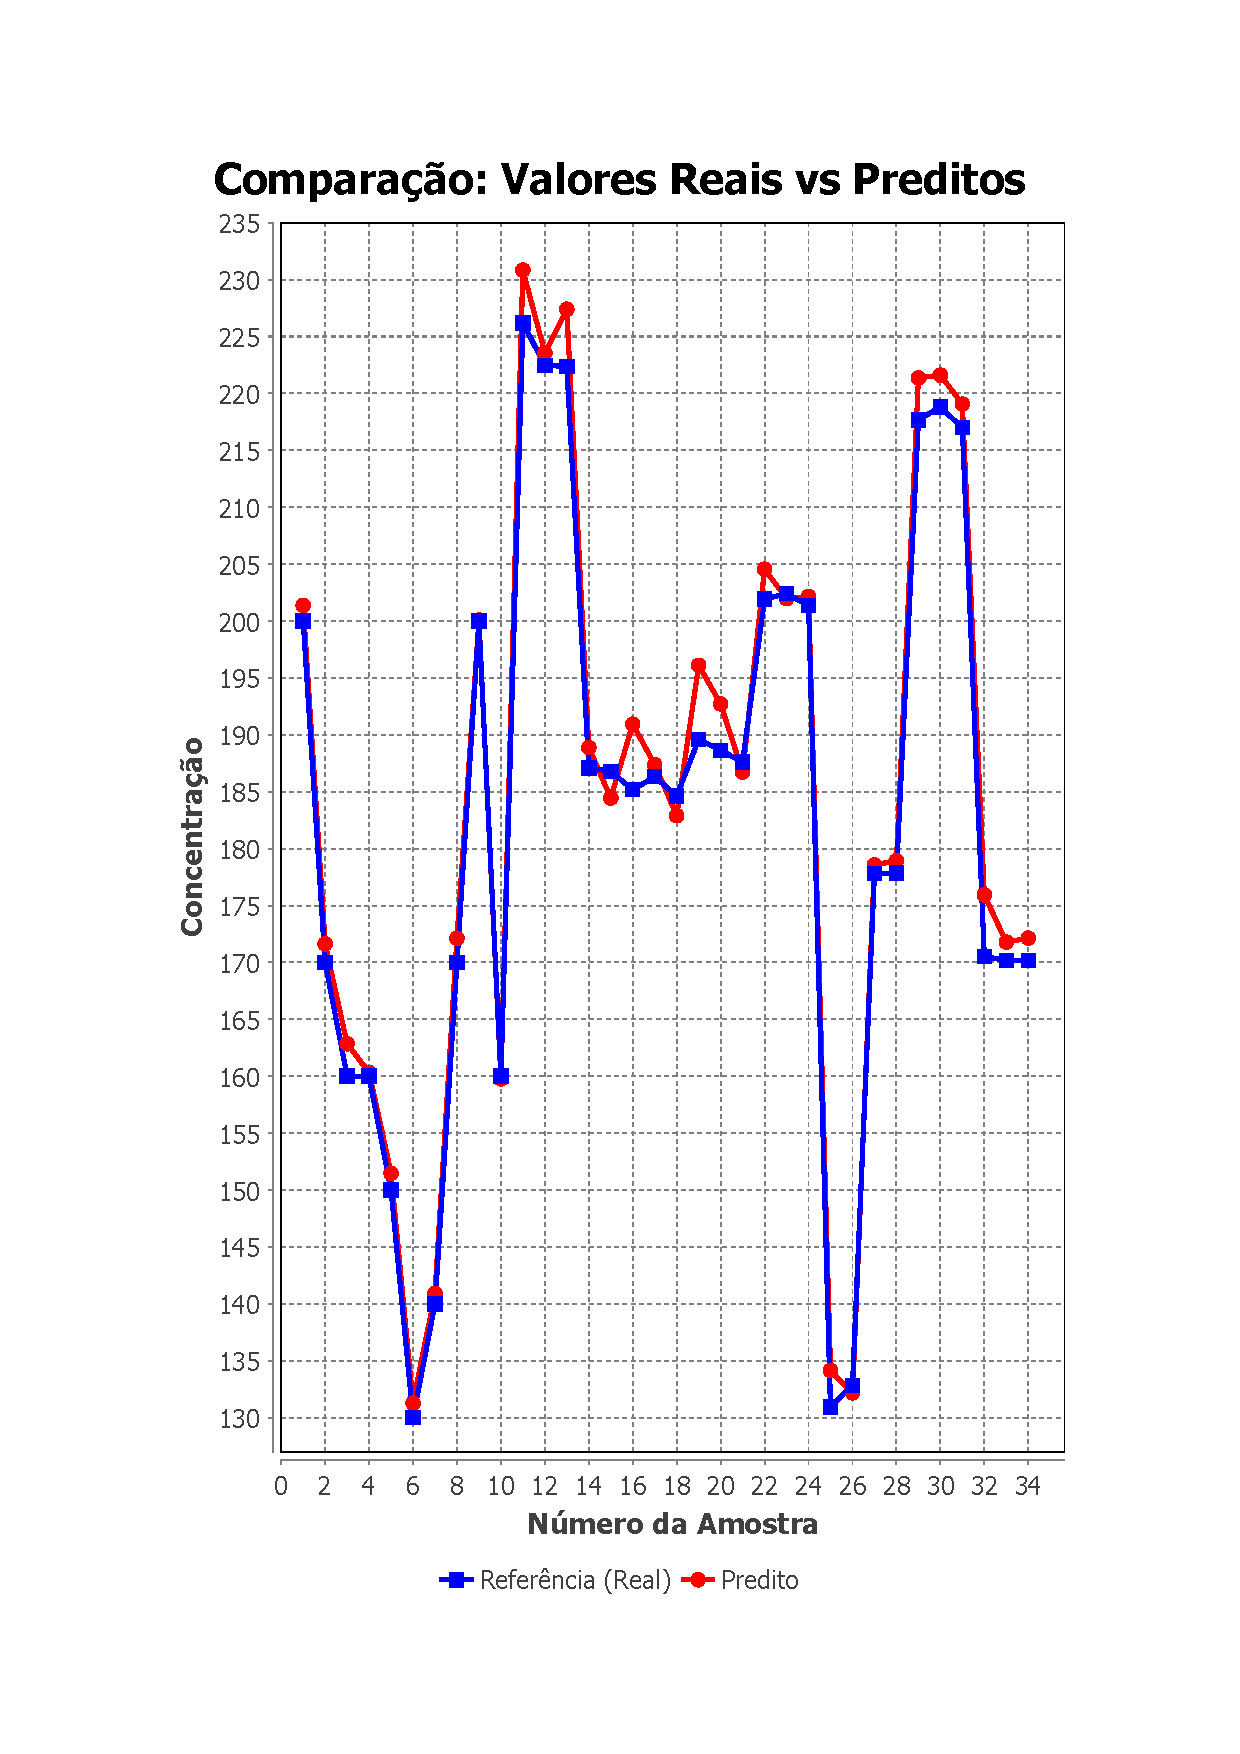
\includepdf[pages=-, scale=0.5]{./outros/fig/BootStrapRMSEPFe.pdf}  % Inclui todas as páginas
%--------------------------------------%Seção 5 - Requisitos Funcionais

\chapter{Engenharia de Software e Modernização}
\label{sec:engenhariasoftware}

\section{Engenharia de Requisitos com Sommerville}

Sommerville~\cite{sommerville2011} estrutura a engenharia de requisitos em quatro fases interdependentes: elicitação, análise, especificação e validação. A reestruturação do sistema em três módulos — \texttt{models.py}, \texttt{components.py} e \texttt{app.py} — evidencia como cada fase foi aplicada para preservar as regras de negócio do legado Vaadin/Java sem reaproveitar seu código-fonte.

\subsection{Elicitação}
As entradas críticas do domínio de regressão espectral foram identificadas diretamente no sistema Java original: as matrizes \texttt{Xcal} e \texttt{Xteste}, os vetores \texttt{Ycal} e \texttt{Yteste}, e os hiperparâmetros \textit{m} (número de \textit{bags}) e \textit{k} (fração de \textit{subagging}). O \texttt{app.py} captura esses insumos por meio de \texttt{st.file\_uploader} e \texttt{st.text\_input}, incluindo suporte a decimal com vírgula — particularidade do padrão brasileiro — tratada nas funções \texttt{parse\_matrix()} e \texttt{parse\_vector()} do \texttt{models.py}.

\subsection{Análise}
A análise revelou que a lógica do \texttt{RegressionService.java} podia ser decomposta em responsabilidades distintas: \textit{parse} de arquivos, algoritmos de regressão, métricas de avaliação e otimização por validação cruzada. Essa decomposição originou a estrutura modular adotada, onde \texttt{models.py} concentra toda a inteligência matemática, sem qualquer dependência de interface.

\subsection{Especificação}
As assinaturas de entrada e saída das principais funções do~\verb|models.py|~foram documentadas com \textit{type hints} \footnote{\textit{Type hints} são anotações opcionais da linguagem Python que declaram os tipos esperados dos parâmetros e do valor de retorno de uma função
(por exemplo, \texttt{x: np.ndarray} e \texttt{-> float}). Documentam a assinatura da função e permitem verificação estática por ferramentas externas, mas não são impostas pelo interpretador em tempo de execução.} nas principais funções do \texttt{models.py}:
\texttt{parse\_matrix(file\_obj) -> np.ndarray} e
\texttt{parse\_vector(file\_obj) -> np.ndarray}, em que \texttt{file\_obj} é um
objeto de arquivo (\textit{file-like}) que expõe \texttt{.name} e \texttt{.read()},
sendo a extensão (\texttt{.txt}, \texttt{.csv} ou \texttt{.xlsx}) usada para
escolher o \textit{parser};
\texttt{perform\_rlm(Xcal, Ycal, Xteste: np.ndarray) -> np.ndarray};
\texttt{calc\_metrics(actual, predicted) -> tuple[float, float, float]}.
A função \texttt{run\_full\_analysis()} retorna um dicionário (\texttt{dict})
com as chaves \texttt{log}, \texttt{optimal}, \texttt{metrics} e \texttt{preds},
definindo a interface de comunicação entre a camada de negócio e a camada de apresentação.

\subsection{Validação}
A validação cruzada 5-\textit{fold} implementada em \texttt{run\_cross\_validation()} opera como mecanismo de validação de equivalência, permitindo comparar o desempenho do sistema Python com os resultados históricos do sistema Java. O \textit{log} estruturado gerado por \texttt{run\_full\_analysis()} documenta cada etapa — dimensões detectadas, $\text{RMSEP}_{\text{CV}}$ por combinação de hiperparâmetros, métricas finais e tempo de execução — possibilitando auditoria científica e rastreabilidade completa. Para assegurar a estabilidade dessa arquitetura, construiu-se uma suíte com 92 testes automatizados, composta por 21 testes unitários, 60 testes de caixa-preta e 11 testes de carga e estresse.

\section{Arquitetura Modular em Python/Streamlit}

A arquitetura do sistema modernizado adota o padrão de separação de responsabilidades em três camadas físicas distintas, representadas pelos arquivos \texttt{models.py}, \texttt{components.py} e \texttt{app.py}. Essa organização substitui a estrutura monolítica do sistema Java original, garantindo testabilidade isolada e desacoplamento entre a lógica de negócio e a interface com o usuário.

O módulo \texttt{models.py} atua como a lógica matemática do sistema, encapsulando todas as operações matemáticas e estatísticas sem qualquer importação de bibliotecas de interface gráfica. Ele contém as implementações da RLM via \texttt{np.linalg.lstsq}, do \textit{bagging} e do \textit{subagging} parametrizados, das funções de \textit{parsing} de dados e das rotinas de validação cruzada 5-\textit{fold} com \textit{grid search}.

Ressalta-se que o sistema Java legado calcula os coeficientes da RLM pela
pseudoinversa de Moore-Penrose explícita (\texttt{SimpleMatrix.pseudoInverse()},
biblioteca EJML, implementada em Java puro), ao passo que a versão Python emprega
\texttt{np.linalg.lstsq}, que delega ao NumPy a rotina \texttt{gelsd} da
biblioteca LAPACK~\cite{anderson1999lapack}. Essa rotina resolve o problema de mínimos quadrados por
decomposição em valores singulares (SVD) e retorna a solução de mínima norma.
Para os sistemas subdeterminados deste trabalho ($17 \times 723$), ambas as
rotinas convergem para a mesma solução teórica
$\widehat{\boldsymbol{\beta}} = \mathbf{X}^{+}\mathbf{y}$, embora por caminhos
numéricos distintos.

O módulo \texttt{components.py} responde pela fábrica de componentes visuais e geração de gráficos interativos utilizando a biblioteca Plotly. Ele transforma as matrizes de resultados e vetores de predição retornados pela camada de modelagem em objetos de figura prontos para renderização, isolando o código de visualização do fluxo principal da aplicação.

O módulo \texttt{app.py} funciona como controlador da interface e do estado da sessão (\texttt{st.session\_state}). Ele captura as interações do usuário, invoca as funções puras de \texttt{models.py}, repassa os resultados para \texttt{components.py} e gerencia a exibição sequencial em abas. Essa divisão garante que alterações na camada visual não impactem os algoritmos científicos e vice-versa.

%A Figura~\ref{fig:arquitetura_python} apresenta as três camadas do sistema modernizado, em contraste com a organização monolítica do sistema Java original, ilustrada na Figura~\ref{fig:arquitetura_java}. O diagrama de classes dos módulos (Figura~\ref{fig:BaggingOptimized_classe3}) e os demais diagramas \gls{UML} estão reunidos no Apêndice~\ref{cha:testesgraficos}.

A Figura~\ref{fig:arquitetura_java} mostra a organização lógica em camadas do sistema Java original, contida em um único arquivo, e a Figura~\ref{fig:arquitetura_python} apresenta as três camadas físicas do sistema modernizado. O diagrama de classes dos módulos (Figura~\ref{fig:BaggingOptimized_classe3}) e os demais diagramas \gls{UML} estão no Apêndice~\ref{cha:testesgraficos}.

\begin{figure}[H]
    \caption{Organização lógica em camadas dentro de um único arquivo --- Sistema legado monolítico (Java Desktop).}
    \centering
    \begin{tikzpicture}[
        layer/.style={draw, rounded corners, minimum width=8cm,
                      minimum height=1.2cm, align=center, fill=#1},
        arrow/.style={-{Stealth}, thick}
    ]
        \node[layer=blue!15] (view) {Camada de Apresentação\\\texttt{Swing/AWT} (\texttt{JFrame}, \texttt{JPanel}, \textit{listeners})};
        \node[layer=green!15, below=0.8cm of view] (controller) {Camada de Controle\\Orquestração de eventos (\texttt{ActionListener})};
        \node[layer=orange!15, below=0.8cm of controller] (model) {lógica matemática\\\texttt{BaggingOptimized.java} + EJML (\texttt{SimpleMatrix})};

        \draw[arrow] (view) -- (controller);
        \draw[arrow] (controller) -- (model);
    \end{tikzpicture}
    \caption*{Fonte: \oautor}
    \label{fig:arquitetura_java}
\end{figure}

\begin{figure}[H]
    \caption{Arquitetura em camadas --- Sistema modernizado (Python/Streamlit).}
    \centering
    \begin{tikzpicture}[
        layer/.style={draw, rounded corners, minimum width=8cm,
                      minimum height=1.2cm, align=center, fill=#1},
        arrow/.style={-{Stealth}, thick}
    ]
        \node[layer=blue!15] (apresentacao) {Camada de Apresentação\\\texttt{app.py} --- Streamlit (orquestração de UI e sessão)};
        \node[layer=green!15, below=0.8cm of apresentacao] (visual) {Camada de Visualização\\\texttt{components.py} --- Plotly (fábrica de gráficos)};
        \node[layer=orange!15, below=0.8cm of visual] (nucleo) {lógica matemática\\\texttt{models.py} --- NumPy (\texttt{np.linalg.lstsq})};

        \draw[arrow] (apresentacao) -- (visual);
        \draw[arrow] (visual) -- (nucleo);
    \end{tikzpicture}
    \caption*{Fonte: \oautor}
    \label{fig:arquitetura_python}
\end{figure}

%Seção 6 - Engenharia de Software e Modernização

\chapter{Resultados e Discussões}
\label{sec:resultados}

\section{Avaliação Preditiva e Eficiência Computacional}

A avaliação experimental do sistema modernizado foi conduzida utilizando os dados espectrométricos de cinco analitos (Mn, Mo, Cr, Ni e Fe) presentes em amostras de aço-ligas. Os modelos de Regressão Linear Múltipla (RLM), RLM-\textit{bagging} e RLM-\textit{subagging} foram comparados quanto à acurácia preditiva, mensurada pelas métricas RMSEP, MAE e $R^2$, e quanto ao tempo de processamento computacional.

Para o Molibdênio (Mo) e o Cromo (Cr), a RLM clássica obteve menor RMSEP, indicando que a introdução das estratégias de \textit{ensemble} não proporcionou ganho de acurácia preditiva no conjunto de teste avaliado. Os resultados detalhados demonstram que a estrutura linear simples da RLM foi suficiente para capturar a variabilidade desses elementos sem introduzir a variância adicional inerente ao processo de reamostragem.

No caso do Ferro (Fe), o modelo RLM-\textit{bagging} apresentou o menor erro de predição, enquanto para o Manganês (Mn) e o Níquel (Ni), o RLM-\textit{subagging} obteve desempenho superior ou equivalente às demais abordagens. O desempenho diferenciado entre os analitos reflete suas características espectrais individuais no conjunto de dados. A verificação detalhada das causas físico-químicas subjacentes e a decomposição formal de viés e variância constituem tópicos sugeridos para investigações futuras.

Em termos de eficiência computacional, o RLM-\textit{subagging} demonstrou tempos de execução sistematicamente inferiores aos do RLM-\textit{bagging} em quatro dos cinco analitos avaliados. Essa redução do tempo de processamento é atribuída ao menor tamanho da amostra utilizada em cada submodelo durante o procedimento de \textit{subagging} ($k < 1$), o que diminui o custo computacional do ajuste de matrizes por Mínimos Quadrados Ordinários (MQO).%Seção 7 - Resultados e Discussões

\chapter{Interface e Experiência do Usuário (UI/UX) Científica}
\label{sec:uiux}

\section{Design da Interface e Fluxo de Trabalho}

A interface gráfica do sistema modernizado foi desenvolvida sobre o \textit{framework} Streamlit, adotando princípios de usabilidade voltados para aplicações científicas e de análise de dados. A organização visual busca minimizar a poluição de tela e guiar o usuário de forma intuitiva pelas etapas do processo de calibração multivariada.

A aplicação é dividida em três abas sequenciais que espelham o fluxo de trabalho do usuário:
\begin{enumerate}[label=\alph*)]
    \item \textbf{Aba 1 (Configuração e Carga de Dados):} Destinada ao envio dos arquivos de calibração e teste nos formatos \texttt{.txt}, \texttt{.csv} ou \texttt{.xlsx}, e à definição dos hiperparâmetros de entrada (número de replicações \textit{m} e fração de subamostragem \textit{k});
    \item \textbf{Aba 2 (Resultados Numéricos e Logs):} Exibe as métricas de avaliação preditiva (RMSEP, MAE, $R^2$), a indicação dos parâmetros ótimos selecionados pela validação cruzada 5-\textit{fold} e o \textit{log} detalhado de execução;
    \item \textbf{Aba 3 (Visualização Gráfica):} Apresenta os gráficos interativos gerados via Plotly, incluindo os gráficos de paridade (Valores Reais \textit{versus} Preditos) e as superfícies de erro.
\end{enumerate}

Essa estrutura em abas sequenciais organiza o \textit{workflow} analítico segundo as etapas operacionais do usuário, reduzindo a dispersão visual e delimitando os passos de execução.

O ambiente de implantação viabiliza o acesso simultâneo via navegador sem necessidade de instalação local de dependências ou ambientes de execução Java, sujeitando-se aos limites de concorrência e memória da plataforma de hospedagem adotada.%Seção 8 - Interface e Experiência do Usuário (UI/UX) Científica

% =============================================================================
\chapter{Interface e Experiência do Usuário (UI/UX) Científica}

\section{Design Centrado em Dados}

A interface do \texttt{app.py} organiza o fluxo analítico de forma hierárquica,
priorizando a clareza e a produtividade do cientista em detrimento de elementos
decorativos. A distribuição dos elementos entre abas, colunas e área central segue
princípios de design centrado no usuário, com decisões arquiteturais explícitas sobre
onde cada tipo de conteúdo deve residir.

\begin{description}

\item[a)] \textbf{Navegação por Etapas (\texttt{st.tabs})}: As três abas —
\textbf{Configuração}, \textbf{Resultados} e \textbf{Gráficos} — guiam o usuário em um
fluxo linear e irreversível: entrada de dados $\rightarrow$ execução $\rightarrow$
inspeção de resultados. Essa estrutura espelha o \textit{workflow} típico de validação de
modelos quimiométricos e reduz a sobrecarga cognitiva ao esconder informações irrelevantes
para a etapa atual.

\item[b)] \textbf{Layout em Colunas e Hierarquia Visual}: O \texttt{app.py} utiliza
\texttt{st.columns(2)} para agrupar uploads de calibração e teste lado a lado,
sinalizando visualmente a paridade entre os conjuntos. A área central é reservada para
cards de métricas gerados por \texttt{components.metric\_card\_html()} e para a tabela
comparativa em \texttt{pd.DataFrame}. O CSS centralizado em \texttt{components.APP\_CSS}
— incluindo gradientes de fundo, bordas coloridas por modelo e estilo terminal para o
log — replica dashboards técnicos e industriais sem poluir o \texttt{app.py} com
definições de estilo.

\item[c)] \textbf{Feedback Progressivo}: O botão \textbf{Executar Análise} é
desabilitado (\texttt{disabled=not files\_ok}) enquanto algum dos quatro arquivos estiver
ausente, prevenindo execuções inválidas. A barra de progresso atualizada pelo callback e
a mensagem \texttt{st.success} ao término fornecem confirmação clara de conclusão,
padrão recomendado pelas diretrizes de usabilidade para interfaces científicas.

\item[d)] \textbf{Decisão Arquitetural: \texttt{st.tabs} vs.\ \texttt{st.sidebar}}: O
Streamlit oferece dois paradigmas de organização de parâmetros técnicos e resultados:
a \texttt{st.sidebar} (painel lateral persistente, visível em todas as telas) e o
\texttt{st.tabs} (abas sequenciais que segmentam o fluxo). Para o perfil de usuário
científico deste sistema — que opera em etapas ordenadas e não retorna aos parâmetros
após a execução — o modelo de abas foi preferido por três razões: (1) impõe
explicitamente a sequência \textit{Configuração $\rightarrow$ Resultados $\rightarrow$
Gráficos}, prevenindo execuções prematuras; (2) preserva a área central integralmente
para visualização de resultados e gráficos, sem que uma barra lateral compita com os
gráficos do Plotly em largura de tela; e (3) alinha-se ao padrão de \textit{wizards}
adotado em \textit{softwares} de análise científica (Origin, MATLAB App Designer), nos
quais cada etapa revela seu conteúdo apenas quando os pré-requisitos anteriores foram
cumpridos. A \texttt{st.sidebar} permanece como alternativa recomendada para versões
futuras que implementem parâmetros globais persistentes, como configuração de idioma,
normalização de dados ou seleção de paleta de cores para publicação.

\end{description}

% ─────────────────────────────────────────────────────────────────────────────
\section{Visualização Interativa com Plotly}

A escolha do Plotly no \texttt{components.py} é fundamentada pela necessidade de
inspeção técnica precisa em espectrometria e regressão multimodelo.

\begin{description}

\item[a)] \textbf{Integração Nativa e Centralizada}: Com a separação em
\texttt{components.py}, todas as configurações visuais — cores por modelo
(\texttt{COR\_RLM}, \texttt{COR\_BAGGING}, \texttt{COR\_SUBAGGING}), estilos de eixo
(\texttt{\_AXIS\_STYLE}), cores de fundo (\texttt{\_PLOT\_BG}) — estão definidas em um
único arquivo. Alterar a paleta de cores ou o estilo de grade para padrões de publicação
científica requer modificação em um só lugar, sem tocar no \texttt{app.py} ou no
\texttt{models.py}.

\item[b)] \textbf{Ferramentas de Inspeção Científica}: Os gráficos \texttt{go.Scatter}
gerados por \texttt{build\_chart()} e \texttt{build\_scatter\_chart()} habilitam zoom,
\textit{pan}, \textit{hover} com coordenadas exatas e legendas interativas. A linha ideal
\textit{y=x} (\texttt{mode="lines", dash="dot"}) no gráfico de dispersão
(\texttt{build\_scatter\_chart}) permite validação visual imediata de viés e dispersão
dos três modelos sobrepostos — RLM Simples, Bagging e Subagging — em uma única figura.

\item[c)] \textbf{Padrões de Publicação}: Os eixos customizados (\texttt{showgrid=True},
\texttt{gridcolor="\#000000"}, fontes pretas explícitas via \texttt{\_AXIS\_STYLE})
garantem legibilidade para relatórios técnicos, apresentações e submissão a periódicos,
alinhando-se às normas de visualização de dados científicos sem exigir pós-processamento
externo das figuras.

\end{description}

% ─────────────────────────────────────────────────────────────────────────────
\section{Contratos de Interface e Funções}
\label{sec:contratos}

A separação em três módulos aplica rigorosamente o princípio de separação de
responsabilidades, tornando o sistema testável, manutenível e extensível
independentemente em cada camada.

\begin{description}

\item[a)] \textbf{Separação de Camadas}: O \texttt{models.py} não importa
\texttt{streamlit} nem \texttt{plotly}. O \texttt{components.py} não importa
\texttt{streamlit} nem \texttt{numpy}. O \texttt{app.py} não contém nenhuma função
matemática — a instrução mais complexa é a chamada \texttt{result =
run\_full\_analysis(...)}. Essa separação permite testar o \texttt{models.py}
isoladamente com \texttt{pytest} e dados sintéticos, sem instanciar nenhum componente de
interface.

\item[b)] \textbf{Contratos Explícitos via \textit{Type Hints}}: Todas as funções do
\texttt{models.py} declaram tipos de entrada e saída:
\texttt{perform\_bagging(...) -> np.ndarray},
\texttt{calc\_metrics(...) -> tuple[float, float, float]},
\texttt{find\_optimal\_parameters(...) -> tuple[dict, str]}.
No \texttt{app.py}, \texttt{parse\_int\_list()} e \texttt{parse\_float\_list()} lançam
\texttt{ValueError} com mensagens orientativas para entradas fora do domínio válido —
inteiros positivos para \textit{m} e decimais em $(0,1]$ para \textit{k} — prevenindo
falhas silenciosas na camada de negócio.

\item[c)] \textbf{Manutenibilidade e Escalabilidade}: Adicionar um novo modelo preditivo
(como Ridge Regression ou Random Forest) requer apenas uma nova função em
\texttt{models.py} e um novo bloco de exibição em \texttt{app.py}. Modificar a paleta de
cores ou o layout dos gráficos requer apenas alterações em \texttt{components.py}.
Nenhuma dessas mudanças impacta as outras camadas, confirmando que a arquitetura modular
adotada atende ao critério de \textbf{abertura para extensão, fechamento para
modificação} (\textit{Open/Closed Principle}) proposto por Robert C.
Martin~\cite{martin2008}.

\end{description}
%Seção 9 - Desenvolvimento Iterativo por Sprints e Validação por Testes Automatizados

\chapter{Conclusão}
\label{cha:conclusao}
\index{Conclusão}

Este estudo investiga, em caráter exploratório, as técnicas de
reamostragem \textit{bootstrap}, \textit{bagging} e \textit{subagging}
aplicadas à Regressão Linear Múltipla (RLM) na calibração multivariada
de amostras de aço-ligas. O trabalho implementa as abordagens
utilizando a RLM como modelo base e atende aos objetivos propostos,
dentro das limitações discutidas ao final desta seção.

%Os experimentos seguem um protocolo controlado, com a otimização dos hiperparâmetros por validação cruzada 5-\textit{fold} aplicada exclusivamente ao conjunto de calibração. Esse protocolo busca assegurar comparações justas e reprodutíveis entre a \textit{RLM clássica}, o \textit{RLM-bagging} e o \textit{RLM-subagging}. Além do RMSEP, o estudo incorpora as métricas \gls{MAE} e R$^2$, ampliando acaracterização do desempenho preditivo de cada técnica. Ressalta-se que as conclusões a seguir se referem a esse protocolo com otimização por validação cruzada: nos experimentos anteriores, com parâmetros fixados sem otimização formal, a técnica vencedora em alguns analitos (Ni e Fe) foi outra. Isso reforça que o desempenho relativo depende da forma como $m$ e $k$ são selecionados.

Os experimentos seguem um protocolo controlado, com a otimização dos
hiperparâmetros por validação cruzada 5-\textit{fold} aplicada
exclusivamente ao conjunto de calibração. Esse protocolo busca
assegurar comparações justas e reprodutíveis entre a \textit{RLM
clássica}, o \textit{RLM-bagging} e o \textit{RLM-subagging}. Além do
RMSEP, o estudo incorpora as métricas \gls{MAE} e R$^2$, ampliando a
caracterização do desempenho preditivo de cada técnica.

Ressalta-se que as conclusões a seguir se referem a esse protocolo com 
otimização por validação cruzada: nos experimentos anteriores, com 
parâmetros fixados sem otimização formal, a técnica vencedora em alguns 
analitos (Ni e Fe) foi outra. Isso reforça que o desempenho relativo 
depende da forma como $m$ e $k$ são selecionados.

%----------------------------------------------------------------------------

A análise comparativa revela variações de desempenho dependentes do
analito e indica, para este conjunto de dados específico, a
inexistência de uma técnica universalmente superior. Para o Manganês
(Mn), o RLM-\textit{subagging} ($k^* = 80\%$, $m^* = 10$) apresenta o
menor RMSEP (0,0966), uma redução de 8,1\% em relação à RLM clássica.
Para o Ferro (Fe), o RLM-\textit{bagging} ($m^* = 30$) obtém o melhor
desempenho (RMSEP = 2,6406), com melhoria de 4,0\% sobre a RLM
clássica.

Para o Níquel (Ni), o RLM-\textit{subagging} ($k^* = 60\%$,
$m^* = 10$) exibe resultado marginalmente superior (RMSEP = 1,6003),
com diferença de 0,25\% em relação à RLM clássica. Dada a magnitude
dessa diferença e o tamanho amostral disponível, o resultado deve ser
interpretado com cautela. Em contrapartida, para o Molibdênio (Mo) e o
Cromo (Cr), a RLM clássica apresenta desempenho superior (RMSEP de
0,2633 e 1,0798, respectivamente), indicando que a complexidade
adicional das estratégias de \textit{ensemble} não resulta em ganho de
precisão para esses analitos neste contexto.

%---------------------------------------------------------------------

A avaliação por meio do RMSEP, complementada pelo \gls{MAE} e pelo
R$^2$, permite uma caracterização abrangente do desempenho preditivo.
Todos os modelos apresentam coeficiente de determinação superior a
0,98 para todos os elementos, o que evidencia elevada capacidade
preditiva para o conjunto de dados analisado.

Para Mn e Ni, o RLM-\textit{subagging} apresenta dominância de Pareto
sobre o RLM-\textit{bagging}, por ser simultaneamente superior em
acurácia (RMSEP e \gls{MAE}) e mais eficiente computacionalmente, o
que reforça sua indicação nesses dois casos. Para Mo e Cr, os
resultados sustentam a adoção da RLM clássica, em razão de sua
simplicidade e de sua eficiência computacional.

%--------------------------------------------------------------------

A análise da eficiência computacional mostra diferenças expressivas
entre os métodos. A RLM clássica é a abordagem mais rápida em todos
os analitos. O RLM-\textit{subagging} ocupa posição intermediária:
tomando a razão entre os tempos do RLM-\textit{bagging} e do
RLM-\textit{subagging} em cada analito, o subagging é, em média, 3,0
vezes mais rápido, com variação entre 1,4 vez (Mo) e 6,3 vezes (Ni).
Em termos agregados, a soma dos tempos dos cinco analitos é cerca de
53\% menor no subagging.

Em relação à RLM clássica, o RLM-\textit{subagging} apresenta custo de
até 19,5 vezes superior, enquanto o RLM-\textit{bagging} é, em média,
22,1 vezes mais lento. O Cromo (Cr) é o único caso em que o
RLM-\textit{subagging} não apresenta vantagem temporal sobre o
RLM-\textit{bagging}, comportamento explicado pelo maior número de
replicações selecionado por validação cruzada ($m^* = 30$ contra
$m^* = 20$).

%-------------------------------------------------------------------------

A investigação indica que o RLM-\textit{subagging} é a alternativa
mais equilibrada entre precisão e eficiência para os dados analisados,
sendo recomendado para Mn e Ni. Para Mo e Cr, os resultados sustentam
a adoção da RLM clássica. O RLM-\textit{bagging} mostra-se preferível
para Fe, embora o RLM-\textit{subagging} atinja desempenho preditivo
equivalente (RMSEP de 2,6509 e R$^2$ idêntico, 0,9900) em menos da
metade do tempo. A relação de compromisso entre acurácia e tempo atua
como elemento decisivo na seleção da técnica.

% Do ponto de vista da engenharia de software, o trabalho atinge seus objetivos específicos. A arquitetura modular em três camadas independentes (\texttt{models.py}, \texttt{components.py} e \texttt{app.py}) satisfaz o requisito de modularidade (RNF01). A suíte de 92 testes automatizados atesta a equivalência entre o sistema Python e o sistema Java legado (RNF03) em dois níveis distintos: para a RLM, que é determinística, a equivalência numérica é estrita (tolerância de $5\times10^{-4}$ em RMSEP, \gls{MAE} e R$^2$); para o \textit{bagging} e o \textit{subagging}, que são estocásticos e cujas sequências pseudoaleatórias diferem entre Python e Java, a suíte verifica consistência estatística dentro de tolerâncias mais amplas (0,15 em RMSEP e \gls{MAE}; $5\times10^{-3}$ em R$^2$). Assim, a migração incremental orientada por testes de caixa-preta constitui contribuição metodológica válida independentemente do domínio de aplicação, ainda que não demonstre identidade das reamostragens entre as duas implementações.

Do ponto de vista da engenharia de software, o trabalho atinge seus
objetivos específicos. A arquitetura modular em três camadas
independentes (\texttt{models.py}, \texttt{components.py} e
\texttt{app.py}) satisfaz o requisito de modularidade (RNF01). A suíte
de 92 testes automatizados atesta a equivalência entre o sistema
Python e o sistema Java legado (RNF03) em dois níveis distintos.

Para a RLM, que é determinística, a equivalência numérica é estrita,
com tolerância de $5\times10^{-4}$ em RMSEP, \gls{MAE} e R$^2$. Para o
\textit{bagging} e o \textit{subagging}, que são estocásticos e cujas
sequências pseudoaleatórias diferem entre Python e Java, a suíte
verifica consistência estatística dentro de tolerâncias mais amplas:
0,15 em RMSEP e \gls{MAE}; $5\times10^{-3}$ em R$^2$.

Assim, a migração incremental orientada por testes de caixa-preta
constitui contribuição metodológica válida independentemente do
domínio de aplicação. Entretanto, essa abordagem não demonstra
identidade das reamostragens entre as duas implementações.

%Este estudo apresenta limitações pertinentes. O conjunto de dados corresponde a uma composição específica de aço-liga, analisada sob condições instrumentais particulares, o que restringe a extrapolação dos achados para outras composições, regimes amostrais ou configurações espectrométricas. A razão de aproximadamente 42 preditores por observação no conjunto de calibração (723 variáveis para 17 amostras) caracteriza um regime de alta dimensionalidade que, embora tratável pela pseudo-inversa de Moore-Penrose, amplifica a sensibilidade dos resultados à composição das amostras disponíveis. Os \textit{folds} da validação cruzada contêm apenas três ou quatro amostras, o que limita a estabilidade da seleção de $m^*$ e $k^*$.

Este estudo apresenta limitações pertinentes. O conjunto de dados
corresponde a uma composição específica de aço-liga, analisada sob
condições instrumentais particulares, o que restringe a extrapolação
dos achados para outras composições, regimes amostrais ou
configurações espectrométricas.

A razão de aproximadamente 42 preditores por observação no conjunto
de calibração (723 variáveis para 17 amostras) caracteriza um regime
de alta dimensionalidade. Embora tratável pela pseudo-inversa de
Moore-Penrose, esse cenário amplifica a sensibilidade dos resultados
à composição das amostras disponíveis.

Além disso, os \textit{folds} da validação cruzada contêm apenas três
ou quatro amostras, o que limita a estabilidade da seleção de $m^*$ e
$k^*$.

% Outras limitações são de natureza metodológica. O valor $k^* = 80\%$ coincide com o limite superior da grade avaliada ($k \in \{0{,}50;\ 0{,}60;\ 0{,}70;\ 0{,}80\}$) em quatro dos cinco analitos, de modo que o ótimo real pode situar-se em frações maiores. As tolerâncias adotadas nos testes de caixa-preta dos métodos estocásticos são amplas em relação às diferenças de desempenho entre as técnicas, de modo que a suíte assegura consistência estatística, mas não discrimina implementações com desempenhos próximos. Por fim, a análise adota exclusivamente a RLM como modelo base.

Outras limitações são de natureza metodológica. O valor $k^* = 80\%$
coincide com o limite superior da grade avaliada
($k \in \{0{,}50;\ 0{,}60;\ 0{,}70;\ 0{,}80\}$) em quatro dos cinco
analitos, de modo que o ótimo real pode situar-se em frações maiores.

As tolerâncias adotadas nos testes de caixa-preta dos métodos
estocásticos são amplas em relação às diferenças de desempenho entre
as técnicas. Desse modo, a suíte assegura consistência estatística,
mas não discrimina implementações com desempenhos próximos.

Por fim, a análise adota exclusivamente a RLM como modelo base.


% Como direcionamento para investigações futuras, este estudo recomenda a expansão do escopo para conjuntos amostrais maiores e diferentes classes de materiais, a ampliação da grade de $k$ além de 80\% e a comparação com modelos preditivos alternativos, como \gls{PLS}, \gls{LASSO} e redes neurais, que permitirão avaliar se os padrões observados se sustentam em regimes mais generalizáveis. Recomenda-se ainda o uso de uma mesma sequência de reamostragens (por exemplo, índices exportados pelo Java e lidos pelo Python) para permitir a comparação amostra a amostra dos métodos estocásticos, e a avaliação de técnicas de \textit{ensemble} mais sofisticadas, como \textit{boosting} e \textit{stacking}.

Como direcionamento para investigações futuras, este estudo recomenda
a expansão do escopo para conjuntos amostrais maiores e diferentes
classes de materiais, a ampliação da grade de $k$ além de 80\% e a
comparação com modelos preditivos alternativos, como \gls{PLS},
\gls{LASSO} e redes neurais. Essas abordagens permitirão avaliar se os
padrões observados se sustentam em regimes mais generalizáveis.

Recomenda-se ainda o uso de uma mesma sequência de reamostragens
(por exemplo, índices exportados pelo Java e lidos pelo Python) para
permitir a comparação amostra a amostra dos métodos estocásticos.
Sugere-se também a avaliação de técnicas de \textit{ensemble} mais
sofisticadas, como \textit{boosting} e \textit{stacking}.



%Seção 10 - Conclusão

%% ============================================================
% Quadros de classificação das funções por tipo: Java e Python
% Inserir na Seção "Engenharia de Software e Modernização"
% Requer: tabularx, threeparttable, array, captionsetup
% ============================================================

O Quadro~\ref{tab:tipos_java} classifica por tipo as funções do sistema Java legado, concentradas em um único arquivo (\texttt{BaggingOptimized.java}). O Quadro~\ref{tab:tipos_python} apresenta a mesma classificação para o sistema Python, no qual as funções se distribuem entre os módulos \texttt{models.py}, \texttt{components.py} e \texttt{app.py}.

% ------------------------------------------------------------
% QUADRO 1 — TIPOS DE FUNÇÕES JAVA
% ------------------------------------------------------------
\begin{quadro}[ht]
\begin{center}
\footnotesize
\captionsetup{justification=centering, labelsep=endash, width=0.75\linewidth}
\caption{Tipos de funções do sistema Java legado.}
\label{tab:tipos_java}
\begin{threeparttable}
\renewcommand{\arraystretch}{1.15}
\begin{tabularx}{\textwidth}{|>{\raggedright\arraybackslash}p{3.2cm}|>{\raggedright\arraybackslash}X|>{\raggedright\arraybackslash}X|}
\hline
\textbf{Tipo} & \textbf{Funções} & \textbf{Responsabilidade} \\ \hline
Modelagem & \texttt{performRLM}, \texttt{performBagging}, \texttt{pseudoInverse} & Ajuste da RLM e dos \textit{ensembles} de \textit{bagging} e \textit{subagging} \\ \hline
Métricas de avaliação & \texttt{calculateMetrics}, \texttt{calculateRMSE}, \texttt{calculateMAE}, \texttt{calculateR2}, \texttt{calculateStdDev} & Cálculo de RMSEP, MAE, $R^2$ e desvio padrão \\ \hline
Validação cruzada e otimização & \texttt{optimizeBaggingParameters}, \texttt{optimizeSubaggingParameters}, \texttt{findOptimalParameters} & Validação cruzada 5-\textit{fold} e \textit{grid search} de $m$ e $k$ \\ \hline
Manipulação de matrizes & \texttt{extractRows}, \texttt{copyRow} & Extração e cópia de linhas de matrizes \\ \hline
Entrada e saída de dados & \texttt{loadMatrixFromFile}, \texttt{loadVectorFromFile}, \texttt{detectarDimensoes}, \texttt{contarLinhas}, \texttt{salvarResultados} & Leitura dos arquivos \texttt{.txt}, detecção de dimensões e gravação do relatório \\ \hline
Validação de parâmetros & \texttt{parseMValues}, \texttt{parseKValues} & Conversão e validação dos valores de $m$ e $k$ digitados \\ \hline
Interface gráfica & Construtor \texttt{BaggingOptimized}, \texttt{initComponents}, \texttt{criarPainelArquivo}, \texttt{selecionarArquivo}, \texttt{FileConsumer.accept} & Montagem da janela Swing, seleção de arquivos e \textit{callback} de seleção \\ \hline
Visualização & \texttt{plotComparison} & Gráfico de valores reais e preditos com JFreeChart \\ \hline
Orquestração e controle & \texttt{executarAnalise}, \texttt{main} & Execução da análise em \texttt{SwingWorker} e ponto de entrada da aplicação \\ \hline
\end{tabularx}
\begin{tablenotes}[flushleft]
\footnotesize
\item Fonte:~\oautor
\end{tablenotes}
\end{threeparttable}
\end{center}
\end{quadro}

% ------------------------------------------------------------
% QUADRO 2 — TIPOS DE FUNÇÕES PYTHON
% ------------------------------------------------------------
\begin{quadro}[ht]
\begin{center}
\footnotesize
\captionsetup{justification=centering, labelsep=endash, width=0.75\linewidth}
\caption{Tipos de funções do sistema Python/Streamlit.}
\label{tab:tipos_python}
\begin{threeparttable}
\renewcommand{\arraystretch}{1.15}
\begin{tabularx}{\textwidth}{|>{\raggedright\arraybackslash}p{2.8cm}|>{\raggedright\arraybackslash}p{2.4cm}|>{\raggedright\arraybackslash}X|>{\raggedright\arraybackslash}X|}
\hline
\textbf{Tipo} & \textbf{Módulo} & \textbf{Funções} & \textbf{Responsabilidade} \\ \hline
Modelagem & \texttt{models.py} & \texttt{perform\_rlm}, \texttt{perform\_bagging} & Ajuste da RLM e dos \textit{ensembles} via \texttt{np.linalg.lstsq} \\ \hline
Métricas de avaliação & \texttt{models.py} & \texttt{calc\_metrics} & Cálculo de RMSEP, MAE e $R^2$ \\ \hline
Validação cruzada e otimização & \texttt{models.py} & \texttt{run\_cross\_validation}, \texttt{find\_optimal\_parameters} & Validação cruzada 5-\textit{fold} e \textit{grid search} de $m$ e $k$ \\ \hline
Leitura de dados & \texttt{models.py} & \texttt{parse\_matrix}, \texttt{parse\_vector}, \texttt{\_file\_ext}, \texttt{\_detect\_csv\_sep} & Leitura de \texttt{.txt}, \texttt{.csv} e \texttt{.xlsx}, com detecção de extensão e de separador \\ \hline
Orquestração da análise & \texttt{models.py} & \texttt{run\_full\_analysis} & Otimização, avaliação final dos três modelos e geração do \textit{log} \\ \hline
Internacionalização & \texttt{models.py}, \texttt{components.py}, \texttt{app.py} & \texttt{\_tl}, \texttt{\_t} & Tradução de rótulos, \textit{log} e textos da interface (português e inglês) \\ \hline
Visualização e componentes & \texttt{components.py} & \texttt{build\_chart}, \texttt{build\_scatter\_chart}, \texttt{metric\_card\_html}, \texttt{get\_header\_html} & Gráficos Plotly, \textit{cards} de métricas e cabeçalho em HTML \\ \hline
Validação de parâmetros & \texttt{app.py} & \texttt{parse\_int\_list}, \texttt{parse\_float\_list} & Conversão e validação dos valores de $m$ e $k$ \\ \hline
Controle da interface & \texttt{app.py} & \texttt{update\_progress} & \textit{Callback} da barra de progresso (interface e abas em \textit{script} sequencial) \\ \hline
\end{tabularx}
\begin{tablenotes}[flushleft]
\footnotesize
\item Fonte:~\oautor
\item \textit{Nota:} O arquivo \texttt{app.py} é executado de forma sequencial pelo Streamlit; o layout, as abas e o estado de sessão são definidos no corpo do \textit{script}, e não em funções.
\end{tablenotes}
\end{threeparttable}
\end{center}
\end{quadro}

%\newpage
%% ============================================================
% Quadro de equivalência de funções: Java (legado) x Python
% Inserir na Seção "Engenharia de Software e Modernização"
% Requer: tabularx, threeparttable, array, captionsetup
% ============================================================

No Quadro~\ref{tab:equivalencia_funcoes} apresenta-se a correspondência entre as funções do sistema Java legado (\texttt{BaggingOptimized.java}) e suas equivalentes na reescrita em Python/Streamlit (\texttt{models.py}, \texttt{components.py} e \texttt{app.py}).

\begin{quadro}[ht]
\begin{center}
\footnotesize
\captionsetup{justification=centering, labelsep=endash, width=0.75\linewidth}
\caption{Equivalência entre as funções do sistema Java legado e do sistema Python.}
\label{tab:equivalencia_funcoes}
\begin{threeparttable}
\renewcommand{\arraystretch}{1.15}
\begin{tabularx}{\textwidth}{|>{\raggedright\arraybackslash}X|>{\raggedright\arraybackslash}X|}
\hline
\textbf{Função Java (\texttt{BaggingOptimized.java})} & \textbf{Função Python equivalente} \\ \hline
\texttt{performRLM(Xcal, Ycal, Xteste)} & \texttt{perform\_rlm(Xcal, Ycal, Xteste)} --- \texttt{models.py} \\ \hline
\texttt{performBagging(Xcal, Ycal, Xteste, numBags, withReplacement, sampleFraction)} & \texttt{perform\_bagging(Xcal, Ycal, Xteste, num\_bags, with\_replacement, fraction, seed)} --- \texttt{models.py} \\ \hline
\texttt{pseudoInverse(matrix)} & \texttt{np.linalg.lstsq(...)}, invocada em \texttt{perform\_rlm()} e \texttt{perform\_bagging()} \\ \hline
\texttt{calculateMetrics(actual, predicted, nanoTime)} & \texttt{calc\_metrics(actual, predicted)} --- \texttt{models.py}; o tempo é medido em \texttt{run\_full\_analysis()} com \texttt{time.perf\_counter()} \\ \hline
\texttt{calculateRMSE(actual, predicted)} & \texttt{calc\_metrics()} (retorno \texttt{rmse}) e cálculo direto em \texttt{run\_cross\_validation()} \\ \hline
\texttt{calculateMAE(actual, predicted)} & \texttt{calc\_metrics()} (retorno \texttt{mae}) \\ \hline
\texttt{calculateR2(actual, predicted)} & \texttt{calc\_metrics()} (retorno \texttt{r2}) \\ \hline
\texttt{calculateStdDev(values, mean)} & \texttt{np.std()}, invocada em \texttt{run\_cross\_validation()} \\ \hline
\texttt{optimizeBaggingParameters(Xcal, Ycal, m)} & \texttt{run\_cross\_validation(Xcal, Ycal, m, True, 1.0)} --- \texttt{models.py} \\ \hline
\texttt{optimizeSubaggingParameters(Xcal, Ycal, m, k)} & \texttt{run\_cross\_validation(Xcal, Ycal, m, False, k)} --- \texttt{models.py} \\ \hline
\texttt{findOptimalParameters(Xcal, Ycal, mValues, kValues, log)} & \texttt{find\_optimal\_parameters(Xcal, Ycal, m\_values, k\_values, progress\_callback, lang)} --- \texttt{models.py} \\ \hline
\texttt{executarAnalise()} (Etapas 1 a 3 no \texttt{SwingWorker}) & \texttt{run\_full\_analysis(Xcal, Ycal, Xteste, Yteste, m\_values, k\_values, progress\_cb, lang)} --- \texttt{models.py} \\ \hline
\texttt{extractRows(matrix, indices)} & Indexação NumPy (\texttt{Xcal[train\_idx]}, \texttt{Xcal[val\_idx]}) em \texttt{run\_cross\_validation()} \\ \hline
\texttt{copyRow(src, srcRow, dest, destRow)} & Indexação NumPy (\texttt{Xcal[idx]}) em \texttt{perform\_bagging()} \\ \hline
\texttt{Collections.shuffle(indices, new Random(42))} & \texttt{np.random.default\_rng(seed).permutation(n)} em \texttt{run\_cross\_validation()} \\ \hline
\texttt{loadMatrixFromFile(filename, rows, cols)} & \texttt{parse\_matrix(file\_obj)} --- \texttt{models.py} \\ \hline
\texttt{loadVectorFromFile(filename, rows)} & \texttt{parse\_vector(file\_obj)} --- \texttt{models.py} \\ \hline
\texttt{detectarDimensoes(file)} e \texttt{contarLinhas(file)} & Atributo \texttt{.shape} do \textit{array} NumPy, registrado no \textit{log} por \texttt{run\_full\_analysis()} \\ \hline
\texttt{parseMValues()} & \texttt{parse\_int\_list(text)} --- \texttt{app.py} \\ \hline
\texttt{parseKValues()} & \texttt{parse\_float\_list(text)} --- \texttt{app.py} \\ \hline
\texttt{salvarResultados(conteudo)} & \texttt{st.download\_button(...)} para o \textit{log} (\texttt{relatorio.txt}) e para as métricas (\texttt{metricas.csv}) --- \texttt{app.py} \\ \hline
\texttt{plotComparison(yteste, ypred, method)} (JFreeChart) & \texttt{build\_chart(y\_real, y\_pred, title, pred\_color, lang)} --- \texttt{components.py} (Plotly) \\ \hline
\texttt{initComponents()}, \texttt{criarPainelArquivo()} e \texttt{selecionarArquivo()} & \texttt{st.file\_uploader}, \texttt{st.text\_input} e \texttt{st.tabs} --- \texttt{app.py} \\ \hline
Campos \texttt{fileXcal}, \texttt{fileYcal}, \texttt{fileXteste}, \texttt{fileYteste} & \texttt{st.session\_state} --- \texttt{app.py} \\ \hline
Classes \texttt{CVResult}, \texttt{OptimalParams} e \texttt{FinalMetrics} & Tuplas e dicionários (\texttt{optimal}, \texttt{metrics}), sem classes dedicadas \\ \hline
\multicolumn{1}{|c|}{---} & \texttt{build\_scatter\_chart(preds, lang)} --- gráfico de dispersão Real $\times$ Predito (sem correspondente em Java) \\ \hline
\end{tabularx}
\begin{tablenotes}[flushleft]
\footnotesize
\item Fonte:~\oautor
\item \textit{Nota:} O sinal convencional --- indica que não há função equivalente no sistema Java.
\end{tablenotes}
\end{threeparttable}
\end{center}
\end{quadro}

%\newpage
%O Quadro~\ref{tab:equiv_nucleo} apresenta a correspondência entre as funções do núcleo matemático do sistema Java legado (\texttt{BaggingOptimized.java}) e as do módulo \texttt{models.py}. O Quadro~\ref{tab:equiv_interface} reúne as funções de interface, entrada e saída de dados, que na reescrita em Python/Streamlit se distribuem entre \texttt{models.py}, \texttt{components.py} e \texttt{app.py}.

\begingroup
\footnotesize
\renewcommand{\arraystretch}{1.15}
\setlength{\tabcolsep}{4pt}

\refstepcounter{quadro}
\addcontentsline{loq}{quadro}{\protect\numberline{\thequadro}Equivalência entre as funções do núcleo matemático: Java e Python}
\begin{center}
  \begin{minipage}{0.85\linewidth}
    \centering
    \quadroname~\thequadro~--~Equivalência entre as funções do núcleo matemático: Java e Python.
  \end{minipage}
\end{center}
\label{tab:equiv_nucleo}%tab:equiv_nucleo
\vspace{-0.3cm}

\begin{longtable}{|>{\raggedright\arraybackslash}p{0.46\textwidth}|>{\raggedright\arraybackslash}p{0.46\textwidth}|}
\hline
\textbf{Função Java (\texttt{BaggingOptimized.java})} & \textbf{Função Python equivalente} \\ \hline
\endfirsthead

\hline
\textbf{Função Java (\texttt{BaggingOptimized.java})} & \textbf{Função Python equivalente} \\ \hline
\endhead

\hline
\multicolumn{2}{r}{\footnotesize\textit{Continua na próxima página}} \\
\endfoot

\hline
\endlastfoot

% ---------- Núcleo matemático (models.py) ----------
\texttt{performRLM(Xcal, Ycal, Xteste)} & \texttt{perform\_rlm(Xcal, Ycal, Xteste)} em \texttt{models.py} \\ \hline
\texttt{performBagging(Xcal, Ycal, Xteste, numBags, withReplacement, sampleFraction)} & \texttt{perform\_bagging(Xcal, Ycal, Xteste, num\_bags, with\_replacement, fraction, seed)} \\ \hline
\texttt{pseudoInverse(matrix)} & \texttt{np.linalg.lstsq(...)}, invocada em \texttt{perform\_rlm()} e \texttt{perform\_bagging()} \\ \hline
\texttt{calculateMetrics(actual, predicted, nanoTime)} & \texttt{calc\_metrics(actual, predicted)}; o tempo é medido em \texttt{run\_full\_analysis()} com \texttt{time.perf\_counter()} \\ \hline
\texttt{calculateRMSE(actual, predicted)} & \texttt{calc\_metrics()} (retorno \texttt{rmse}) e cálculo direto em \texttt{run\_cross\_validation()} \\ \hline
\texttt{calculateMAE(actual, predicted)} & \texttt{calc\_metrics()} (retorno \texttt{mae}) \\ \hline
\texttt{calculateR2(actual, predicted)} & \texttt{calc\_metrics()} (retorno \texttt{r2}) \\ \hline
\texttt{calculateStdDev(values, mean)} & \texttt{np.std()}, invocada em \texttt{run\_cross\_validation()} \\ \hline
\texttt{optimizeBaggingParameters(Xcal, Ycal, m)} & \texttt{run\_cross\_validation(Xcal, Ycal, m, True, 1.0)} \\ \hline
\texttt{optimizeSubaggingParameters(Xcal, Ycal, m, k)} & \texttt{run\_cross\_validation(Xcal, Ycal, m, False, k)} \\ \hline
\texttt{findOptimalParameters(Xcal, Ycal, mValues, kValues, log)} & \texttt{find\_optimal\_parameters(Xcal, Ycal, m\_values, k\_values, progress\_callback, lang)} \\ \hline
\texttt{executarAnalise()} (Etapas 1 a 3 no \texttt{SwingWorker}) & \texttt{run\_full\_analysis(Xcal, Ycal, Xteste, Yteste, m\_values, k\_values, progress\_cb, lang)} \\ \hline
\texttt{extractRows(matrix, indices)} & Indexação NumPy (\texttt{Xcal[train\_idx]}, \texttt{Xcal[val\_idx]}) em \texttt{run\_cross\_validation()} \\ \hline
\texttt{copyRow(src, srcRow, dest, destRow)} & Indexação NumPy (\texttt{Xcal[idx]}) em \texttt{perform\_bagging()} \\ \hline
\texttt{Collections.shuffle(indices, new Random(42))} & \texttt{np.random.default\_rng(seed).permutation(n)} em \texttt{run\_cross\_validation()} \\ \hline
Classes \texttt{CVResult}, \texttt{OptimalParams} e \texttt{FinalMetrics} & Tuplas e dicionários (\texttt{optimal}, \texttt{metrics}), sem classes dedicadas \\ \hline

% ---------- Leitura e validação de dados ----------
\texttt{loadMatrixFromFile(filename, rows, cols)} & \texttt{parse\_matrix(file\_obj)} em \texttt{models.py}; lê \texttt{.txt}, \texttt{.csv} e \texttt{.xlsx}, sem exigir \texttt{rows} e \texttt{cols} \\ \hline
\texttt{loadVectorFromFile(filename, rows)} & \texttt{parse\_vector(file\_obj)} em \texttt{models.py}; lê \texttt{.txt}, \texttt{.csv} e \texttt{.xlsx} \\ \hline
\texttt{detectarDimensoes(file)} & Atributo \texttt{shape} do \texttt{np.ndarray} retornado por \texttt{parse\_matrix()}, registrado no \textit{log} por \texttt{run\_full\_analysis()} \\ \hline
\texttt{contarLinhas(file)} & \texttt{Ycal.shape[0]} e \texttt{Yteste.shape[0]} do vetor retornado por \texttt{parse\_vector()} \\ \hline
\texttt{parseMValues()} & \texttt{parse\_int\_list(text)} em \texttt{app.py} \\ \hline
\texttt{parseKValues()} & \texttt{parse\_float\_list(text)} em \texttt{app.py} \\ \hline

% ---------- Saída e visualização ----------
\texttt{salvarResultados(conteudo)} & \texttt{st.download\_button} em \texttt{app.py}, que exporta o \textit{log} (\texttt{relatorio.txt}) e as métricas (\texttt{metricas.csv}) sem gravar em disco no servidor \\ \hline
\texttt{plotComparison(yteste, ypred, method)} & \texttt{build\_chart(y\_real, y\_pred, title, pred\_color, lang)} em \texttt{components.py}, complementada por \texttt{build\_scatter\_chart(preds, lang)} \\ \hline

% ---------- Interface ----------
\texttt{initComponents()} & Bloco de layout de \texttt{app.py}: \texttt{st.tabs()}, \texttt{get\_header\_html()} e \texttt{APP\_CSS} (\texttt{components.py}) \\ \hline
\texttt{criarPainelArquivo(label, textField, action)} & Trecho de \texttt{app.py} que combina \texttt{st.markdown()} (rótulo e descrição), \texttt{st.file\_uploader()} e \texttt{st.expander()} para cada arquivo \\ \hline
\texttt{selecionarArquivo(tipo, textField, consumer)} (\texttt{JFileChooser}) & \texttt{st.file\_uploader(type=["txt", "csv", "xlsx"])} em \texttt{app.py} \\ \hline
Campos \texttt{fileXcal}, \texttt{fileYcal}, \texttt{fileXteste} e \texttt{fileYteste} & Variáveis \texttt{xcal\_file}, \texttt{ycal\_file}, \texttt{xteste\_file} e \texttt{yteste\_file} (objetos retornados por \texttt{st.file\_uploader()}) em \texttt{app.py} \\ \hline
\end{longtable}

\vspace{-0.5cm}
\begin{center}
  \begin{minipage}{0.92\linewidth}
    \footnotesize Fonte:~\oautor
  \end{minipage}
\end{center}
\endgroup

% ------------------------------------------------------------
% QUADRO 2 — INTERFACE E ENTRADA/SAÍDA
% ------------------------------------------------------------
\begin{quadro}[ht]
\begin{center}
\footnotesize
\captionsetup{justification=centering, labelsep=endash, width=0.75\linewidth}
\caption{Equivalência entre as funções de interface e de entrada e saída: Java e Python.}
\label{tab:equiv_interface}
\begin{threeparttable}
\renewcommand{\arraystretch}{1.15}
\begin{tabularx}{\textwidth}{|>{\raggedright\arraybackslash}X|>{\raggedright\arraybackslash}X|}
\hline
\textbf{Função Java (\texttt{BaggingOptimized.java})} & \textbf{Função Python equivalente} \\ \hline
\texttt{loadMatrixFromFile(filename, rows, cols)} & \texttt{parse\_matrix(file\_obj)} --- \texttt{models.py} \\ \hline
\texttt{loadVectorFromFile(filename, rows)} & \texttt{parse\_vector(file\_obj)} --- \texttt{models.py} \\ \hline
\texttt{detectarDimensoes(file)} e \texttt{contarLinhas(file)} & Atributo \texttt{.shape} do \textit{array} NumPy, registrado no \textit{log} por \texttt{run\_full\_analysis()} --- \texttt{models.py} \\ \hline
\texttt{parseMValues()} & \texttt{parse\_int\_list(text)} --- \texttt{app.py} \\ \hline
\texttt{parseKValues()} & \texttt{parse\_float\_list(text)} --- \texttt{app.py} \\ \hline
\texttt{salvarResultados(conteudo)} & \texttt{st.download\_button(...)} para o \textit{log} (\texttt{relatorio.txt}) e para as métricas (\texttt{metricas.csv}) --- \texttt{app.py} \\ \hline
\texttt{plotComparison(yteste, ypred, method)} (JFreeChart) & \texttt{build\_chart(y\_real, y\_pred, title, pred\_color, lang)} --- \texttt{components.py} (Plotly) \\ \hline
\texttt{initComponents()}, \texttt{criarPainelArquivo()} e \texttt{selecionarArquivo()} & \texttt{st.file\_uploader}, \texttt{st.text\_input} e \texttt{st.tabs} --- \texttt{app.py} \\ \hline
Campos \texttt{fileXcal}, \texttt{fileYcal}, \texttt{fileXteste}, \texttt{fileYteste} & \texttt{st.session\_state} --- \texttt{app.py} \\ \hline
\multicolumn{1}{|c|}{---} & \texttt{build\_scatter\_chart(preds, lang)} --- gráfico de dispersão Real $\times$ Predito --- \texttt{components.py} \\ \hline
\end{tabularx}
\begin{tablenotes}[flushleft]
\footnotesize
\item Fonte:~\oautor
\item \textit{Nota:} O sinal convencional --- indica que não há função equivalente no sistema Java.
\end{tablenotes}
\end{threeparttable}
\end{center}
\end{quadro}
%apresenta a correspondência entre as funções do núcleo matemático do sistema Java legado
%\newpage
%% ============================================================
% Quadros de equivalência de funções: Java (legado) x Python
% Inserir na Seção "Engenharia de Software e Modernização"
% Requer: tabularx, threeparttable, array, captionsetup
% ============================================================

O Quadro~\ref{tab:equiv_nucleo} apresenta a correspondência entre as funções do núcleo matemático do sistema Java legado (\texttt{BaggingOptimized.java}) e as do módulo \texttt{models.py}. O Quadro~\ref{tab:equiv_interface} reúne as funções de interface, entrada e saída de dados, que na reescrita em Python/Streamlit se distribuem entre \texttt{models.py}, \texttt{components.py} e \texttt{app.py}.

% ------------------------------------------------------------
% QUADRO 1 — NÚCLEO MATEMÁTICO
% ------------------------------------------------------------
\begin{quadro}[ht]
\begin{center}
\footnotesize
\captionsetup{justification=centering, labelsep=endash, width=0.75\linewidth}
\caption{Equivalência entre as funções do núcleo matemático: Java e Python.}
\label{tab:equiv_nucleo}
\begin{threeparttable}
\renewcommand{\arraystretch}{1.15}
\begin{tabularx}{\textwidth}{|>{\raggedright\arraybackslash}X|>{\raggedright\arraybackslash}X|}
\hline
\textbf{Função Java (\texttt{BaggingOptimized.java})} & \textbf{Função Python equivalente (\texttt{models.py})} \\ \hline
\texttt{performRLM(Xcal, Ycal, Xteste)} & \texttt{perform\_rlm(Xcal, Ycal, Xteste)} \\ \hline
\texttt{performBagging(Xcal, Ycal, Xteste, numBags, withReplacement, sampleFraction)} & \texttt{perform\_bagging(Xcal, Ycal, Xteste, num\_bags, with\_replacement, fraction, seed)} \\ \hline
\texttt{pseudoInverse(matrix)} & \texttt{np.linalg.lstsq(...)}, invocada em \texttt{perform\_rlm()} e \texttt{perform\_bagging()} \\ \hline
\texttt{calculateMetrics(actual, predicted, nanoTime)} & \texttt{calc\_metrics(actual, predicted)}; o tempo é medido em \texttt{run\_full\_analysis()} com \texttt{time.perf\_counter()} \\ \hline
\texttt{calculateRMSE(actual, predicted)} & \texttt{calc\_metrics()} (retorno \texttt{rmse}) e cálculo direto em \texttt{run\_cross\_validation()} \\ \hline
\texttt{calculateMAE(actual, predicted)} & \texttt{calc\_metrics()} (retorno \texttt{mae}) \\ \hline
\texttt{calculateR2(actual, predicted)} & \texttt{calc\_metrics()} (retorno \texttt{r2}) \\ \hline
\texttt{calculateStdDev(values, mean)} & \texttt{np.std()}, invocada em \texttt{run\_cross\_validation()} \\ \hline
\texttt{optimizeBaggingParameters(Xcal, Ycal, m)} & \texttt{run\_cross\_validation(Xcal, Ycal, m, True, 1.0)} \\ \hline
\texttt{optimizeSubaggingParameters(Xcal, Ycal, m, k)} & \texttt{run\_cross\_validation(Xcal, Ycal, m, False, k)} \\ \hline
\texttt{findOptimalParameters(Xcal, Ycal, mValues, kValues, log)} & \texttt{find\_optimal\_parameters(Xcal, Ycal, m\_values, k\_values, progress\_callback, lang)} \\ \hline
\texttt{executarAnalise()} (Etapas 1 a 3 no \texttt{SwingWorker}) & \texttt{run\_full\_analysis(Xcal, Ycal, Xteste, Yteste, m\_values, k\_values, progress\_cb, lang)} \\ \hline
\texttt{extractRows(matrix, indices)} & Indexação NumPy (\texttt{Xcal[train\_idx]}, \texttt{Xcal[val\_idx]}) em \texttt{run\_cross\_validation()} \\ \hline
\texttt{copyRow(src, srcRow, dest, destRow)} & Indexação NumPy (\texttt{Xcal[idx]}) em \texttt{perform\_bagging()} \\ \hline
\texttt{Collections.shuffle(indices, new Random(42))} & \texttt{np.random.default\_rng(seed).permutation(n)} em \texttt{run\_cross\_validation()} \\ \hline
Classes \texttt{CVResult}, \texttt{OptimalParams} e \texttt{FinalMetrics} & Tuplas e dicionários (\texttt{optimal}, \texttt{metrics}), sem classes dedicadas \\ \hline
\end{tabularx}
\begin{tablenotes}[flushleft]
\footnotesize
\item Fonte:~\oautor
\end{tablenotes}
\end{threeparttable}
\end{center}
\end{quadro}

% ------------------------------------------------------------
% QUADRO 2 — INTERFACE E ENTRADA/SAÍDA
% ------------------------------------------------------------
\begin{quadro}[ht]
\begin{center}
\footnotesize
\captionsetup{justification=centering, labelsep=endash, width=0.75\linewidth}
\caption{Equivalência entre as funções de interface e de entrada e saída: Java e Python.}
\label{tab:equiv_interface}
\begin{threeparttable}
\renewcommand{\arraystretch}{1.15}
\begin{tabularx}{\textwidth}{|>{\raggedright\arraybackslash}X|>{\raggedright\arraybackslash}X|}
\hline
\textbf{Função Java (\texttt{BaggingOptimized.java})} & \textbf{Função Python equivalente} \\ \hline
\texttt{loadMatrixFromFile(filename, rows, cols)} & \texttt{parse\_matrix(file\_obj)} --- \texttt{models.py} \\ \hline
\texttt{loadVectorFromFile(filename, rows)} & \texttt{parse\_vector(file\_obj)} --- \texttt{models.py} \\ \hline
\texttt{detectarDimensoes(file)} e \texttt{contarLinhas(file)} & Atributo \texttt{.shape} do \textit{array} NumPy, registrado no \textit{log} por \texttt{run\_full\_analysis()} --- \texttt{models.py} \\ \hline
\texttt{parseMValues()} & \texttt{parse\_int\_list(text)} --- \texttt{app.py} \\ \hline
\texttt{parseKValues()} & \texttt{parse\_float\_list(text)} --- \texttt{app.py} \\ \hline
\texttt{salvarResultados(conteudo)} & \texttt{st.download\_button(...)} para o \textit{log} (\texttt{relatorio.txt}) e para as métricas (\texttt{metricas.csv}) --- \texttt{app.py} \\ \hline
\texttt{plotComparison(yteste, ypred, method)} (JFreeChart) & \texttt{build\_chart(y\_real, y\_pred, title, pred\_color, lang)} --- \texttt{components.py} (Plotly) \\ \hline
\texttt{initComponents()}, \texttt{criarPainelArquivo()} e \texttt{selecionarArquivo()} & \texttt{st.file\_uploader}, \texttt{st.text\_input} e \texttt{st.tabs} --- \texttt{app.py} \\ \hline
Campos \texttt{fileXcal}, \texttt{fileYcal}, \texttt{fileXteste}, \texttt{fileYteste} & \texttt{st.session\_state} --- \texttt{app.py} \\ \hline
\multicolumn{1}{|c|}{---} & \texttt{build\_scatter\_chart(preds, lang)} --- gráfico de dispersão Real $\times$ Predito --- \texttt{components.py} \\ \hline
\end{tabularx}
\begin{tablenotes}[flushleft]
\footnotesize
\item Fonte:~\oautor
\item \textit{Nota:} O sinal convencional --- indica que não há função equivalente no sistema Java.
\end{tablenotes}
\end{threeparttable}
\end{center}
\end{quadro}

%% ============================================================
% Quadro de equivalência de tipos de variáveis: Java x Python
% Inserir na Seção "Engenharia de Software e Modernização"
% Requer: tabularx, threeparttable, array, captionsetup
% ============================================================

O Quadro~\ref{tab:tipos_variaveis} apresenta a correspondência entre os tipos de variáveis utilizados no sistema Java legado e os tipos equivalentes adotados na reescrita em Python.

\begin{quadro}[ht]
\begin{center}
\footnotesize
\captionsetup{justification=centering, labelsep=endash, width=0.75\linewidth}
\caption{Equivalência entre os tipos de variáveis: Java e Python.}
\label{tab:tipos_variaveis}
\begin{threeparttable}
\renewcommand{\arraystretch}{1.15}
\begin{tabularx}{\textwidth}{|>{\raggedright\arraybackslash}X|>{\raggedright\arraybackslash}X|}
\hline
\textbf{Tipo Java} & \textbf{Tipo Python equivalente} \\ \hline
\texttt{int} (ex.: \texttt{n}, \texttt{nFolds}, \texttt{numBags}) & \texttt{int} \\ \hline
\texttt{double} (ex.: \texttt{rmse}, \texttt{sampleFraction}) & \texttt{float} (\texttt{float64} do NumPy) \\ \hline
\texttt{long} (ex.: \texttt{nanoTime}, em nanossegundos) & \texttt{float} (\texttt{time.perf\_counter()}, em segundos) \\ \hline
\texttt{boolean} (ex.: \texttt{withReplacement}) & \texttt{bool} (ex.: \texttt{with\_replacement}) \\ \hline
\texttt{String} (ex.: \texttt{rawText}, \texttt{nomeArquivo}) & \texttt{str} \\ \hline
\texttt{StringBuilder} (ex.: \texttt{resultado}, \texttt{log}) & \texttt{list[str]} concatenada com \texttt{"\textbackslash n".join(...)} \\ \hline
\texttt{int[]} (ex.: \texttt{mValues}) & \texttt{list[int]} (ex.: \texttt{m\_values}) \\ \hline
\texttt{double[]} (ex.: \texttt{kValues}, \texttt{rowData}) & \texttt{list[float]} (ex.: \texttt{k\_values}) ou \texttt{np.ndarray} unidimensional \\ \hline
\texttt{int[]} de dimensões (ex.: \texttt{dimsXcal}) & \texttt{tuple} retornada por \texttt{.shape} \\ \hline
\texttt{double[][]} (ex.: \texttt{array} em \texttt{loadMatrixFromFile}) & \texttt{np.ndarray} bidimensional \\ \hline
\texttt{SimpleMatrix} (EJML), matriz de dimensão $n \times p$ & \texttt{np.ndarray} bidimensional (ex.: \texttt{Xcal}, \texttt{Xteste}) \\ \hline
\texttt{SimpleMatrix} (EJML), vetor coluna $n \times 1$ & \texttt{np.ndarray} unidimensional de forma \texttt{(n,)} (ex.: \texttt{Ycal}, \texttt{Yteste}) \\ \hline
\texttt{List<Integer>} (ex.: \texttt{indices}, \texttt{trainIndices}) & \texttt{np.ndarray} de inteiros (ex.: \texttt{indices}, \texttt{train\_idx}) \\ \hline
\texttt{List<Double>} (ex.: \texttt{rmseList}) & \texttt{list[float]} (ex.: \texttt{rmse\_list}) \\ \hline
\texttt{List<SimpleMatrix>} (ex.: \texttt{models}) & Sem equivalente: a predição é acumulada diretamente em \texttt{Ypred} \\ \hline
\texttt{Random} (ex.: \texttt{new Random(42)}) & \texttt{np.random.Generator} (\texttt{np.random.default\_rng(42)}) \\ \hline
\texttt{File} (ex.: \texttt{fileXcal}) & Objeto de arquivo (\textit{file-like}) com \texttt{.name} e \texttt{.read()} (ex.: \texttt{xcal\_file}) \\ \hline
\texttt{BufferedReader} e \texttt{FileReader} & \texttt{file\_obj.read()} e \texttt{io.BytesIO} \\ \hline
\texttt{Date} e \texttt{SimpleDateFormat} & \texttt{datetime.datetime} e \texttt{strftime()} \\ \hline
Classes \texttt{CVResult}, \texttt{OptimalParams} e \texttt{FinalMetrics} & \texttt{tuple} e \texttt{dict} (ex.: \texttt{optimal}, \texttt{metrics}) \\ \hline
\texttt{JTextField}, \texttt{JTextArea} e \texttt{JButton} (Swing) & \texttt{st.text\_input}, \texttt{st.code} e \texttt{st.button} (Streamlit) \\ \hline
\texttt{JFreeChart}, \texttt{XYSeries} e \texttt{XYSeriesCollection} & \texttt{go.Figure} e \texttt{go.Scatter} (Plotly) \\ \hline
Interface funcional \texttt{FileConsumer} & \texttt{Callable} (ex.: \texttt{progress\_callback}) \\ \hline
\texttt{void} (tipo de retorno) & \texttt{None} \\ \hline
\texttt{IllegalArgumentException} e \texttt{IOException} & \texttt{ValueError} e \texttt{Exception} \\ \hline
\end{tabularx}
\begin{tablenotes}[flushleft]
\footnotesize
\item Fonte:~\oautor
\item \textit{Nota:} Os tipos \texttt{double} do Java e \texttt{float64} do NumPy seguem o padrão IEEE~754 de precisão dupla (64 bits).
\end{tablenotes}
\end{threeparttable}
\end{center}
\end{quadro}




% ----------------------------------------------------------
% ELEMENTOS PÓS-TEXTUAIS
% ----------------------------------------------------------
\postextual
% ----------------------------------------------------------

% ----------------------------------------------------------
% Referências bibliográficas
% ----------------------------------------------------------
\begingroup
   %\SingleSpacing\printbibliography[title=REFERÊNCIAS]
\endgroup
%Para utilizar o estilo numero alterar para abntex2-num
\bibliographystyle{abntex2-num}%abntex2-alf
\bibliography{pos/references}
\thispagestyle{empty}%

% ----------------------------------------------------------
% Glossário
% ----------------------------------------------------------
% Consulte o manual da classe abntex2 para orientações sobre o glossário.
%\glossary

% ----------------------------------------------------------
% Inicia os apêndices
% ----------------------------------------------------------
\begin{apendicesenv}
\partapendices*%Para desabilitar colocoque o %
% ----------------------------------------------------------
\chapter{Diagramas UML}
\label{cha:testesgraficos}
\index{Diagramas UML}
% ----------------------------------------------------------

Este apêndice reúne os diagramas \gls{UML} elaborados, com o auxílio da
ferramenta PlantUML, ao longo da modernização do sistema, desde a base
algorítmica em Java (\textit{Desktop}) até a reescrita final em
Python/Streamlit. Os diagramas de classes, de atividades e de sequência de cada
versão complementam a descrição apresentada no corpo do texto. Cada diagrama
aparece em uma figura individual, com seção e legenda próprias, o que permite
a referência cruzada nas demais seções do trabalho.

\section{Diagrama de Classes --- Java}
\label{sec:diagclassejava}

\begin{figure}[htbp]
	\caption{Diagrama de classes.}
	\centering
		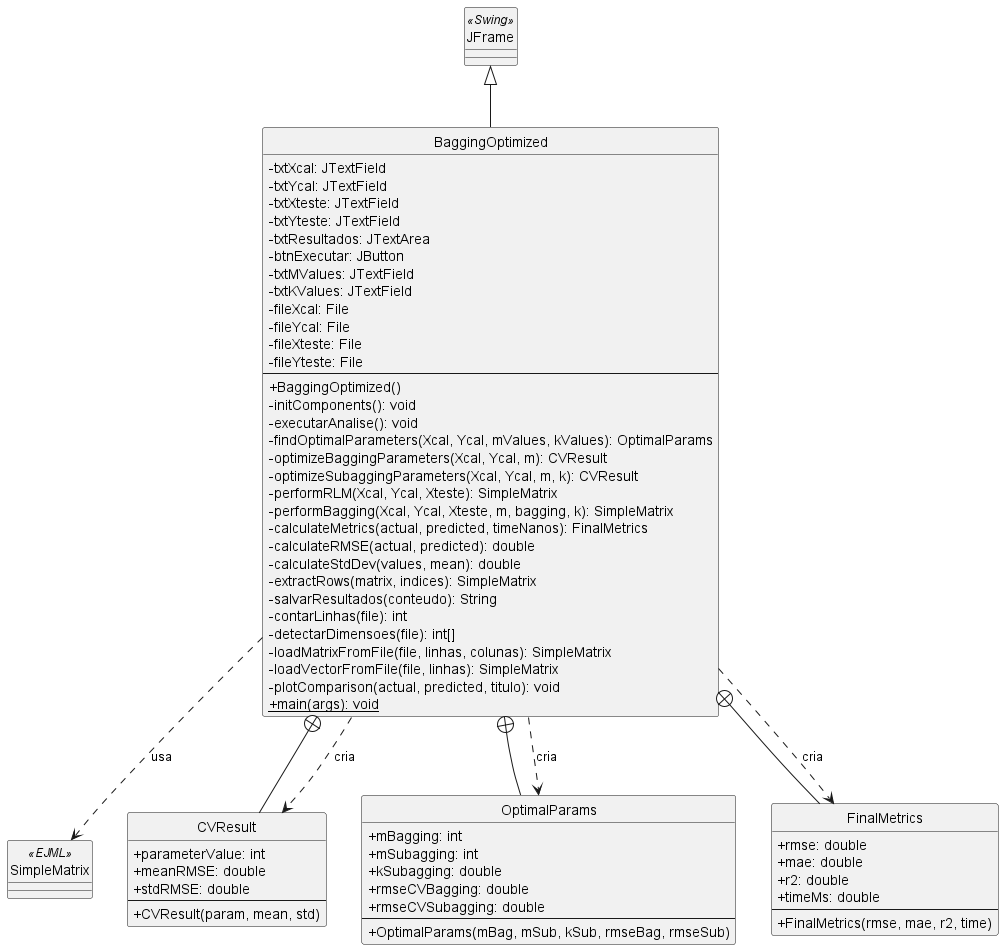
\includegraphics[width=1.00\textwidth]{./outros/fig/E_Diagramas/out/diag_classe/BaggingOptimized_Classe.png}
	\caption*{Fonte: \oautor}
	\label{fig:BaggingOptimized_Classe}
\end{figure}

\newpage
\section{Diagrama de Atividade --- Java}
\label{sec:diagatividadejava}

\begin{figure}[htbp]
	\caption{Diagrama de atividades.}
	\centering
		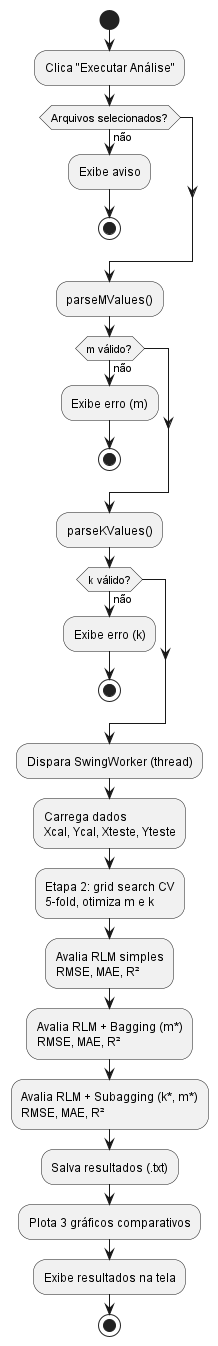
\includegraphics[width=0.20\textwidth]{./outros/fig/E_Diagramas/out/diag_sequencia/BaggingOptimized_Atividade.png}
	\caption*{Fonte: \oautor}
	\label{fig:BaggingOptimized_atividades}
\end{figure}

\newpage
\section{Diagrama de Sequência --- Java}
\label{sec:diagsequenciajava}

\begin{figure}[htbp]
	\caption{Diagrama de sequência.}
	\centering
		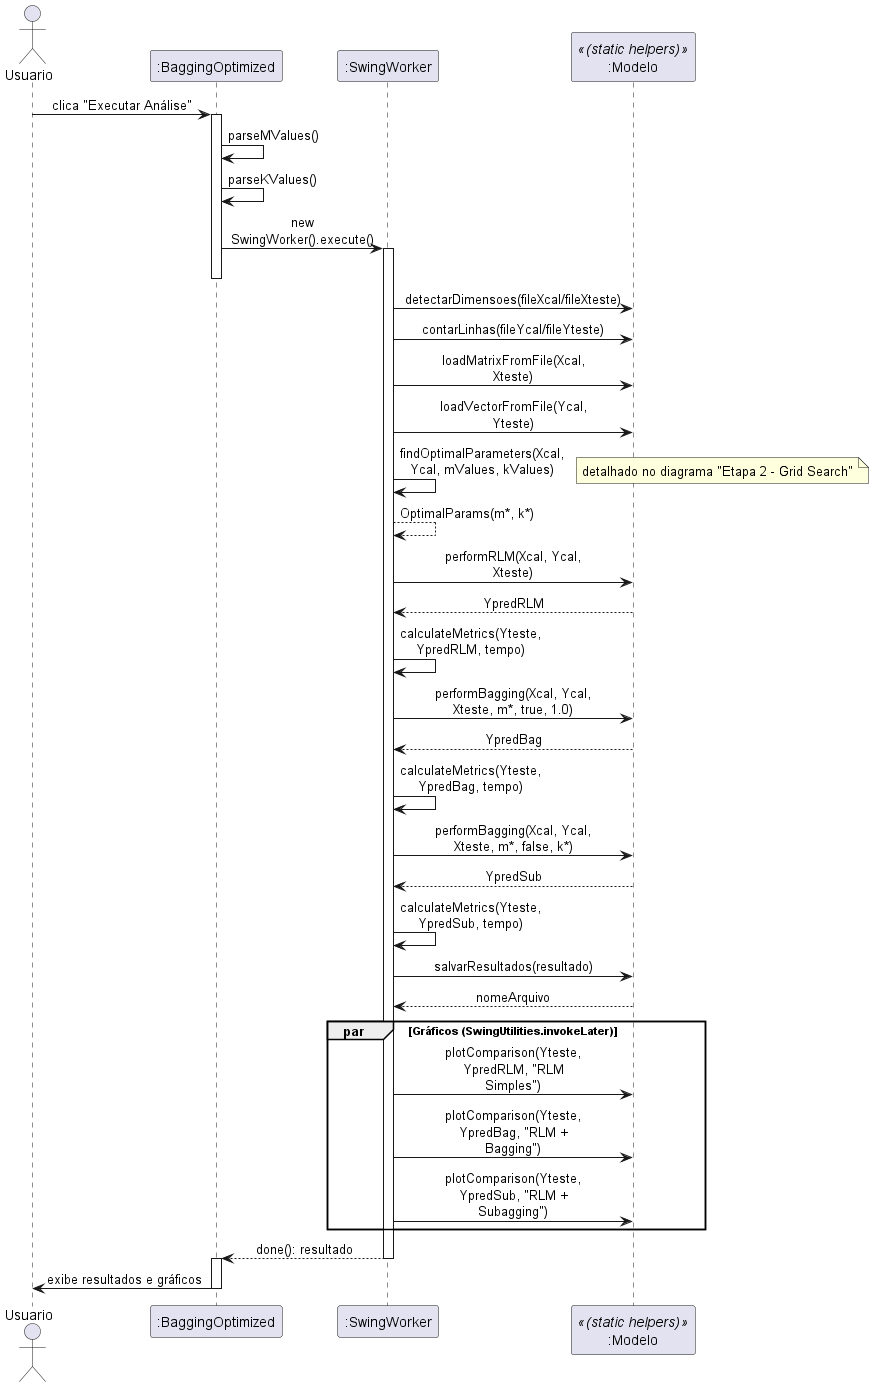
\includegraphics[width=0.75\textwidth]{./outros/fig/E_Diagramas/out/diagrama/BaggingOptimized_FluxoCompleto.png}
	\caption*{Fonte: \oautor}
	\label{fig:BaggingOptimized_sequencias}
\end{figure}

\newpage
\section{Diagrama de Atividades --- Java (PlantUML)}
\label{sec:diagatividadejavaplantuml}

\begin{figure}[htbp]
	\caption{Diagrama de atividade Java PlantUML .}
	\centering
		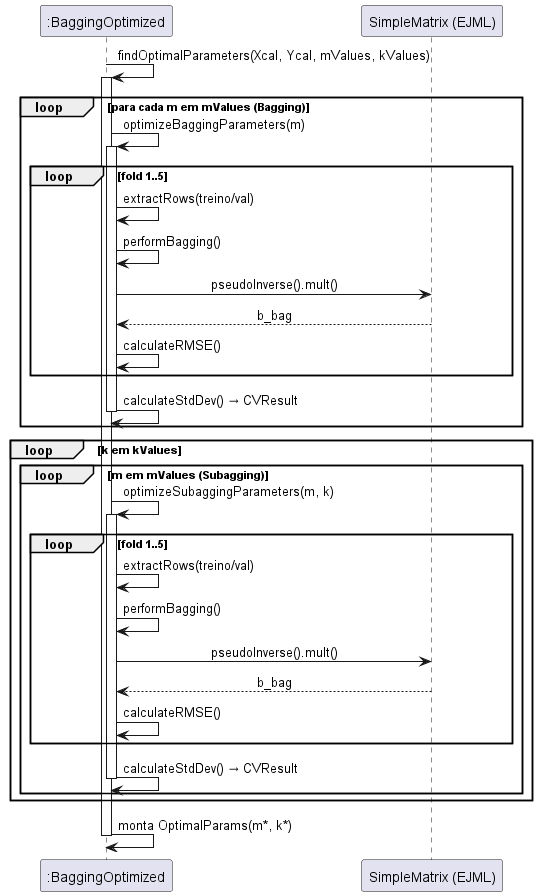
\includegraphics[width=0.50\textwidth]{./outros/fig/E_Diagramas/out/diagrama02/Etapa2_GridSearch_CV.png}
	\caption*{Fonte: \oautor}
	\label{fig:BaggingOptimized_atividade}
\end{figure}

\newpage
\section{Diagrama de Atividades --- Streamlit}
\label{sec:diagatividadestreamlit}

\begin{figure}[htbp]
	\caption{Diagrama de atividade Python PlantUML.}
	\centering
		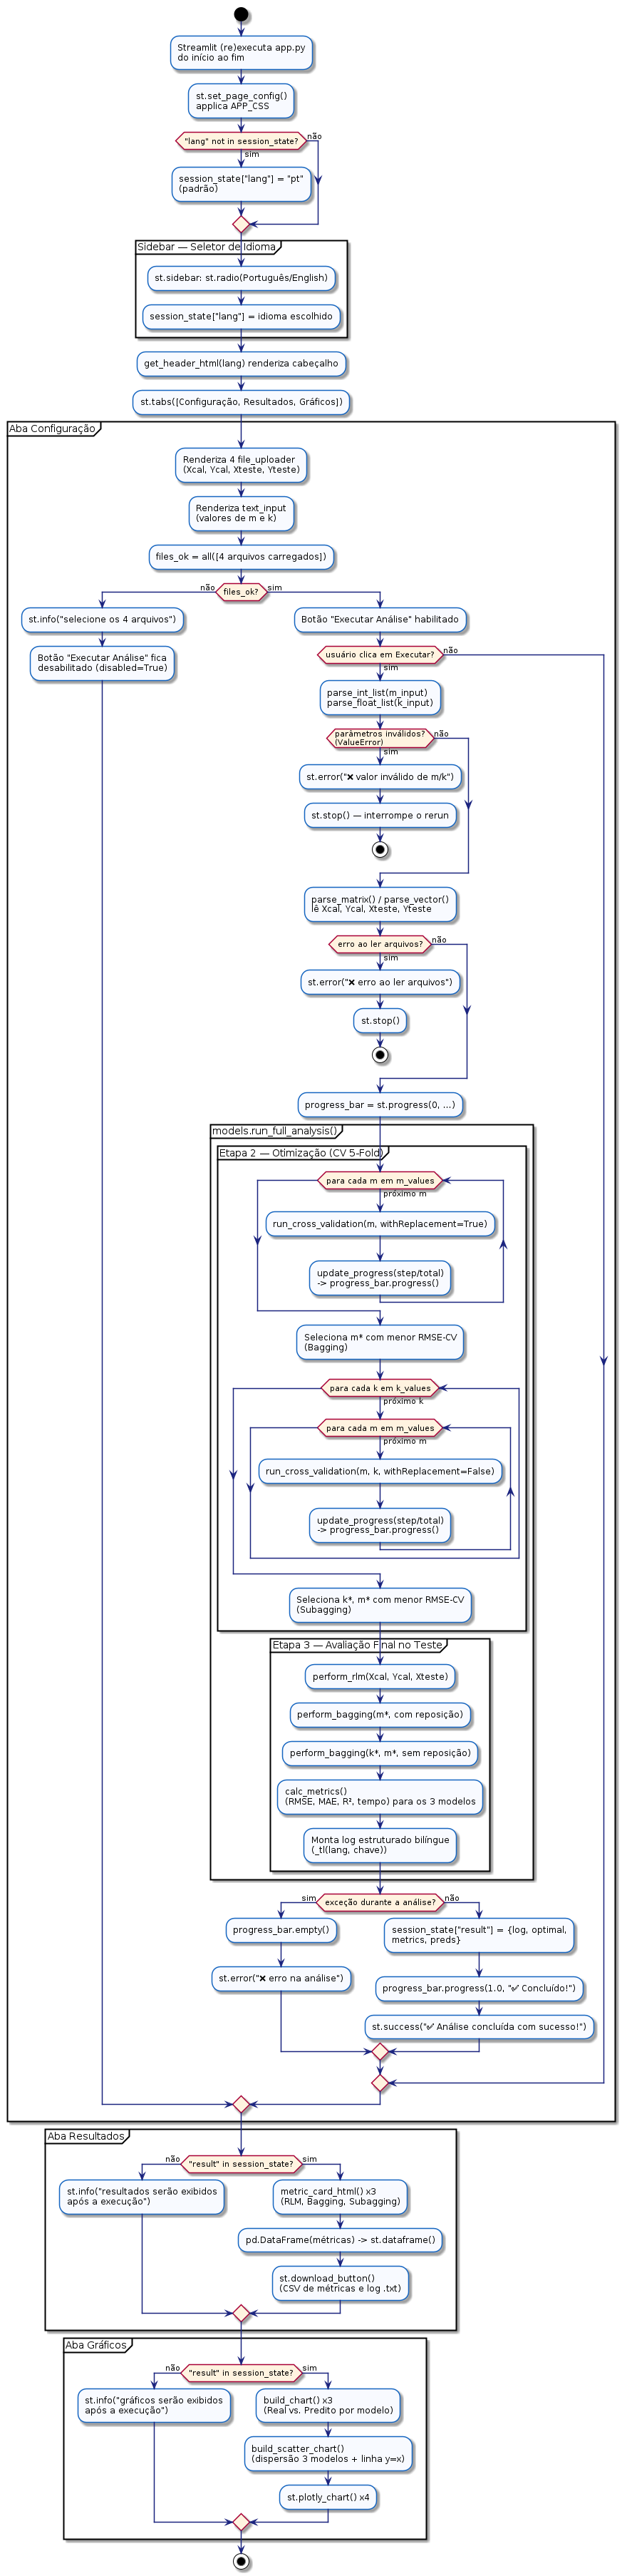
\includegraphics[width=0.30\textwidth]{./outros/fig/E_Diagramas/streamlit/diagrama_atividades_streamlit.png}
	\caption*{Fonte: \oautor}
	\label{fig:BaggingOptimized_atividade2}
\end{figure}

\newpage
\section{Diagrama de Classes (Módulos) --- Streamlit}
\label{sec:diagclassesstreamlit}

\begin{figure}[htbp]
	\caption{Diagrama de classes (módulos) PlantUML.}
	\centering
		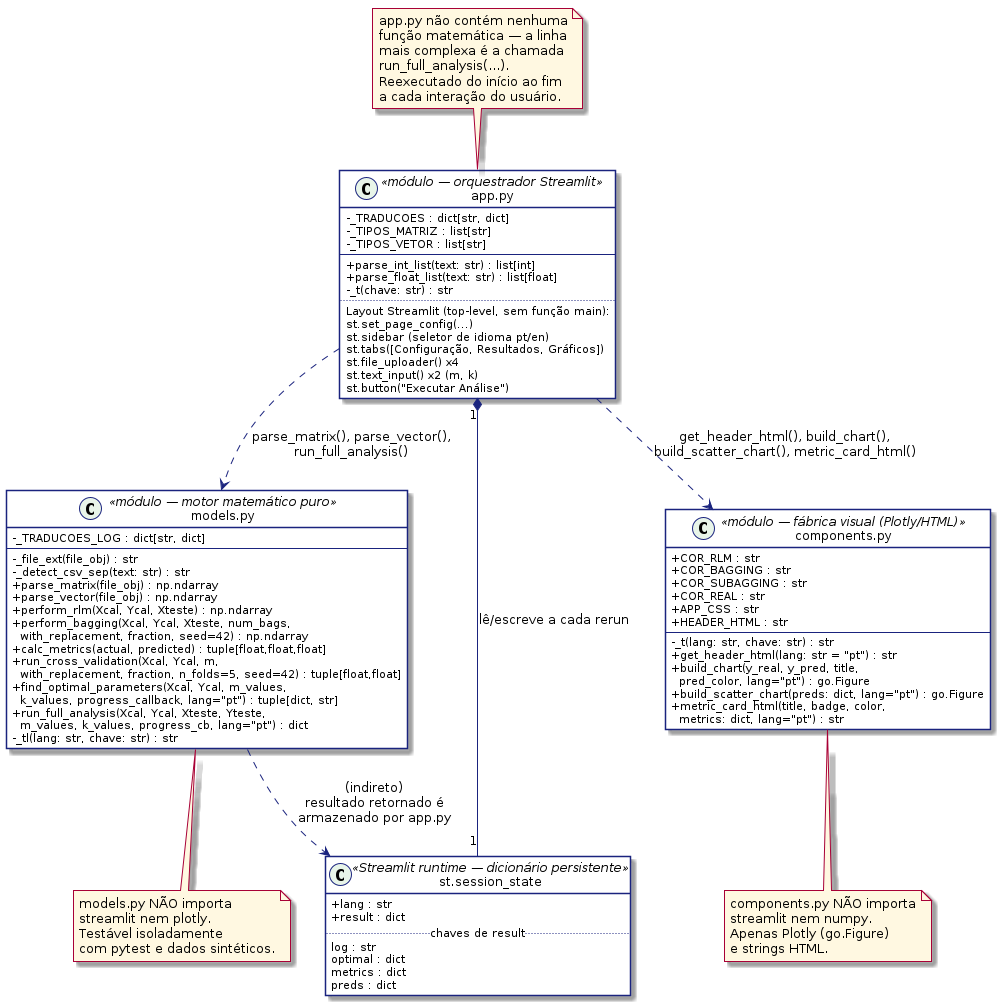
\includegraphics[width=0.85\textwidth]{./outros/fig/E_Diagramas/streamlit/diagrama_classes_streamlit.png}
	\caption*{Fonte: \oautor}
	\label{fig:BaggingOptimized_classe3}
\end{figure}

\newpage
\section{Diagrama de Sequência --- Streamlit}
\label{sec:diagsequenciastreamlit}

\begin{figure}[htbp]
	\caption{Diagrama de sequência PlantUML.}
	\centering
		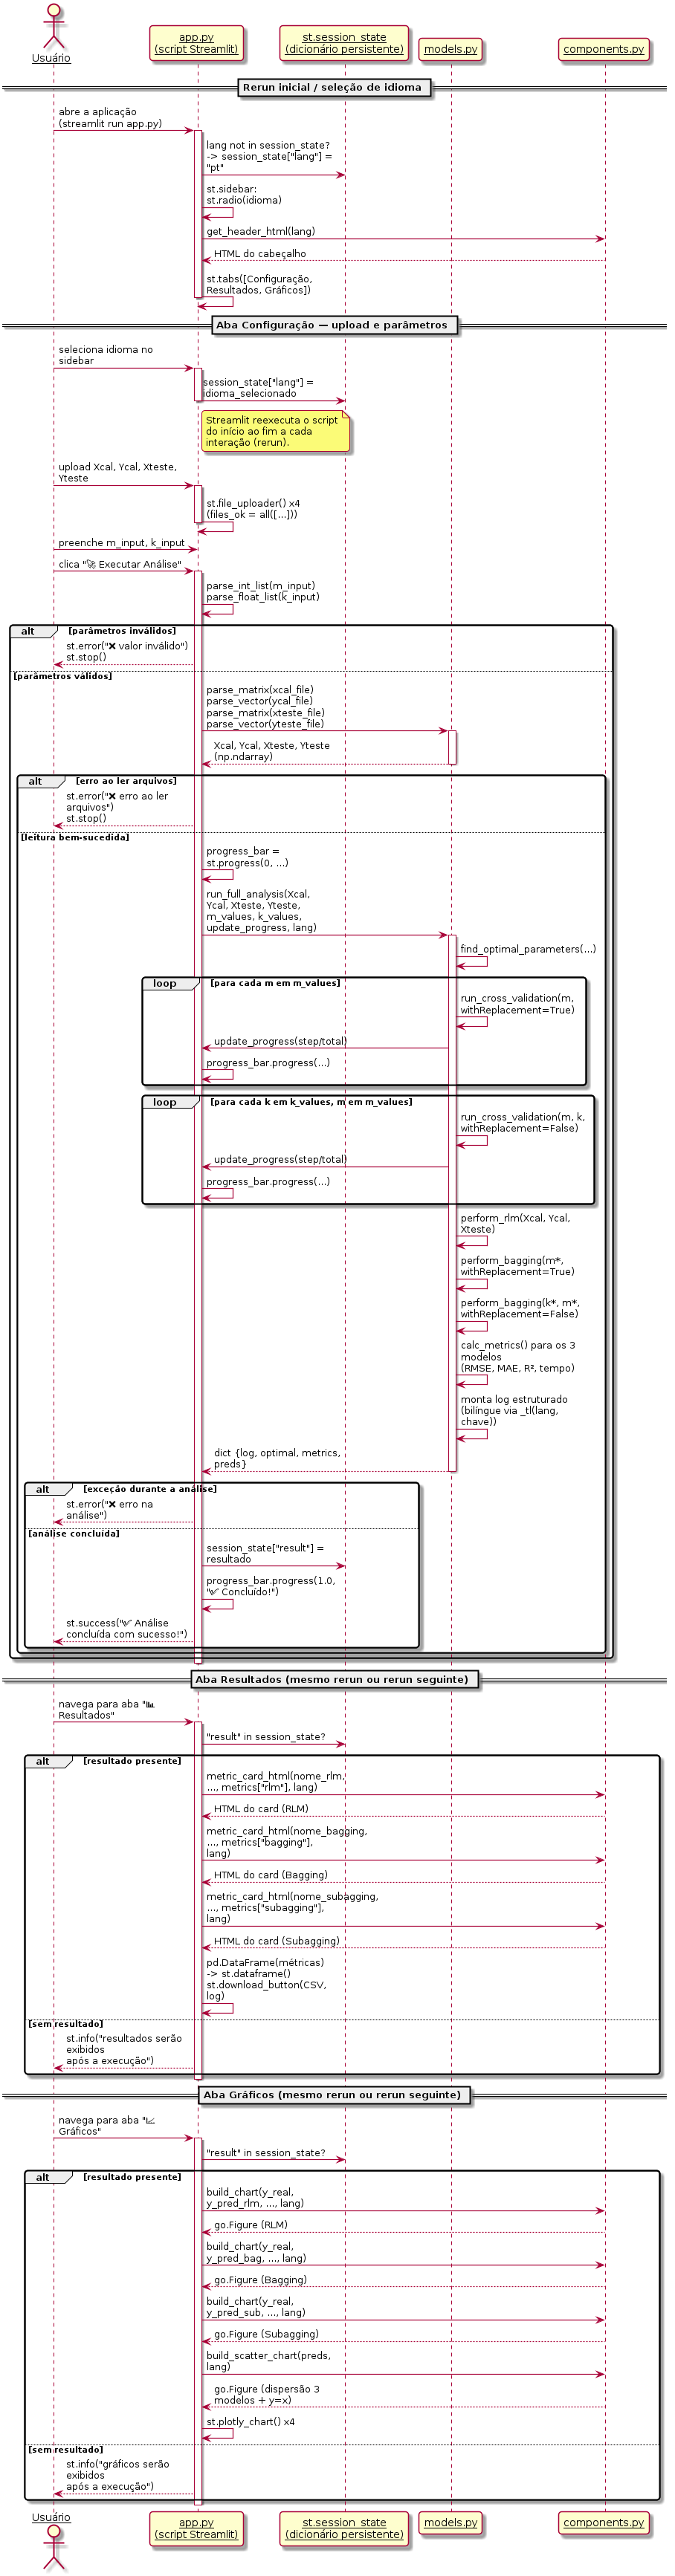
\includegraphics[width=0.30\textwidth]{./outros/fig/E_Diagramas/streamlit/diagrama_sequencia_streamlit.png}
	\caption*{Fonte: \oautor}
	\label{fig:BaggingOptimized_sequencia2}
\end{figure}

%Para retirar utilize a %
% ----------------------------------------------------------
\chapter{Diagrama}
\label{cha:diagrama}
\index{Diagrama}
% ----------------------------------------------------------
\begin{figure}[H]
    \centering
		    \caption{Diagrama de arquitetura em camadas (Java + Python)}
    \label{fig:meu_diagrama}
    \begin{tikzpicture}[
        layer/.style={draw, rounded corners, minimum width=8cm, 
                      minimum height=1.2cm, align=center, fill=#1},
        arrow/.style={-{Stealth}, thick}
    ]
        \node[layer=blue!15] (apresentacao) {Camada de Apresentação\\(Interface / API)};
        \node[layer=green!15, below=0.8cm of apresentacao] (negocio) {Camada de Lógica\\(Java + Python)};
        \node[layer=orange!15, below=0.8cm of negocio] (dados) {Camada de Dados\\(CSV / TXT)};
        
        \draw[arrow] (apresentacao) -- (negocio);
        \draw[arrow] (negocio) -- (dados);
    \end{tikzpicture}
	\caption*{Fonte: \oautor}
	\label{fig:diagramaarquitetura}
\end{figure}


%---------------------------------------------------
\begin{comment}
	
	\begin{figure}[H]
\centering
\begin{tikzpicture}[
    % Estilos das camadas
    layer/.style={
        draw, rounded corners=4pt, minimum width=11cm, 
        minimum height=1.4cm, align=center, font=\small\sffamily
    },
    component/.style={
        draw, rounded corners=2pt, minimum width=3.5cm, 
        minimum height=0.9cm, align=center, font=\scriptsize\sffamily
    },
    arrow/.style={-{Stealth[length=3mm]}, thick},
    label text/.style={font=\footnotesize\itshape}
]

% ===== CAMADA 1: APRESENTAÇÃO / ENTRADA =====
\node[layer, fill=blue!15] (entrada) at (0, 6) 
    {Camada de Entrada -- Dados dos Analitos (Cr, Fe, Mn, Ni, Mo)};

% ===== CAMADA 2: PROCESSAMENTO (Java + Python) =====
\node[layer, fill=green!15, minimum height=3.2cm] (processamento) at (0, 3) {};

% Subcamada Java
\node[component, fill=orange!20] (java) at (-3.5, 3.8) 
    {\textbf{Motor Java}\\(Weka / MOA)};
\node[component, fill=orange!10, font=\tiny\sffamily] (tecnicas_j) at (-3.5, 2.8) 
    {RLM $\cdot$ Bagging $\cdot$ Subagging};

% Subcamada Python
\node[component, fill=purple!20] (python) at (3.5, 3.8) 
    {\textbf{Motor Python}\\(scikit-learn)};
\node[component, fill=purple!10, font=\tiny\sffamily] (tecnicas_p) at (3.5, 2.8) 
    {RLM $\cdot$ Bagging $\cdot$ Subagging};

% ===== CAMADA 3: VALIDAÇÃO / PARIDADE =====
\node[layer, fill=yellow!20] (validacao) at (0, 0.5) 
    {Camada de Validação -- Paridade ($\Delta = |Y_{Python} - Y_{Java}| = 0$)};

% ===== SETAS DE FLUXO =====
\draw[arrow] (entrada.south) -- node[right, label text]{CSV} (processamento.north);
\draw[arrow] (processamento.south) -- node[right, label text]{Predições} (validacao.north);

% Conexões internas
\draw[-{Stealth[length=2mm]}, dashed, gray] (java.south) -- (tecnicas_j.north);
\draw[-{Stealth[length=2mm]}, dashed, gray] (python.south) -- (tecnicas_p.north);

\end{tikzpicture}
\caption{Diagrama de arquitetura em camadas do sistema de predição (Java + Python) para os analitos Cr, Fe, Mn, Ni e Mo.}
\label{fig:arquitetura_camadas}
\end{figure}

\end{comment}
%---------------------------------------------------

%Para retirar utilize a %


\end{apendicesenv}
% ---------------------------------------------------------

% ---------------------------------------------------------
% Inicia os anexos
% ---------------------------------------------------------
\begin{anexosenv}
%\partanexos*%Para desabilitar colocoque o %
%% ----------------------------------------------------------
\chapter{Descrição}
% ----------------------------------------------------------

São documentos não elaborados pelo autor que servem como fundamentação (mapas, leis, estatutos). Deve ser precedido da palavra ANEXO, identificada por letras maiúsculas consecutivas, travessão e pelo respectivo título. Utilizam-se letras maiúsculas dobradas quando esgotadas as letras do alfabeto. 
%Retirado
\end{anexosenv}

%---------------------------------------------------------------------
% INDICE REMISSIVO
%---------------------------------------------------------------------
%\phantompart
%\printindex
%---------------------------------------------------------------------

\end{document}
